%---------------------Settings---------------------------%
\documentclass[10pt,a4paper,twocolumn,twoside,UTF8]{article}
\usepackage{geometry}
	\geometry{left=1.8cm,right=1.8cm,top=2.5cm,bottom=2cm}
% \usepackage{xeCJK}
\usepackage{amsmath,paralist,enumitem,booktabs,multirow,graphicx,subfig,setspace,listings,multicol,lettrine}
	\setlength{\parindent}{2em}
	\lstset{language=Python}
\usepackage{fancyhdr}
\usepackage{layout}
\setlength\columnsep{0.8cm}

%%begin----------Set header and footer----------------%%
\usepackage{ifthen}
\newboolean{first}
\setboolean{first}{true}
\pagestyle{fancy}
	\fancypagestyle{maincontent}{
		\fancyhf{}  
		\fancyhead[EL, OR]{\thepage}
		\fancyhead[EC]{C7 SLM-based optical experiment}
		\fancyhead[OC]{GENERAL PHYSICS LABORATORY}
		\renewcommand\headrulewidth{0pt}
	}
	
	\usepackage{datetime}
	\fancypagestyle{firstpage}{
		\setboolean{first}{false}
		\fancyhf{}  
		\fancyhead[L]{Sun Yat-sen University}
		\fancyhead[R]{\shortmonthname[\the\month], \the\year}
		\fancyhead[C]{
		          \large{GENERAL PHYSICS LABORATORY}
		          }
	}
	
	\newcommand{\makefirstpageheadrule}{
	\makebox[0pt][s]{\rule[0.6\baselineskip]{\headwidth}{0.3pt}}
	\makebox[0pt][s]{\protect\hspace{-0.34em}\rule[0.75\baselineskip]{\headwidth}{0.3pt}}
	\protect\vspace{-20pt}
	}

	\newcommand{\makeheadrule}{
	\makebox[0pt][l]{\rule[1\baselineskip]{\headwidth}{0.3pt}}
	\protect\vspace{-20pt}
	}

	\renewcommand{\headrule}{
	\ifthenelse{\boolean{first}}{\makeheadrule}
	{\makefirstpageheadrule}
	}
%%end--------------Set header and footer-----------%%

%%begin-----------------Reference-----------------------%%
\usepackage[colorlinks,linkcolor=blue,urlcolor=blue,citecolor=blue]{hyperref}
\usepackage[hyperref=true,backend=biber,bibstyle=science,citestyle=numeric-comp,sorting=none,backref=true]{biblatex}
\addbibresource{REF.bib}
%%end-------------------Reference-----------------------%%

%end---------------------Settings---------------------------%




%%%%%%%%%%%%%%%%%%%%%%%%%%%%%%%%%%%%%%%%%%%%%%%%%%%%%%%%%%
%%%%%%%%%%%%%%%%%%%%%%%%%Document%%%%%%%%%%%%%%%%%%%%%%%%%
%%%%%%%%%%%%%%%%%%%%%%%%%%%%%%%%%%%%%%%%%%%%%%%%%%%%%%%%%%

%%begin-------------------Abstract-----------------------%%
\begin{document}
\title{\LARGE\textbf{SLM-based optical experiment} \footnotemark[1]}
\author{\large\textit{Zweig, Wong}$^{1}$\footnotemark[2]
\\ \normalsize{1 Zhongshan School of Medicine, Sun Yat-sen University, Guangzhou  { \rm 510275}, China}}
\date{}

\twocolumn[
	\begin{@twocolumnfalse}
	\maketitle  
	\renewcommand{\abstractname} {} 
	\begin{abstract}
	\vspace{-3em}
	{\bf Abstract: }
	{\small 
    Spatial Light Modulation (SLM) is an optical element capable of modulating the physical quantities of the optical field as required by the input control signal.
	With the advantages of portability and versatility of SLM, it has been widely used in optical experiments and engineering.
	In this research, we conducted a series of classical optical experiments based on SLM to study different optical phenomena as well as to investigate and verify the effectiveness of SLM as a replacement for traditional optical elements.
	First, we investigated the amplitude modulation performance of the SLM and found that there existed a threshold before which SLM didn't respond to the change of gray scale.
	Next, using an SLM loaded with the checker image as an object, we measured the distortion of images in different convex lens imaging system. 
	Then, using SLM loaded with an optical grating image as object, we conducted optical information processing experiments, including verifying Abbe's theory of image formation and spatial filtering experiments.
	Finally, as one of the most important fields of SLM's applications, holographic techniques including computational holography and digital holography based on SLM were applied to generate and restore the holograms.
	All experiments proved the high performance and effectiveness of SLM as a replacement of traditional optical elements.
	In conclusion, in this research we have revealed the performance of SLM as an optical element in different optical experiments and thus provided a deeper insight into the application of SLM.

	}
	\par
	\textbf{Keywords: Spatial Light Modulation (SLM), Distortion, Optical information processing, Holography}
	\vspace{2em}
	\end{abstract}
	\end{@twocolumnfalse}
]

\renewcommand{\thefootnote}{\fnsymbol{footnote}}
\footnotetext[1]{Supported and taught by Luyoutang, School of Physics, Sun Yat-sen University}
\footnotetext[2]{Corresponding author. ID: 20980066 Email: \url{huangzw29@mail2.sysu.edu.cn} }
%%end-------------------Abstract-----------------------%%

\thispagestyle{firstpage} 
\pagestyle{maincontent}

%%begin-------------------Intro-----------------------%%
\section{Introduction}
\lettrine[lines=2]{S}{patial} Light Modulation (SLM) is an optical element capable of modulating the physical quantities of the optical field such as amplitude, phrase and polarization as required by the input control signal.
The most commonly used SLM is twisted nematic liquid-crystal spatial light modulator (TNLC-SLM), whose working medium is liquid crystals disposing in specific twisting arrangement. In response to different control voltages, 
directors of liquid crystal molecules will rotate to specific directions, resulting in changes of optical properties and thus modulation of the input light.
With different images loaded, SLM is capable of serving as a virtual object or optical grating. On the basis of this property, TNLC-SLM has been widely used in optical experiments. 

In this research, based on SLM, we conducted three experiments: measuring the distortion of the convex lens imaging system, optical information processing, as well as generating and restoring the holograms.
Distortion of convex lens imaging system is a non-paraxial effect in which parts of object far away from the axis have different and nonuniform amplification ratio, resulting in lost of similarity.
Optical information processing is a new effective information processing technique that uses light as an information carrier and actually performs the processing directly based on optical modulation of the properties of light. 
Compared to digital information processing, it supports parallel processing of a large volume of data in high resolution in a short time and does not require sampling-restoration procedure, thus being suitable for image processing.
Holography is a new-generation photographic techniques which records all information of the light field including amplitude and phrase basing on interference principles. 
With rapid development in this field, new holographic techniques including computational holography and digital holography has emerged and got widely applied in 3D display, virtual reality and so on.
By conducting these optical experiments based on SLM, we aimed to investigate different optical phenomena in these systems and to verify the effectiveness of SLM as an optical element.

%%end-------------------Intro-----------------------%%
% \newpage % Change the column
%%begin-----------------Method-----------------------%%
\section{Experimental principles and method}
	\subsection{Experimental principle\autocite{shenGeneralPhysicsLaboratory2015}}
		\subsubsection{Transmissive Twisted nematic liquid-crystal spatial light modulator (TTNLC-SLM)\autocite{nguyenSpatialLightInterference2013}}
		The microstructure of transmissive twisted nematic liquid-crystal spatial light modulator is illustrated in Fig. \ref{fig.illus-1.1} and Fig. \ref{fig.illus-1.2}. 
		The central core part of the element is a two-dimensional microarray composing of lots of small twisted nematic liquid-crystal box (TNLC box). 
		Each box, known as a pixel, is a stand-alone unit that is capable of receiving and responding to the control voltage signal independently. 

		\begin{figure*}[htbp]
			\centering		
			\subfloat[Transmissive spatial light modulator]{\label{fig.illus-1.1}
			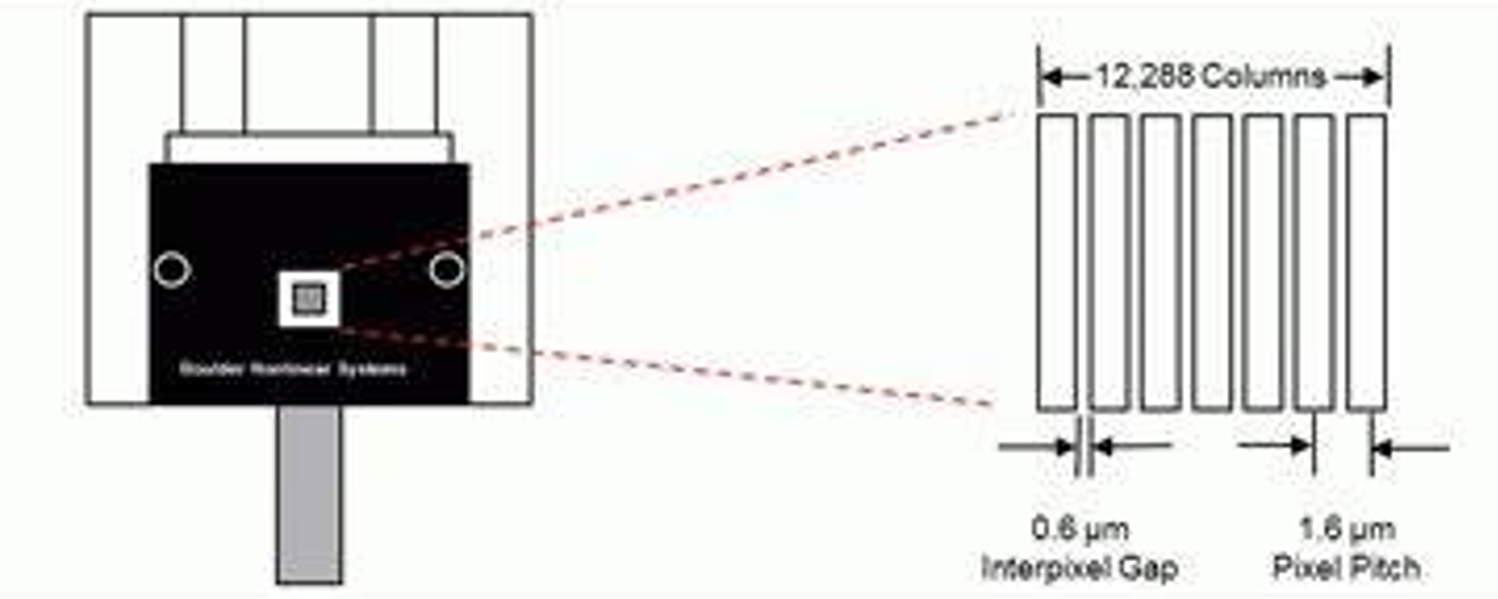
\includegraphics[width=0.4\textwidth]{attachments/fig.illus-1.1.png}
			}
			\subfloat[A TNLC box]{\label{fig.illus-1.2}
			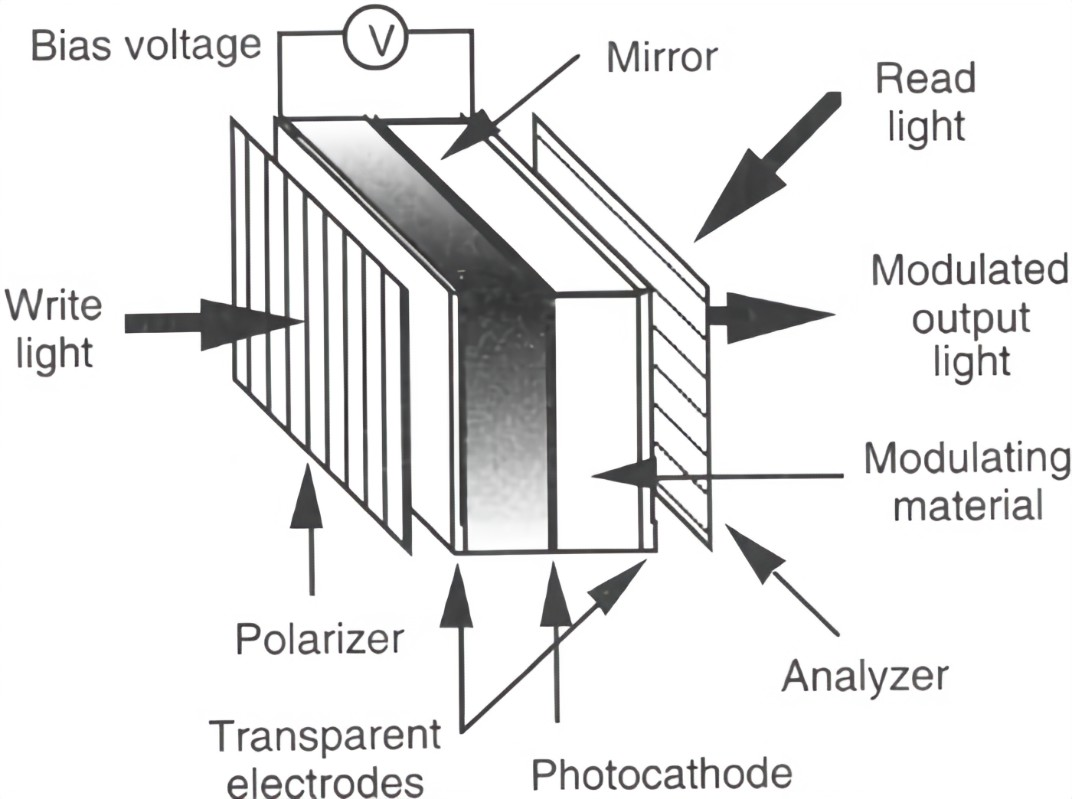
\includegraphics[width=0.4\textwidth]{attachments/fig.illus-1.2.png}
			}
			\caption{\textbf{Transmissive Twisted nematic liquid-crystal spatial light modulator (TTNLC-SLM)}}
		\end{figure*}

		As illustrated in Fig. \ref{fig.illus-1.3} and Fig. \ref{fig.illus-1.4}, when there is no voltage between the electrodes, as an effect of the microstructure of the inner surface of the glasses, the liquid crystal molecules will arrange in a "twisted" manner, that is, the directors of molecules will gradually rotate $90^o$ between the two surface. 
		Thus, the TNLC box without voltage loaded will behave as a linearly twisted anisotropic media, in which the polarization direction of the polarized light will rotate along with the directors of the molecules, thus there is a $90^o$ polarization angle difference between the input light and output light. 
		If an analyzer, whose direction is perpendicular to the polarization direction of the input light, is applied on the output surface, then, in this case without voltage, as the output light's polarization direction matches the direction of the analyzer, the box allows the passage of light.
		
		However, when a control voltage signal is applied between the electrodes, because the liquid crystal molecules are polar molecules, they tend to arrange along the electric field, and thus the "twisted" arrangement is broken. 
		In this case, the polarization direction of input light will not or just slightly change when passing through the liquid crystal box, and thus will be partly or completely blocked by the analyzer. 
		
		\begin{figure*}[htbp]
			\centering		
			\subfloat[Polarization effect of the TNLC box]{\label{fig.illus-1.3}
			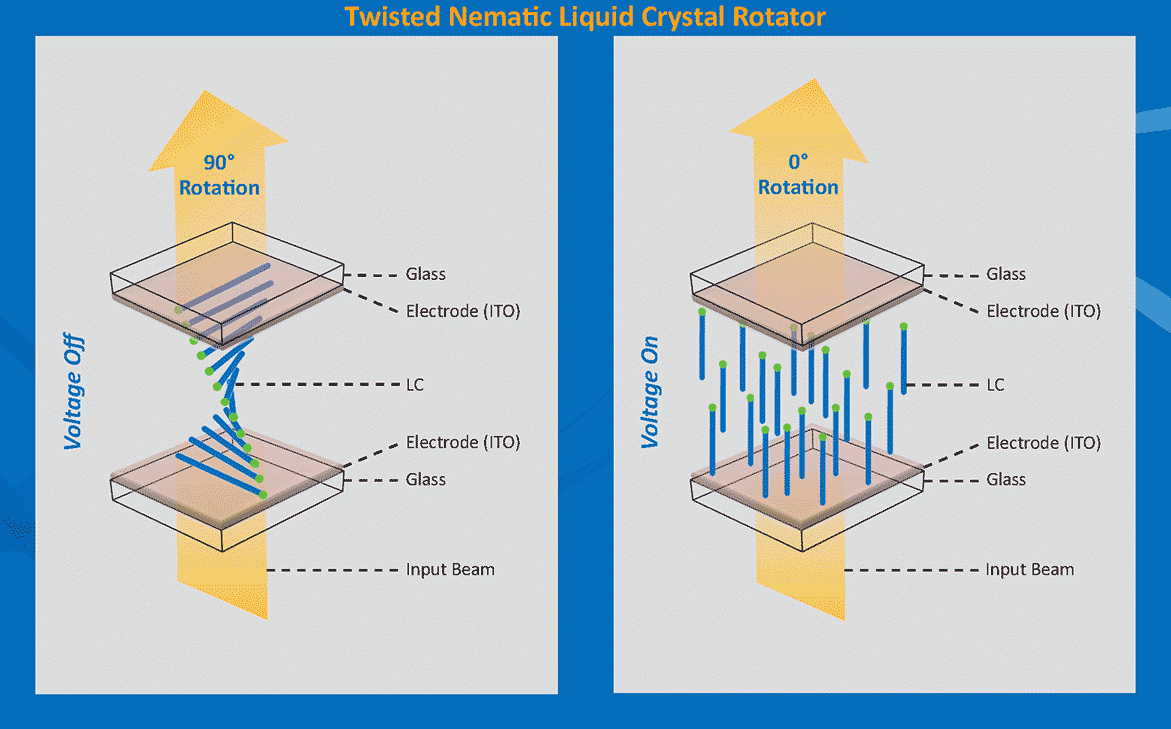
\includegraphics[width=0.4\textwidth]{attachments/fig.illus-1.3.png}
			}
			\subfloat[TNLC box respond to the control voltage]{\label{fig.illus-1.4}
			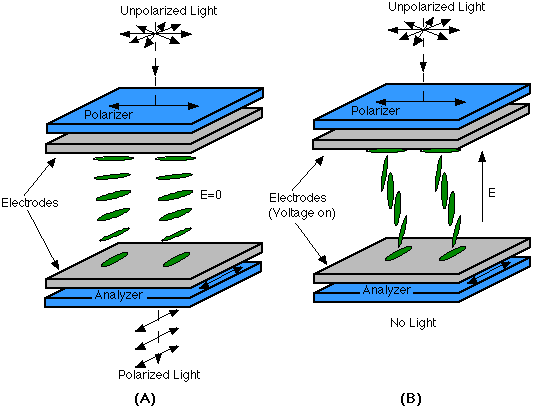
\includegraphics[width=0.4\textwidth]{attachments/fig.illus-1.4.png}
			}
			\caption{\textbf{Mechanism of TTNLC-SLM}}
		\end{figure*}

		The transmissivity of the TNLC box ($T$) in response to control voltage can be calculated by Eq. \ref{eq.1.1}
		\begin{align}
			T = &[\frac{\pi}{2\gamma}sin(\gamma)cos(\phi_1-\phi_2)+cos(\gamma)sin(\phi_1-\phi_2)]^2 + \notag\\
				&[\frac{\beta}{\gamma}sin(\gamma)sin(\phi_2+\phi_1)]^2 
			\label{eq.1.1}
		\end{align}
		
		where $\gamma = \sqrt{\psi_d^2 + (\frac{\pi(n_e-n_0)d}{\lambda})^2}$, $\psi_d$ is the total rotation angle, $d$ is the thickness of the box, $\lambda$ is the wavelength, $n_e$ is the refractive index in response of different voltage:

		\begin{equation}
			\frac{1}{n_e^2(\theta)} = \frac{cos^2(\theta)}{n_e^2} + \frac{sin^2(\theta)}{n_0^2}
			\label{eq.1.2}
		\end{equation}
		
		where $\theta$ satisfies:

		\begin{align}
			\theta =
			&\left\{
				\begin{aligned}
					&0 &,V_s \le V_c \\
					&\frac{\pi}{2} - 2tan^{-1}[e^{-\frac{V_s - V_c}{V_0}}] &,V_s > V_c \\
				\end{aligned}
			\right. \\
			\label{eq.1.3}
		\end{align}
		$V_s$ is the loaded voltage, $V_c$ is the threshold voltage, $V_0$ is the voltage where $\theta = 49.6^o$.
		
		Obviously, if $V_s < V_c$, there is no modulation effect as the voltage is not sufficient to twist the molecules; as the voltage increases, the twisting effect of the electric field increases, thus the transmissivity decreases predominantly.
		
		
		\subsubsection{Distortion of convex lens imaging system}
		Distortion of convex lens imaging system is a non-paraxial effect in which parts of an object far away from the axis have different and non-uniform amplification ratios, resulting in a loss of similarity. 
		There are two types of distortion, named "barrel distortion" and "pincushion distortion", as illustrated in Fig. \ref{fig.illus-2.1}.

		The relative distortion can be calculated by Eq. \ref{eq.2.1}
		\begin{equation}
			q = \frac{Y'_2 - Y_2}{Y_2} \times 100\%
			\label{eq.2.1}
		\end{equation}
		where $q$ is the relative distortion, $Y'_2$ is the actual image height,  $Y_2$ is the ideal image height, $Y_2 = VY_1$.
		The optical path is illustrated in Fig. \ref{fig.illus-2.2}
		\begin{figure*}[htbp]
			\centering		
			\subfloat["barrel distortion" and "pincushion distortion"]{\label{fig.illus-2.1}
			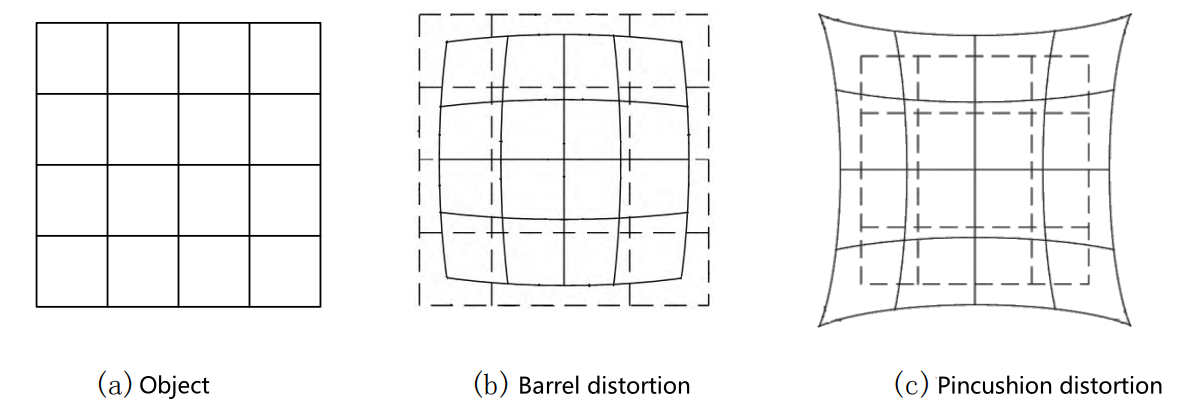
\includegraphics[width=0.4\textwidth]{attachments/fig.illus-2.1.png}
			}
			\subfloat[Light path]{\label{fig.illus-2.2}
			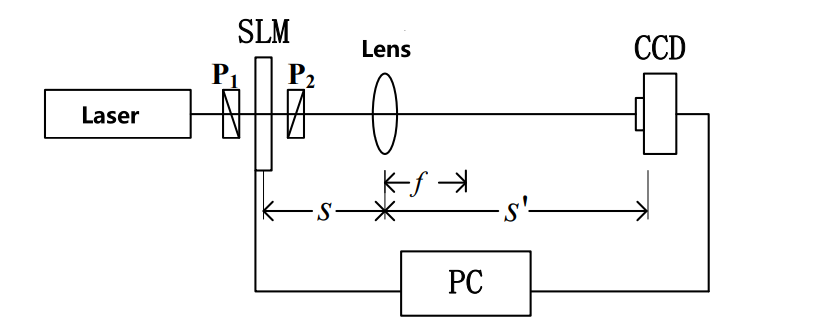
\includegraphics[width=0.4\textwidth]{attachments/fig.illus-2.2.png}
			}
			\caption{\textbf{Distortion of convex lens imaging system}}
		\end{figure*}

		\subsubsection{Optical information processing and spatial filtering}
		\paragraph{A. Abbe's theory of image formation and principles of spatial filtering}~
		\newline 
		\indent
		Abbe's theory considers image formation in two stages. 
		The first stage is formation of a spatial spectrum in a rear focal plane of a lens ($P_2$, known as the Fourier plane ). 
		The second stage is formation of a image in the image plane ($P_3$) as a result of interference of beams coming from $P_2$. (Fig. \ref{fig.illus-3.1})
		\begin{figure}[htbp]
			\centering
			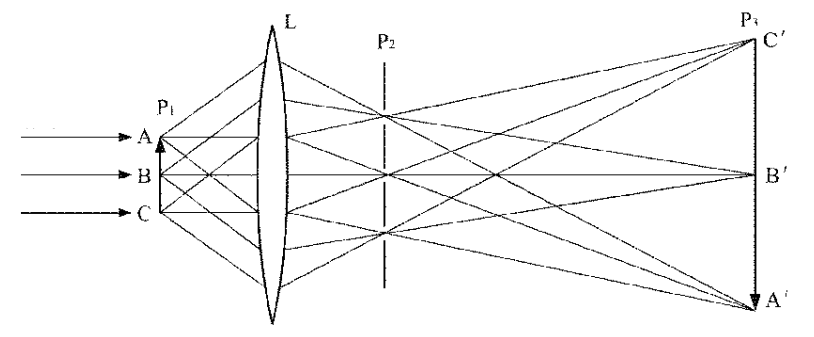
\includegraphics[width=0.4\textwidth]{attachments/fig.illus-3.1.png}
			\caption{\textbf{Abbe's theory of image formation}}
			\label{fig.illus-3.1}
		\end{figure}

		By placing different spatial filters such as high-pass (Fig. \ref{fig.illus-3.2.1}), low-pass (Fig. \ref{fig.illus-3.2.2}) and band-pass filters (Fig. \ref{fig.illus-3.2.3}) 
		on the Fourier's plane $P2$ to modulate the spatial spectrum, this system can realize various of optical information processing effects.

		\begin{figure*}[htbp]
			\centering		
			\subfloat[High-pass filter]{\label{fig.illus-3.2.1}
			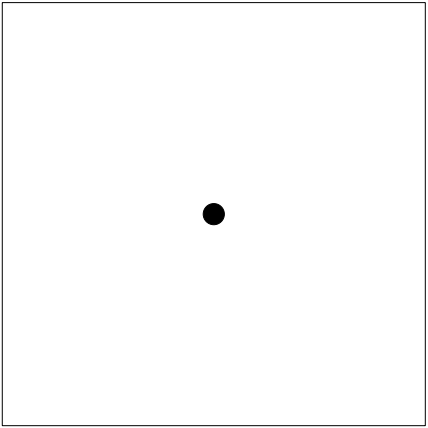
\includegraphics[width=0.3\textwidth]{attachments/fig.illus-3.2.1.png}
			}
			\subfloat[Low-pass filter]{\label{fig.illus-3.2.2}
			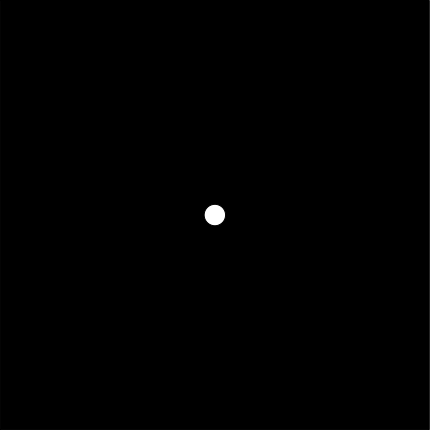
\includegraphics[width=0.3\textwidth]{attachments/fig.illus-3.2.2.png}
			}
			\subfloat[band-pass filter]{\label{fig.illus-3.2.3}
			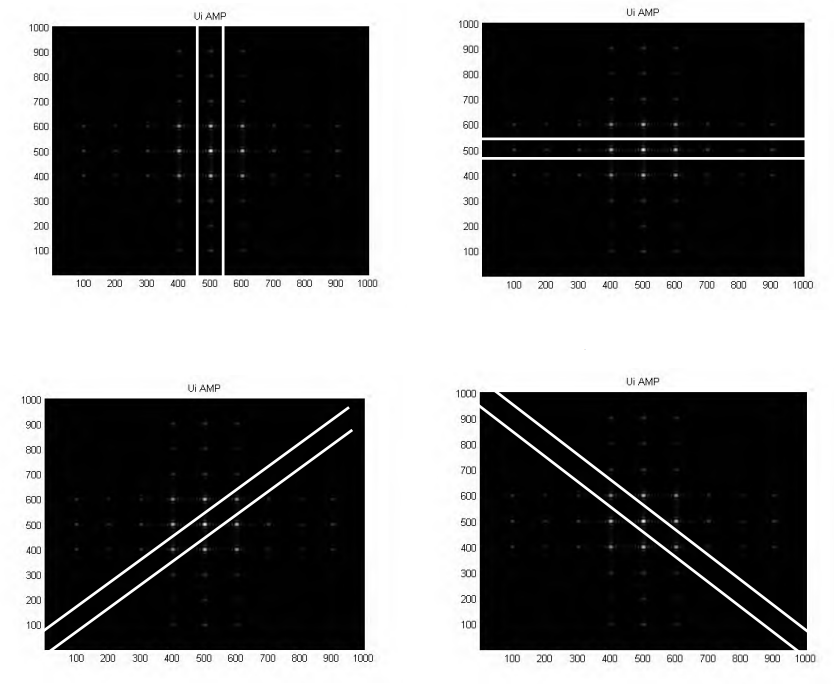
\includegraphics[width=0.3\textwidth]{attachments/fig.illus-3.2.3.png}
			}
			\caption{\textbf{Spatial filters}}
		\end{figure*}



		\paragraph{B. Optical information processing light path}~
		\newline 
		\indent
		There are two classical light paths for optical information processing. 
		The first one, known as "4f system", contains three lenses (Fig. \ref{fig.illus-4.1}). 
		A transparent object (which can be transmissive SLM with image loaded) is placed on the $P_1$ plane, and light passed through the object is focused by the lens $L_1$ on its back focus, which is on the $P_2$ plane (Fourier's plane). 
		The filter is placed on the $P_2$ plane to modulate the spatial spectrum. 
		According to Abbe's theory of image formation, interference of modulated beams coming from $P_2$ will generate the image in the image plane ($P_3$), which is the output information.

		Another light path is much simpler and contains only one lens (Fig. \ref{fig.illus-4.2}). 
		Parallel light passed through the object will be focused by the lens. 
		By placing the filter on the Fourier's plane to modulate the spatial spectrum, it can also realize optical information processing.

		\begin{figure*}[htbp]
			\centering		
			\subfloat[4f system]{\label{fig.illus-4.1}
			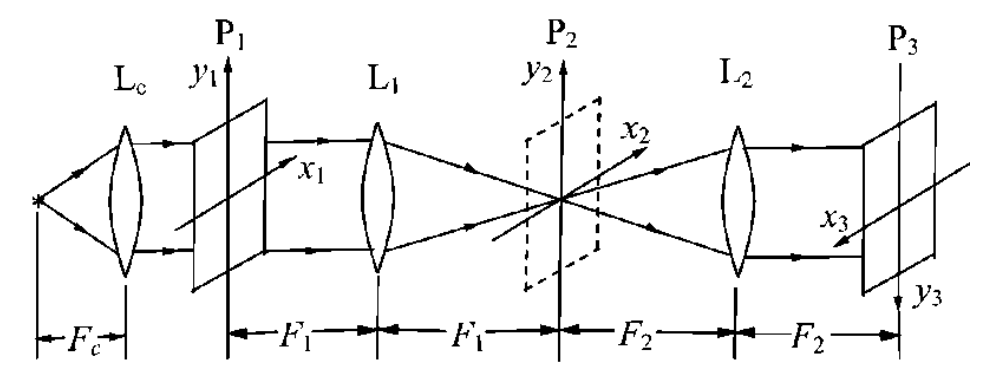
\includegraphics[width=0.4\textwidth]{attachments/fig.illus-4.1.png}
			}
			\subfloat[Single-lens system]{\label{fig.illus-4.2}
			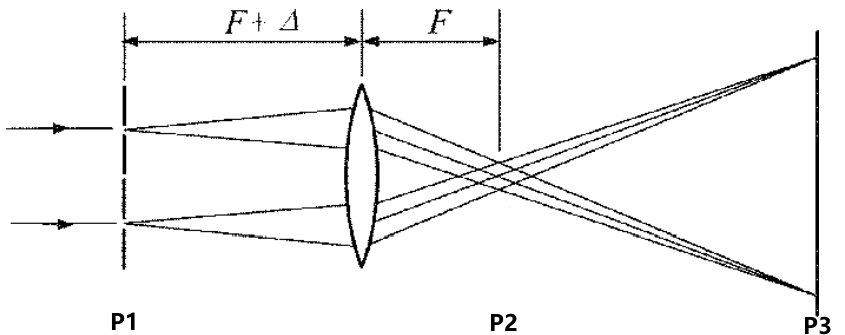
\includegraphics[width=0.4\textwidth]{attachments/fig.illus-4.2.png}
			}
			\caption{\textbf{Optical information processing light path}}
		\end{figure*}


		\subsubsection{Holography}
		Holography is a new-generation photographic technique which records all information of the light field including amplitude and phrase basing on interference principles.
		The principles of holography can be understood by studying traditional optical holography. 
		
		Holography generally contains two steps: wave front recording (Fig. \ref{fig.illus-5.1}) and wave front reconstruction (Fig. \ref{fig.illus-5.2}).
		In wave front recording, a reference light $R(x,y) = |R(x,y)|e^{i\psi(x,y)}$ is applied to interfere with the object light $O(x,y) = |O(x,y)|e^{i\phi(x,y)}$. 
		The interference light field $I(x, y)$ is recorded and used to prepare the holographic image. 
		\begin{align}
			I(x,y) =& |R(x,y)+O(x,y)|^2 \notag \\
				   =& |R(x,y)|^2+|O(x,y)|^2 + \notag \\
				    &2|R(x,y)||O(x,y)|cos(\phi-\psi) 
			\label{eq.5.1}
		\end{align}

		After processing, the transmissivity of the holographic image $t_A(x, y)$ is:
		\begin{equation}
			t_A(x, y) = t_b + \beta '(|O|^2 + R^*O + RO^*)
			\label{eq.5.2}
		\end{equation}

		In wave front reconstruction, a beam is applied, which is the same as the reference light used in wave front recording, to generate the reconstructed light field $Rt_A(x,y)$.
		\begin{equation}
			Rt_A(x, y) = t_bR + \beta '(|O|^2R + |R|^2O + RRO^*)
			\label{eq.5.3}
		\end{equation}

		\begin{figure*}[htbp]
			\centering		
			\subfloat[Wave front recording]{\label{fig.illus-5.1}
			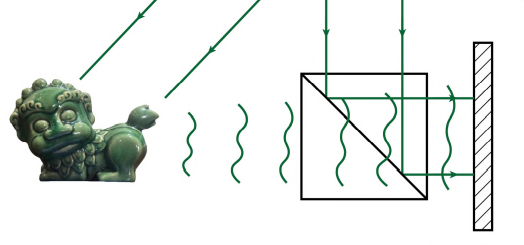
\includegraphics[width=0.4\textwidth]{attachments/fig.illus-5.1.png}
			}
			\subfloat[Wave front reconstructing]{\label{fig.illus-5.2}
			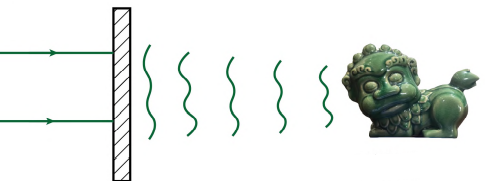
\includegraphics[width=0.4\textwidth]{attachments/fig.illus-5.2.png}
			}
			\caption{\textbf{Holography}}
		\end{figure*}

		With rapid development in this field, new holographic techniques including computational holography and digital holography have been developed to improve traditional optical holography, which requires very complex recording and processing procedures. 
		Different from the traditional optical holography, in which recording and reconstructing are both realized by optical systems, computational holography adopts a strategy called "Digital recording and optical reconstructing", 
		which means the holographic image is computed by holographic algorithm directly from the original image, and the reconstructing process is realized by optical system, which is the same as in optical holography. 
		As for digital holography, the holographic image is recorded in the optical system, which is the same as in optical holography, while the reconstructed image is computed from the holographic image by algorithm ("Optical recording and digital reconstructing"). 
		These new holographic techniques have been widely used in various fields such as 3D display and Virtual Reality.

		For computational holography, the light path is illustrated in Fig. \ref{fig.illus-5.3}. 
		The holographic image is loaded on the SLM, reference light is applied to beam the SLM, and the reconstructed image is recorded by the CCD. 

		Light path of digital holography is illustrated in Fig. \ref{fig.illus-5.4}. Laser is split into two beams by the prism. 
		One beam is used to beam the object to generate the object light field $O(x,y) = |O(x,y)|e^{i\phi(x,y)}$, and the other beam is used as the reference light $R(x,y) = |R(x,y)|e^{i\phi(x,y)}$. 
		The interference light field $I(x, y)$ is recorded by CCD, and the reconstructed image is calculated by the algorithm.

		\begin{figure*}[htbp]
			\centering		
			\subfloat[Computational holography]{\label{fig.illus-5.3}
			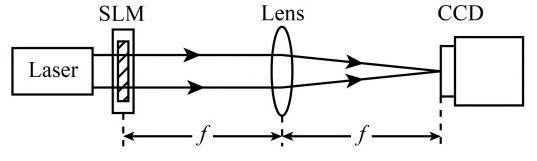
\includegraphics[width=0.4\textwidth]{attachments/fig.illus-5.3.png}
			}
			\subfloat[Digital holography]{\label{fig.illus-5.4}
			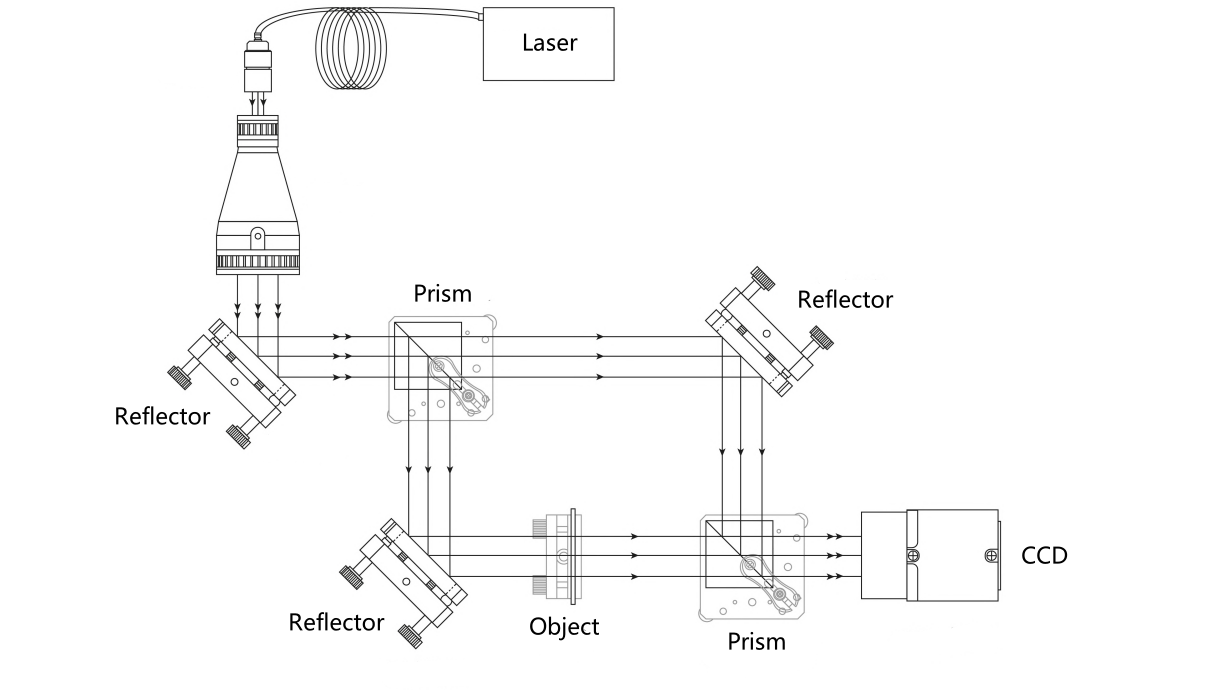
\includegraphics[width=0.4\textwidth]{attachments/fig.illus-5.4.png}
			}
			\caption{\textbf{Light path of computational holography and digital holography}}
		\end{figure*}

	\subsection{Method}
	We first measured the amplitude modulation curve of the SLM by loading images on increasing gray scales.
	Then, using SLM loaded with checker image as object, we measured the distortion in different convex lens imaging systems.
	As for optical information processing, we first investigated Abbe's theory of image formation by studying the one-dimensional grating diffraction, 
	following which we conducted spatial filtering experiments (high-pass, low-pass and band-pass filtering) to realize different optical information processing.
	Finally, we conducted computational holography and digital holography experiments to study the principles of holography.

%%end-------------------Method-----------------------%%

%%begin-------------------Result-----------------------%%
\section{Result}
	\subsection{Amplitude modulation curve of the SLM}
	Amplitude modulation curve of the SLM is shown in Fig. \ref{fig.1.1}. We found that there was a threshold at about 100, 
	before which the SLM did not respond to the change of gray scale and the output light power remained close to zero. 
	After the threshold, as the gray scale increased, the output light power increased rapidly, and finally reached saturation at about 255.
	
	This threshold phenomenon can be explained by the mechanism of the TTNLC-SLM responding to the control voltage. 
	As previously introduced (Eq. \ref{eq.1.3}), there exists a threshold control voltage $V_c$, which is the minimal required voltage to twist the liquid crystal molecules.
	If $V_s < V_c$, there is no modulation effect as the voltage is not sufficient to twist the molecules; As the voltage increases, the twisting effect of the electric field increases, thus the transmissivity decreases predominantly.
	As the gray scale of the loaded image increases, the control voltage decreases. Once the control voltage is below the threshold, the SLM does not respond to the change of gray scale.

	\begin{figure*}[htbp]
		\centering
		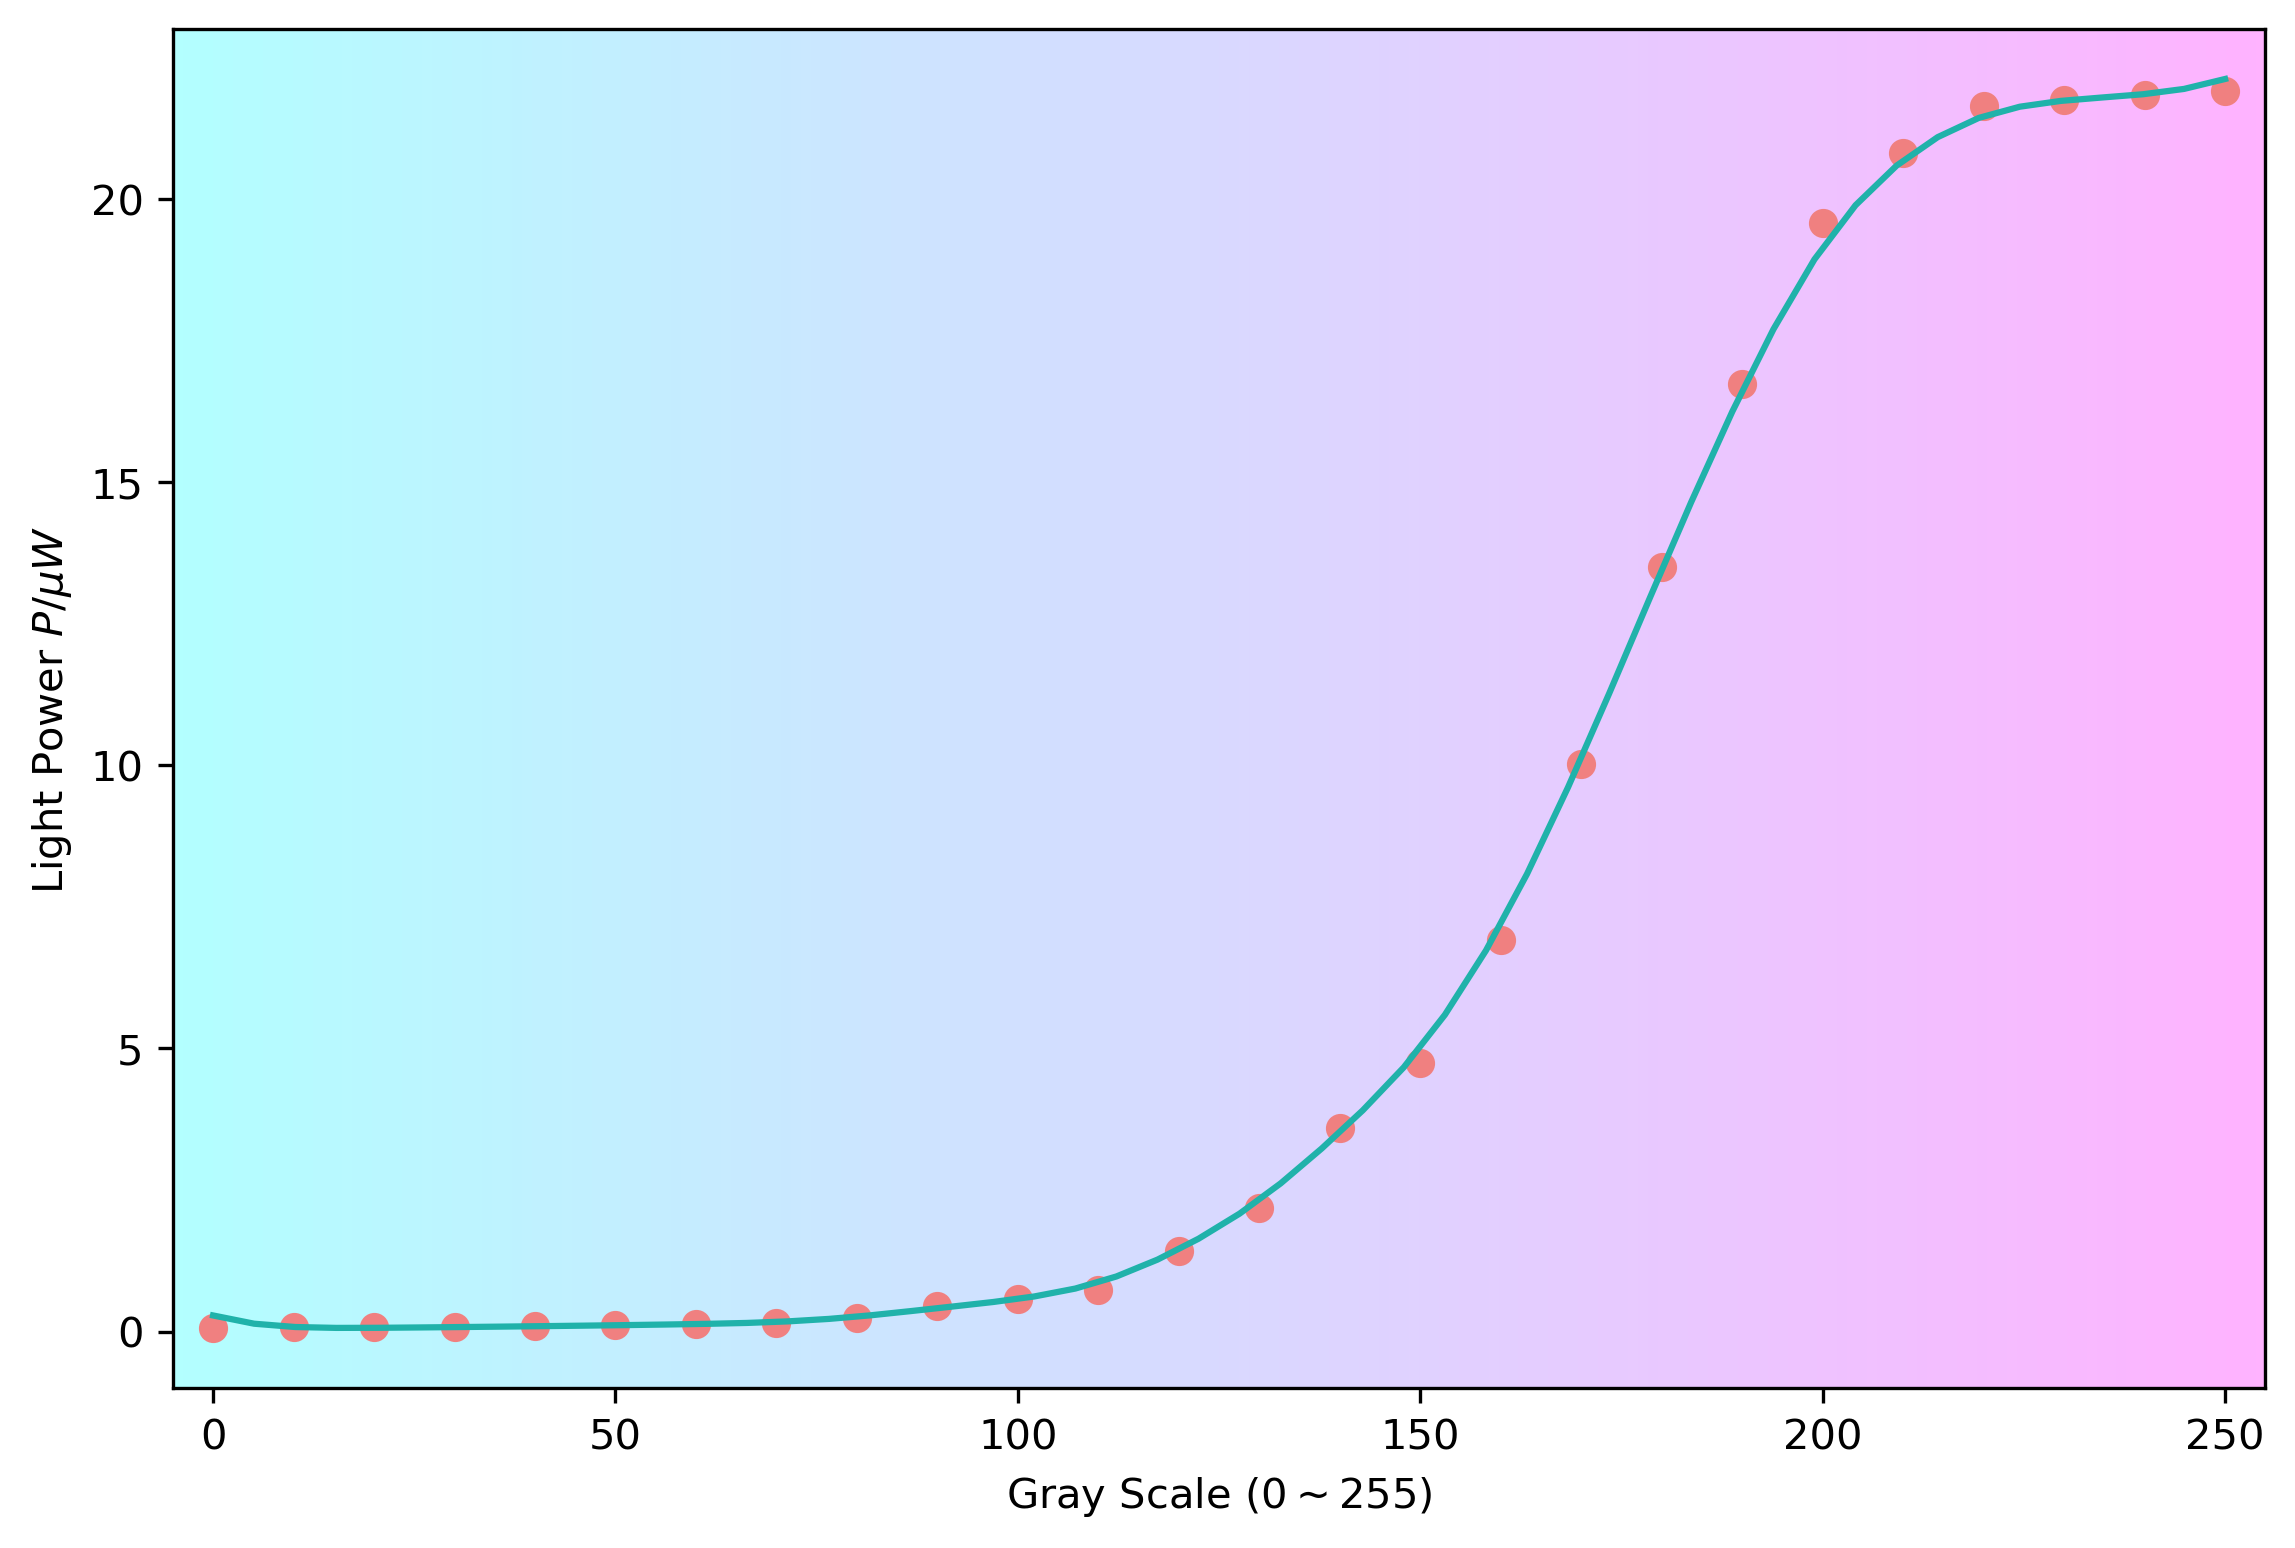
\includegraphics[width=0.6\textwidth]{attachments/fig.1.1.png}
		\caption{\textbf{Amplitude modulation curve of the SLM}}
		\label{fig.1.1}
	\end{figure*}

	\subsection{Distortion of convex lens imaging system}
	In this experiment we measured the distortion of convex lens imaging system with focus of $50, 70, 150 mm$ when the amplification $\beta$ was set as $\frac{1}{6}, \frac{1}{4}, \frac{1}{2}, 2, 4$.
	
	The results are shown in Fig. \ref{fig.2.1} and summarized in Tab. \ref{tab.2.1} (Details in Supplementary Information).
	
	We found that
		\begin{enumerate}[label=\arabic*.]
			\item Distortions in different orientations ($X$, $Y$, $+45^o$) generally remain constant, which means that the system is spherically symmetric.
			\item For the same amplification, for shrinking system ($\beta<0$), as the focus of the lens decreases, the distortion of the convex lens imaging system increases.
			\item For the same focus, for the shrinking system ($\beta<0$), as the amplification decreases, the distortion of the convex lens imaging system increases.
			\item For the same focus, for the expanding system ($\beta>0$), as the amplification increases, the distortion of the convex lens imaging system increases.
		\end{enumerate}

	These phenomena can be explained by the optical angle $\theta = \frac{\beta Y}{s_2}$, which represents the "off-axis" degree. 
	As previously discussed, distortion of the convex lens imaging system is a non-paraxial effect.
	Generally, as $\theta$ increases, which means that the edge (sampling point) is relatively farther away from the axis, the distortion effect becomes more prominent.

	As for the type of distortion, we found that Fig. \ref{fig.2.1}, Fig. \ref{fig.2.6} and Fig. \ref{fig.2.7} are barrel distortion, while the others are pincushion distortion.
	We haven't found a solid conclusion about the reason of different types of distortion.

	\begin{figure*}[htbp]
		\centering		
		\subfloat[$f=150, \beta = \frac{1}{4}$]{\label{fig.2.1}
		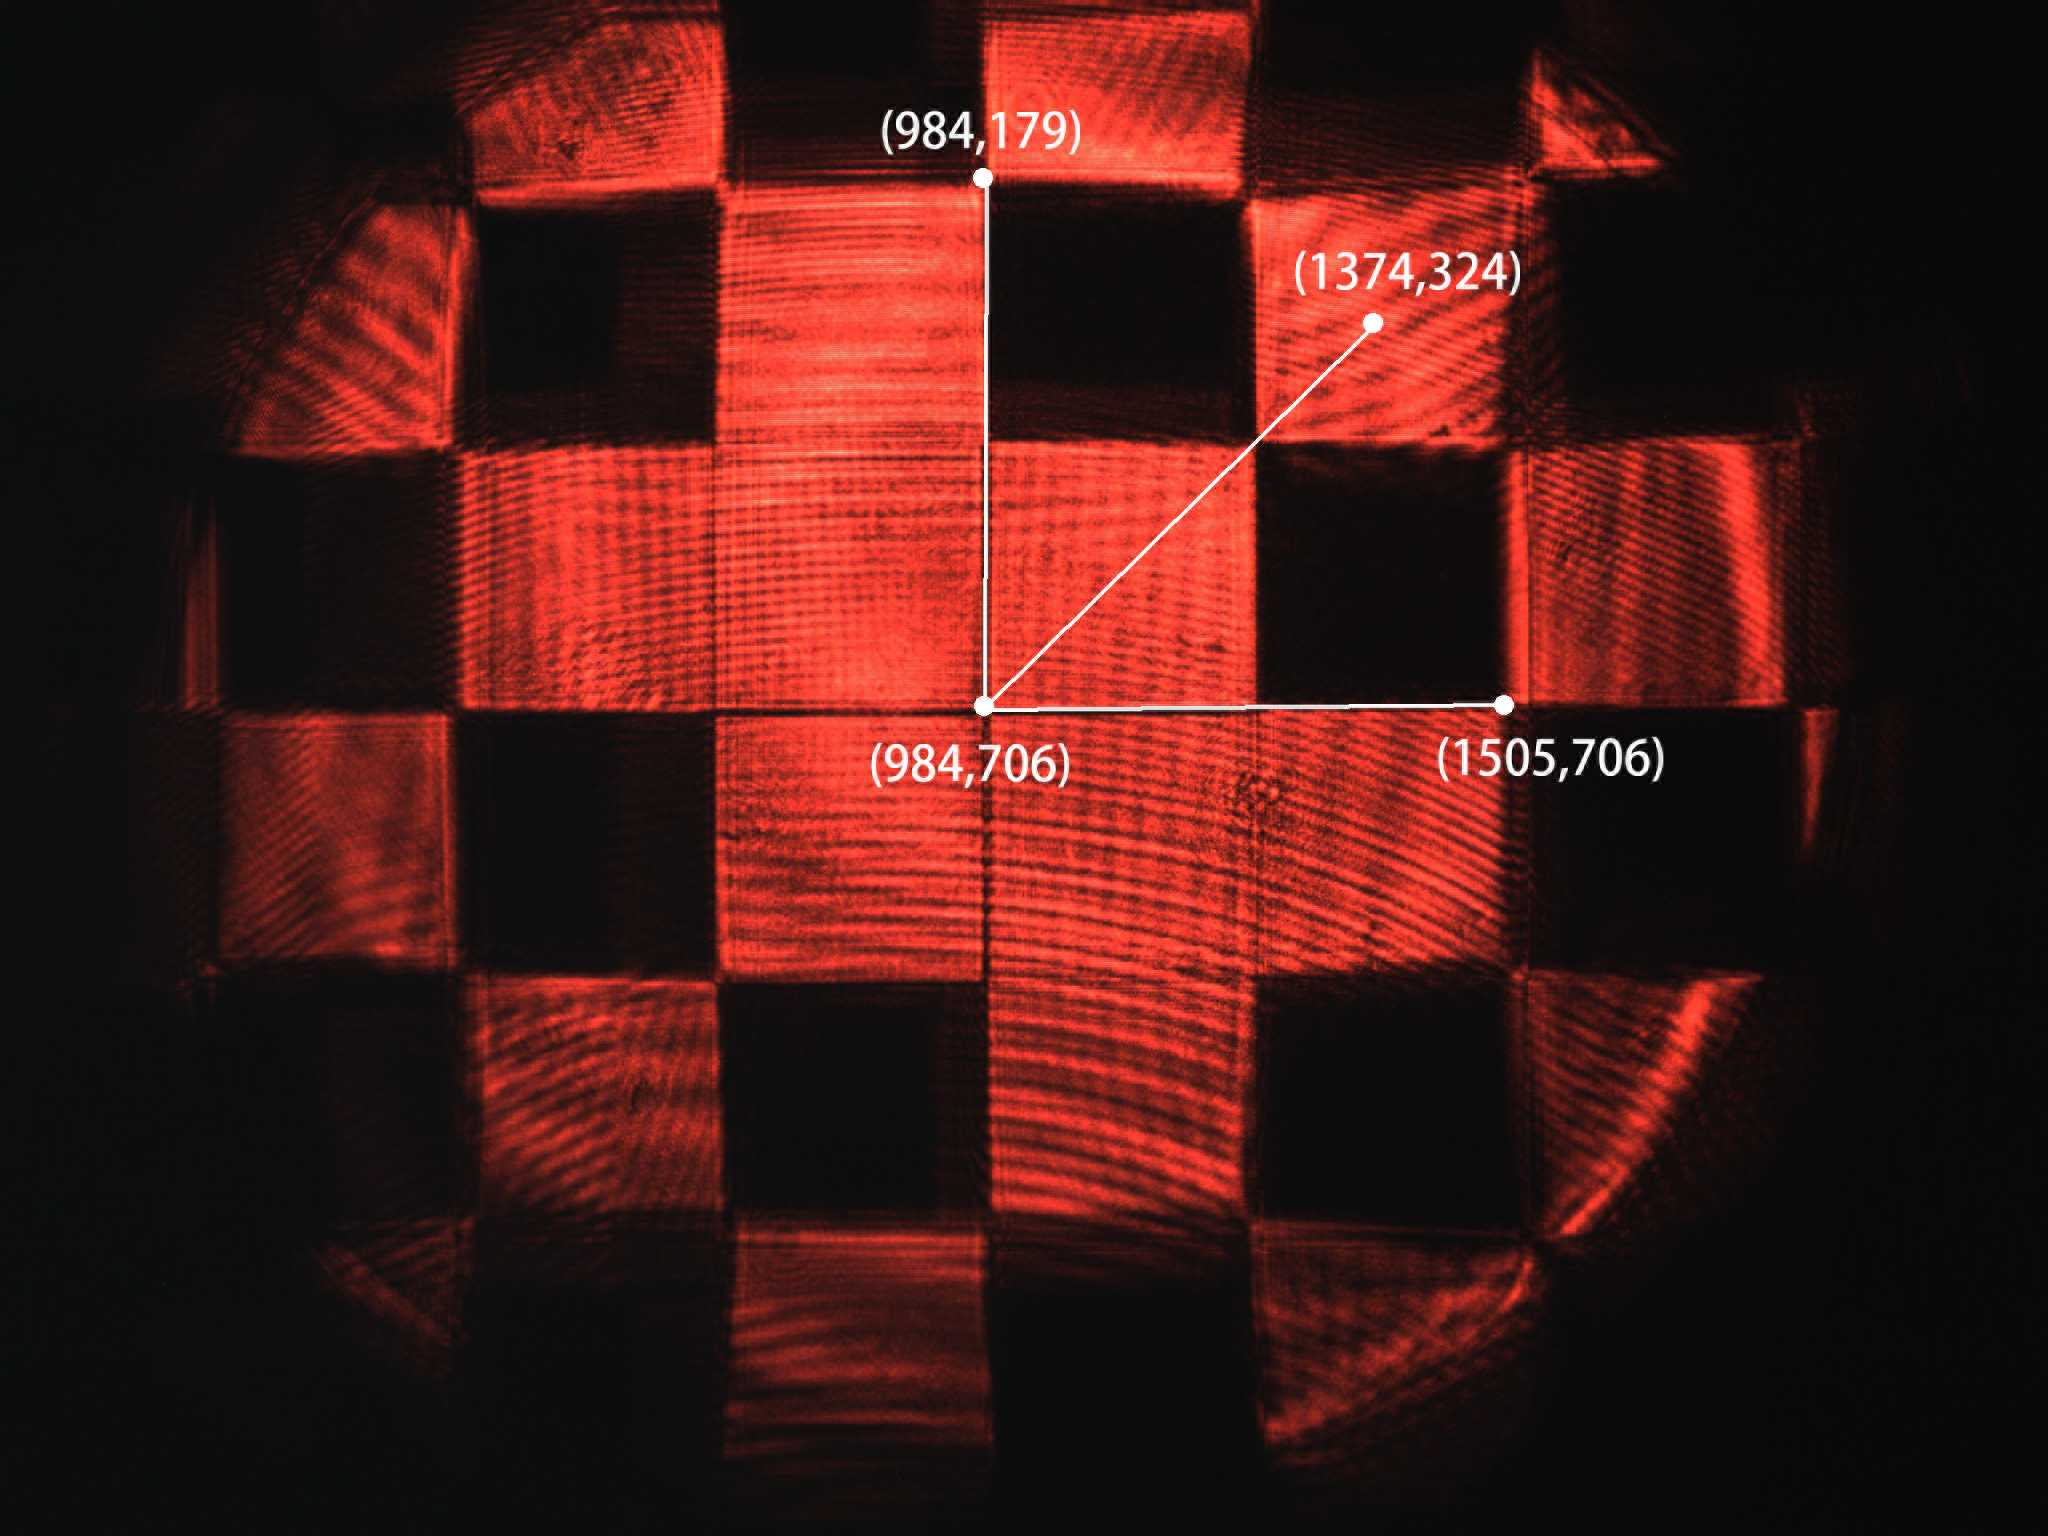
\includegraphics[width=0.24\textwidth]{attachments/fig.2.1.jpg}
		}
		\subfloat[$f=70, \beta = \frac{1}{4}$]{\label{fig.2.2}
		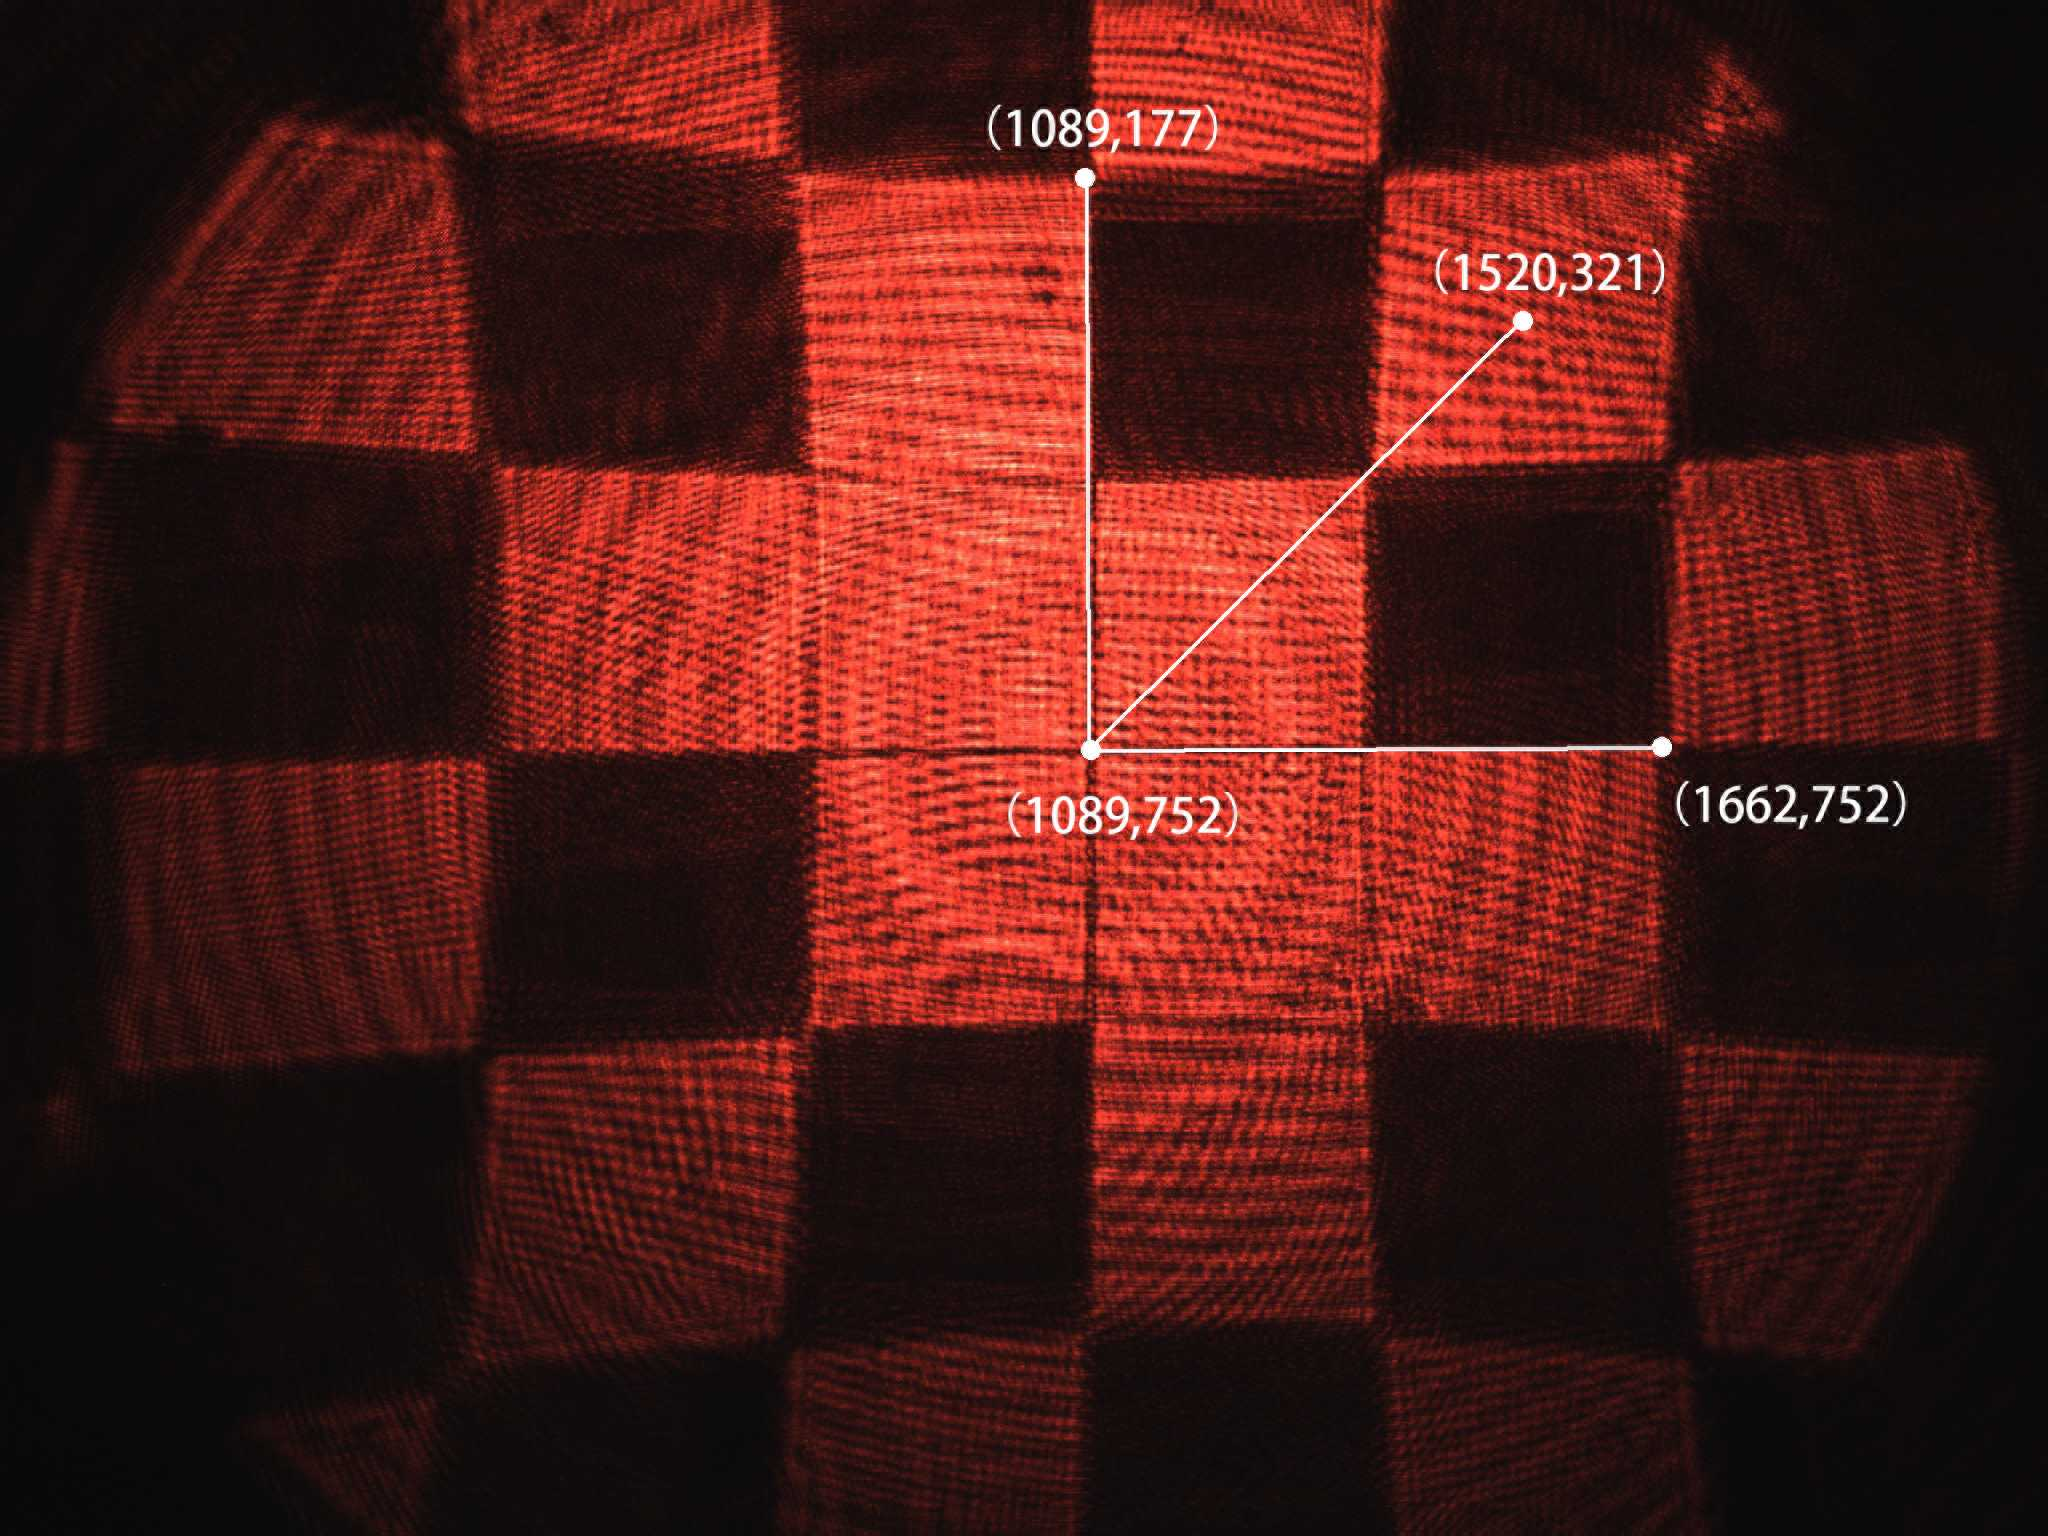
\includegraphics[width=0.24\textwidth]{attachments/fig.2.2.jpg}
		}
		\subfloat[$f=50, \beta = \frac{1}{4}$]{\label{fig.2.3}
		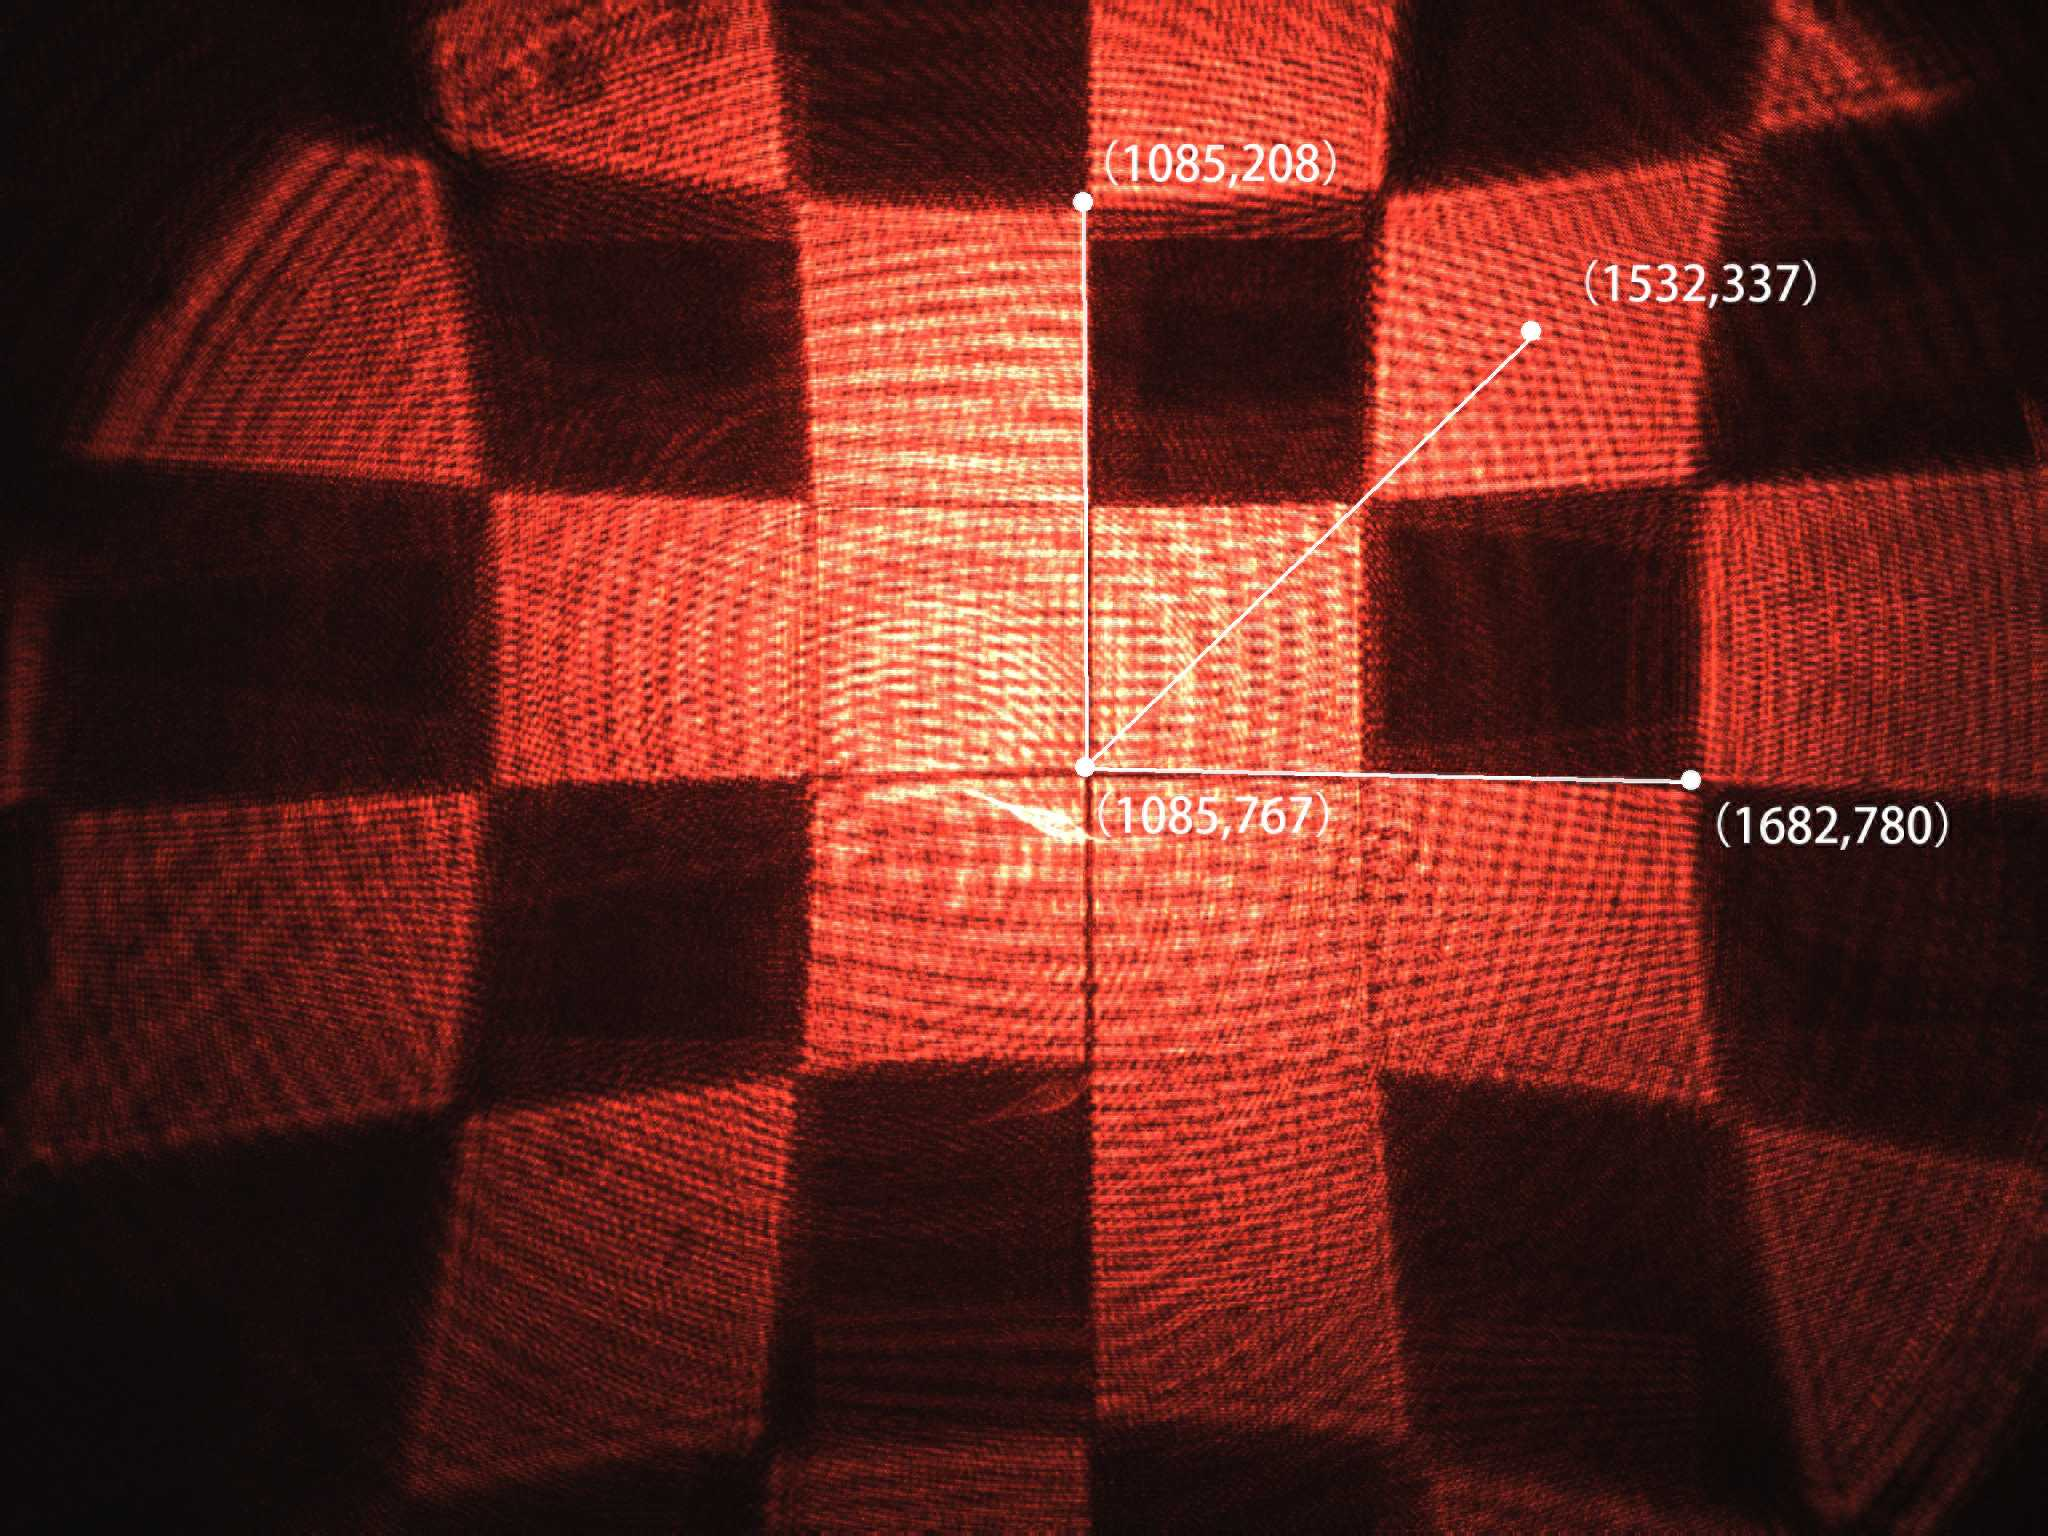
\includegraphics[width=0.24\textwidth]{attachments/fig.2.3.jpg}
		}

		\subfloat[$f=70, \gamma = \frac{1}{2}$]{\label{fig.2.4}
		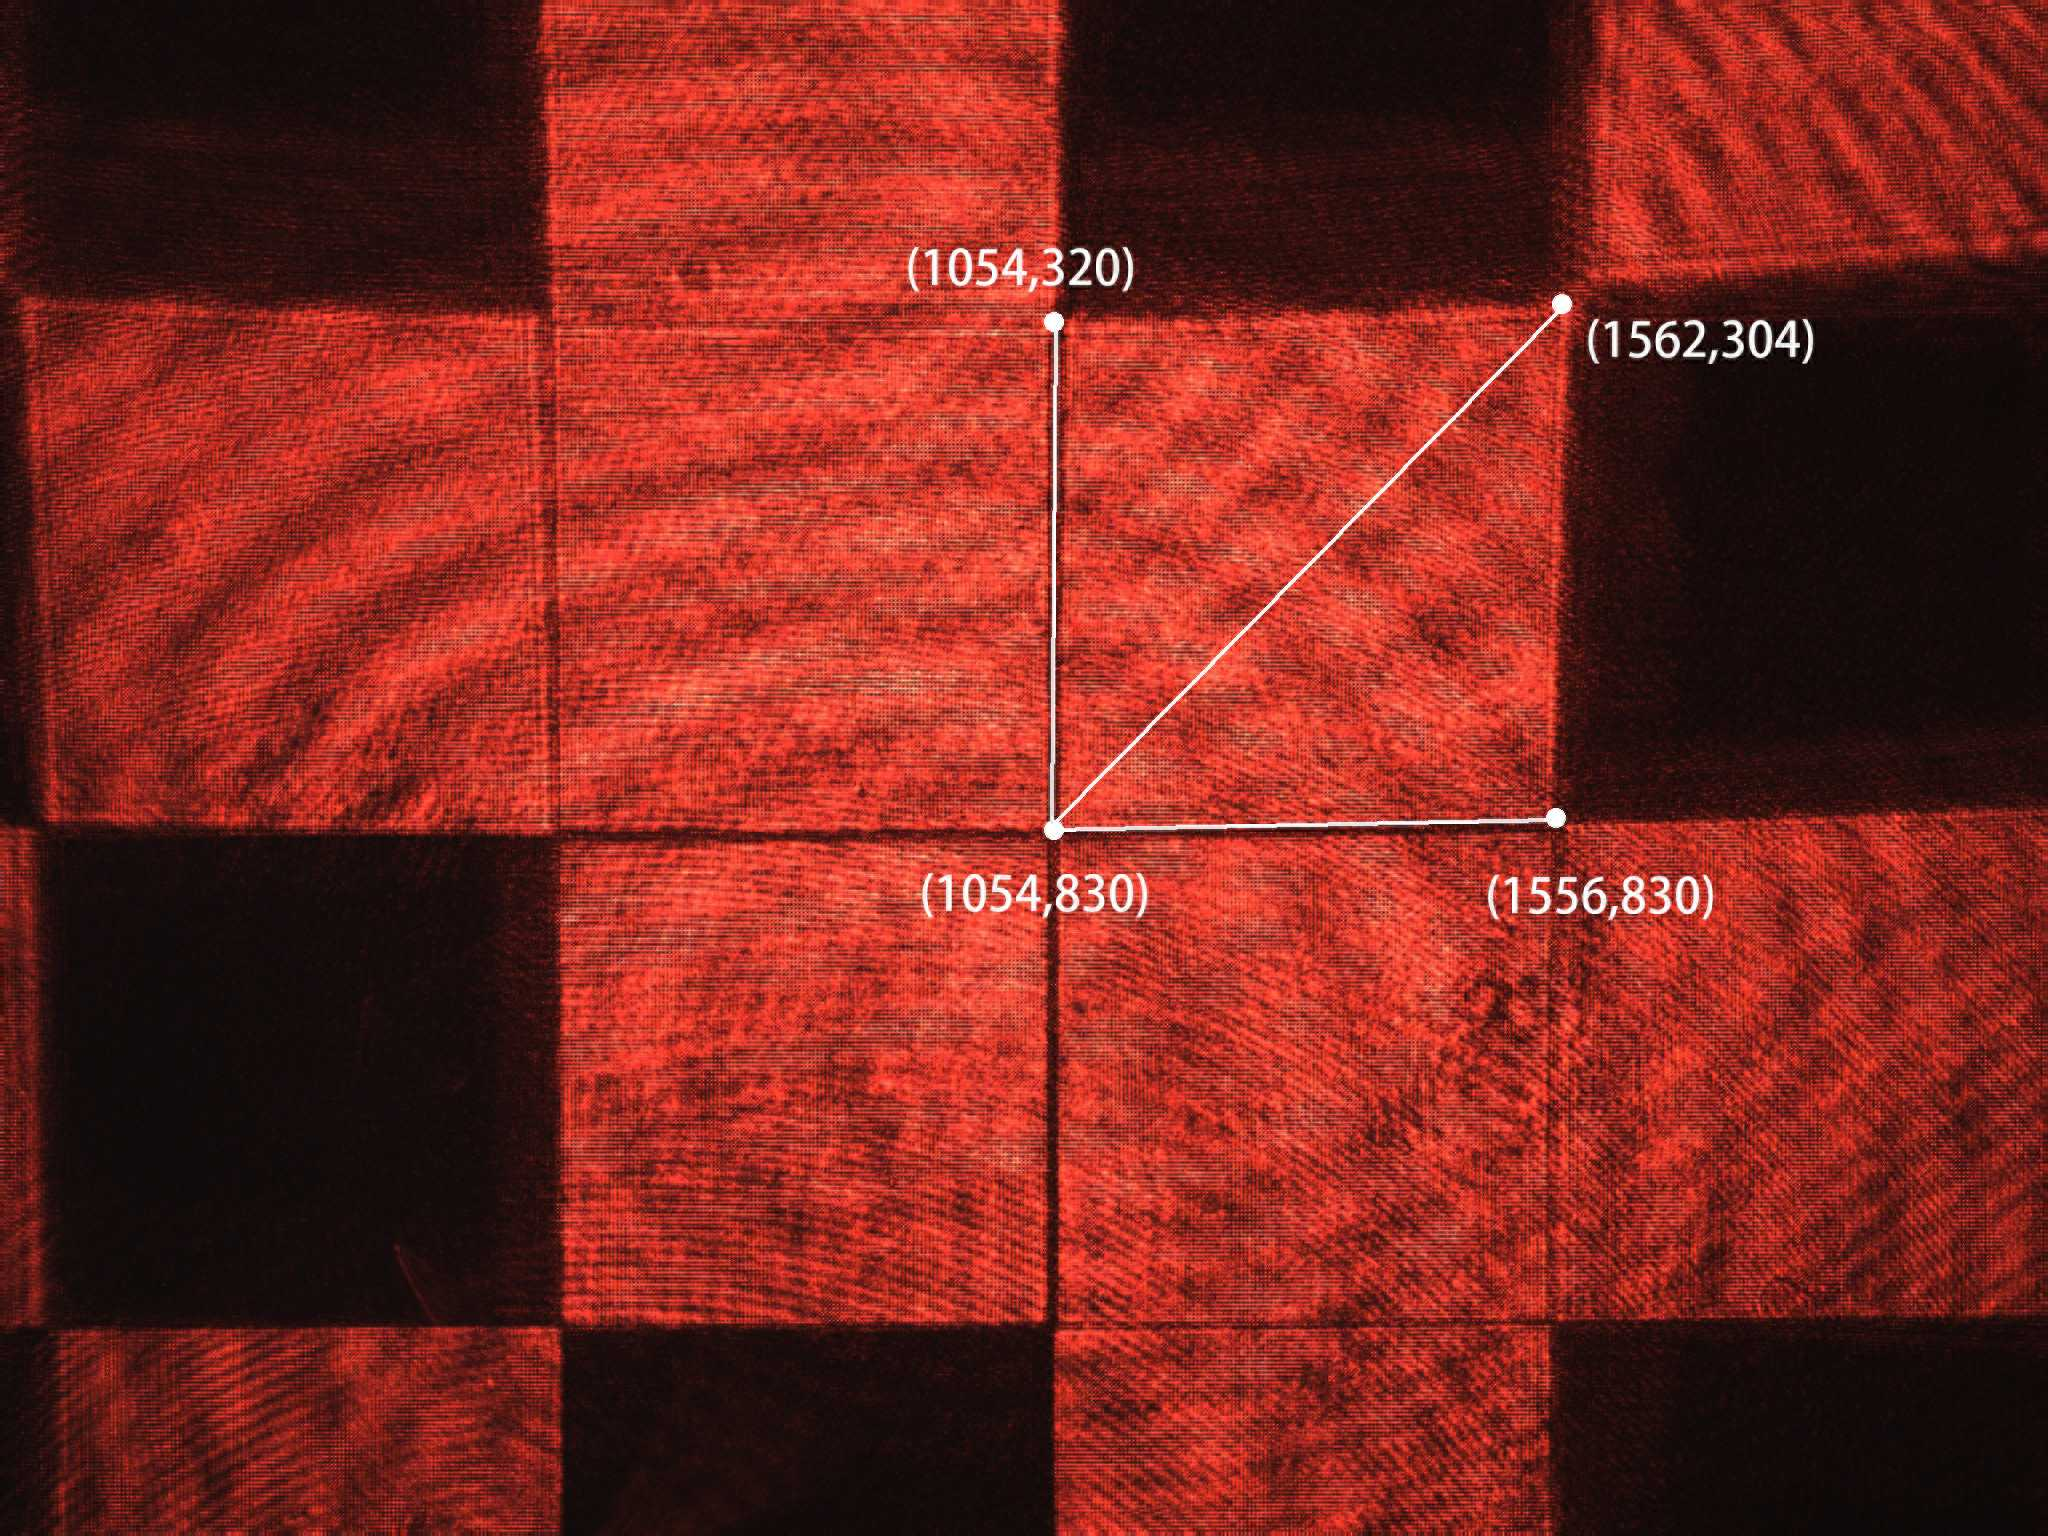
\includegraphics[width=0.24\textwidth]{attachments/fig.2.4.jpg}
		}
		\subfloat[$f=70, \gamma = \frac{1}{6}$]{\label{fig.2.5}
		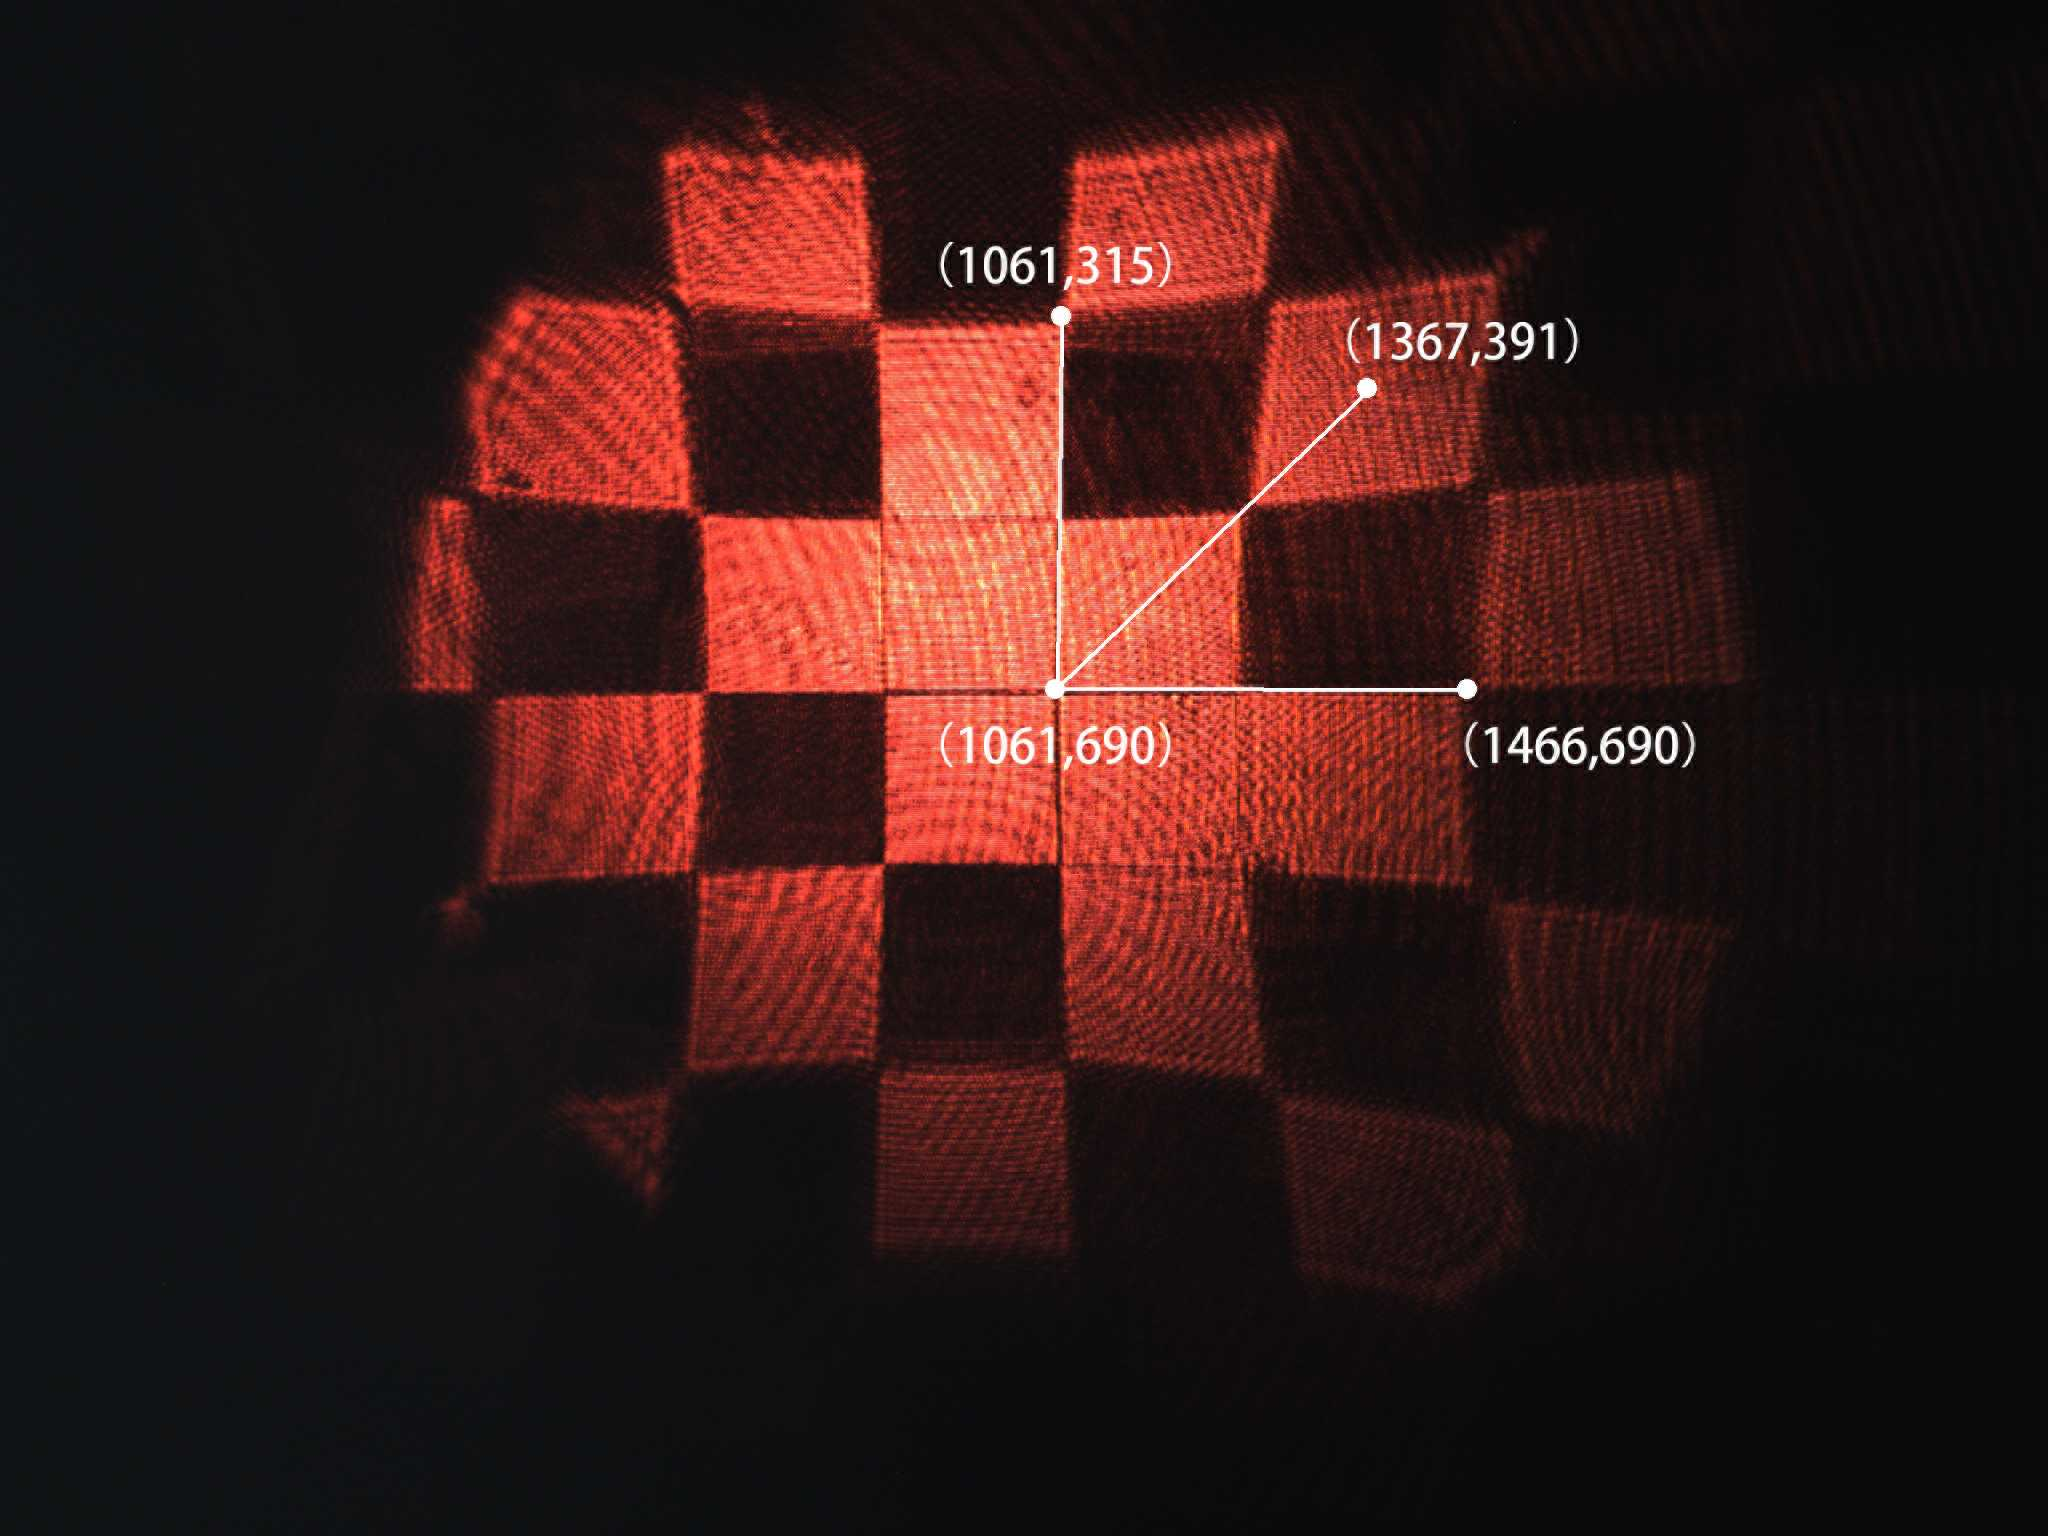
\includegraphics[width=0.24\textwidth]{attachments/fig.2.5.jpg}
		}
		\subfloat[$f=70, \gamma = 2$]{\label{fig.2.6}
		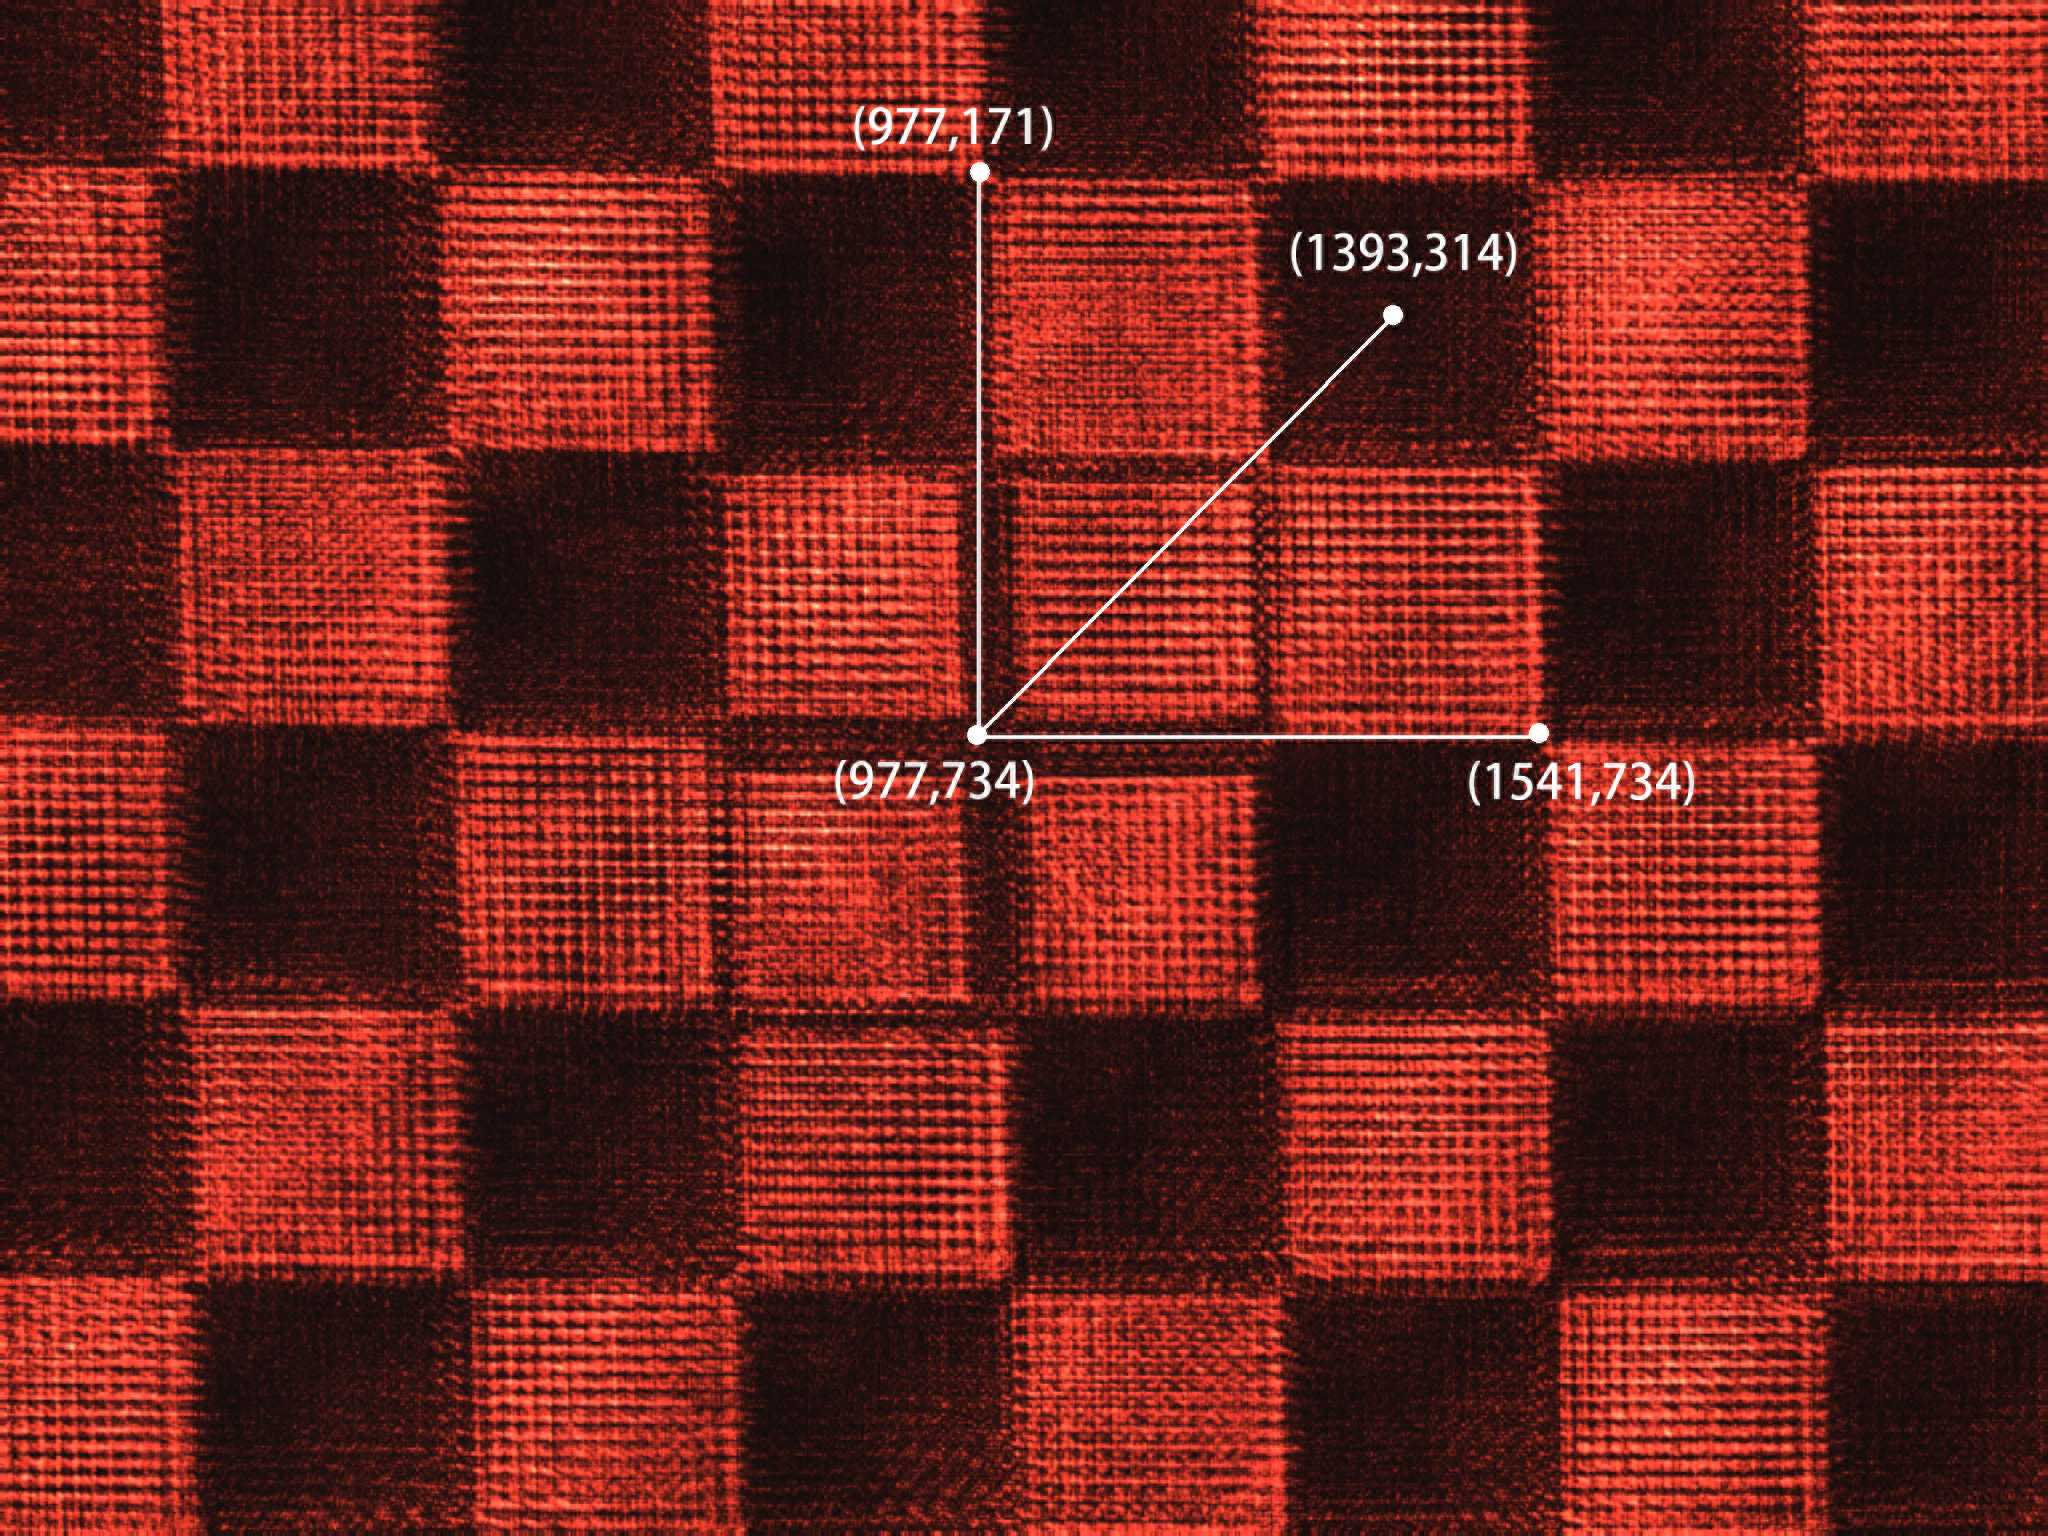
\includegraphics[width=0.24\textwidth]{attachments/fig.2.6.jpg}
		}
		\subfloat[$f=70, \gamma = 4$]{\label{fig.2.7}
		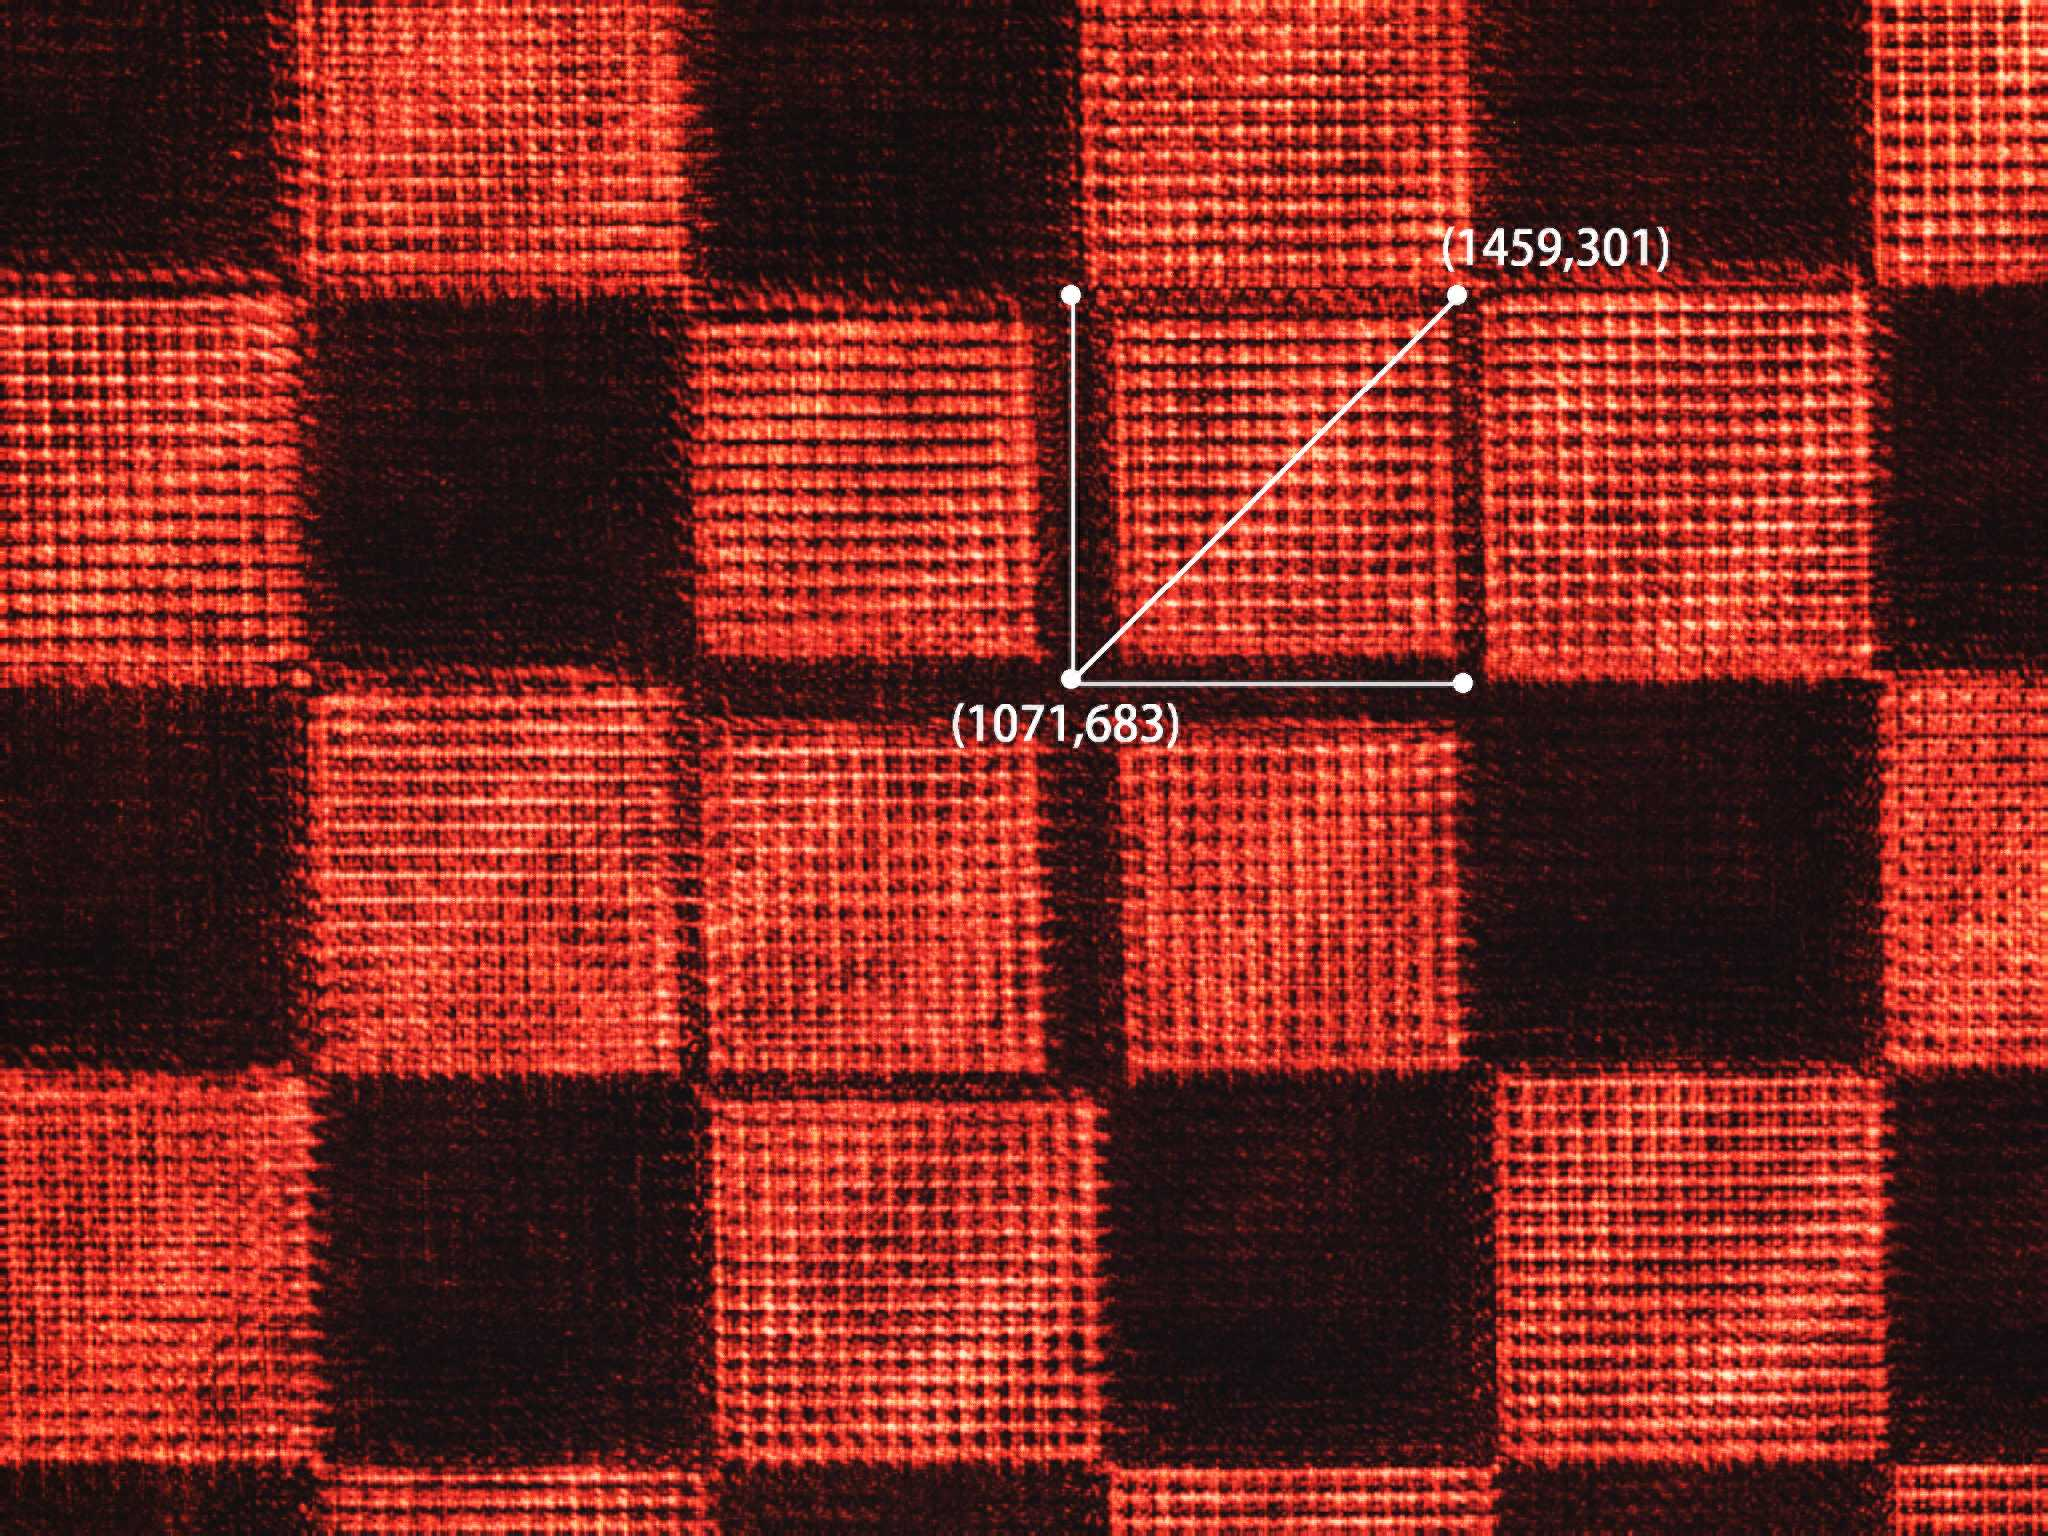
\includegraphics[width=0.24\textwidth]{attachments/fig.2.7.jpg}
		}
		\caption{\textbf{Distortion of convex lens imaging system}}
	\end{figure*}

	\begin{table*}[htbp]
		\centering
		\caption{\textbf{Distortion of convex lens imaging system}}
		\label{tab.2.1}
			\begin{tabular}{llllllll}
				\toprule
				$f/mm$ &  $\beta$	&$s_2$	&$\theta$ &$X$ &$Y$ &$45^o, x\ comp.$ &$45^o, y\ comp.$ \\
				\midrule
				150 & 0.250 & 187.50 &  2.218667 &   0.19\% &   1.35\% &   0.00\% &  -2.05\% \\
				70 & 0.250 &  87.50 &  4.754286 &  10.19\% &  10.58\% &  10.51\% &  10.51\% \\
				50 & 0.250 &  62.50 &  6.656000 &  14.81\% &   7.50\% &  14.62\% &  10.26\% \\
				70 & 0.500 & 105.00 &  7.923810 &  -3.46\% &  -1.92\% &  -2.31\% &   1.15\% \\
				70 & 0.166 &  81.64 &  2.246604 &  17.30\% &   8.61\% &  18.16\% &  15.46\% \\
				70 & 2.000 & 105.00 & 31.695238 &   8.46\% &   8.27\% &   6.67\% &   7.69\% \\
				70 & 4.000 &  87.50 & 76.068571 & -25.38\% & -26.54\% & -25.38\% & -26.54\% \\
				\bottomrule
			\end{tabular}
	\end{table*}

	\subsection{Optical information processing}
		\subsubsection{Abbe's theory of image formation}
		"4f system"(Fig. \ref{fig.illus-4.1}) is the most common light path in optical information processing. 
		To verify the effectiveness of the single-lens system (Fig. \ref{fig.illus-4.2}) and SLM in optical information processing as well as investigating the principles of Abbe's theory,
		we first built the "4f system" and used one-dimensional grating as object to conduct the diffraction experiments. 
		The spatial spectrum (Fig. \ref{fig.3.1.1.1}) on the Fourier's plane $P_2$ and the diffraction fringes (Fig. \ref{fig.3.1.1.2}) on the image plain $P_3$ was obtained, respectively.
		We also used optical aperture to filter the spatial spectrum (Only allow 0, 1, 2 order spot to pass, respectively) and investigated the changes of the diffraction patterns (Fig. \ref{fig.3.1.2.1}, \ref{fig.3.1.2.2}, \ref{fig.3.1.2.3}).
		Then, we repeated this experiment on the single-lens system using SLM loaded with 128T grating image (Fig. \ref{fig.3.2.0}) as object. 
		The spatial spectrum (Fig. \ref{fig.3.2.1.1}), the diffraction fringes (Fig. \ref{fig.3.2.1.2}) and changes in the diffraction patterns (Fig. \ref{fig.3.2.2.1}, \ref{fig.3.2.2.2}) were also obtained.
		Additionally, we used circular aperture to filter the spatial spectrum (Fig. \ref{fig.3.2.2.3}).

		\begin{figure*}[htbp]
			\centering		
			\subfloat[The spatial spectrum]{\label{fig.3.1.1.1}
			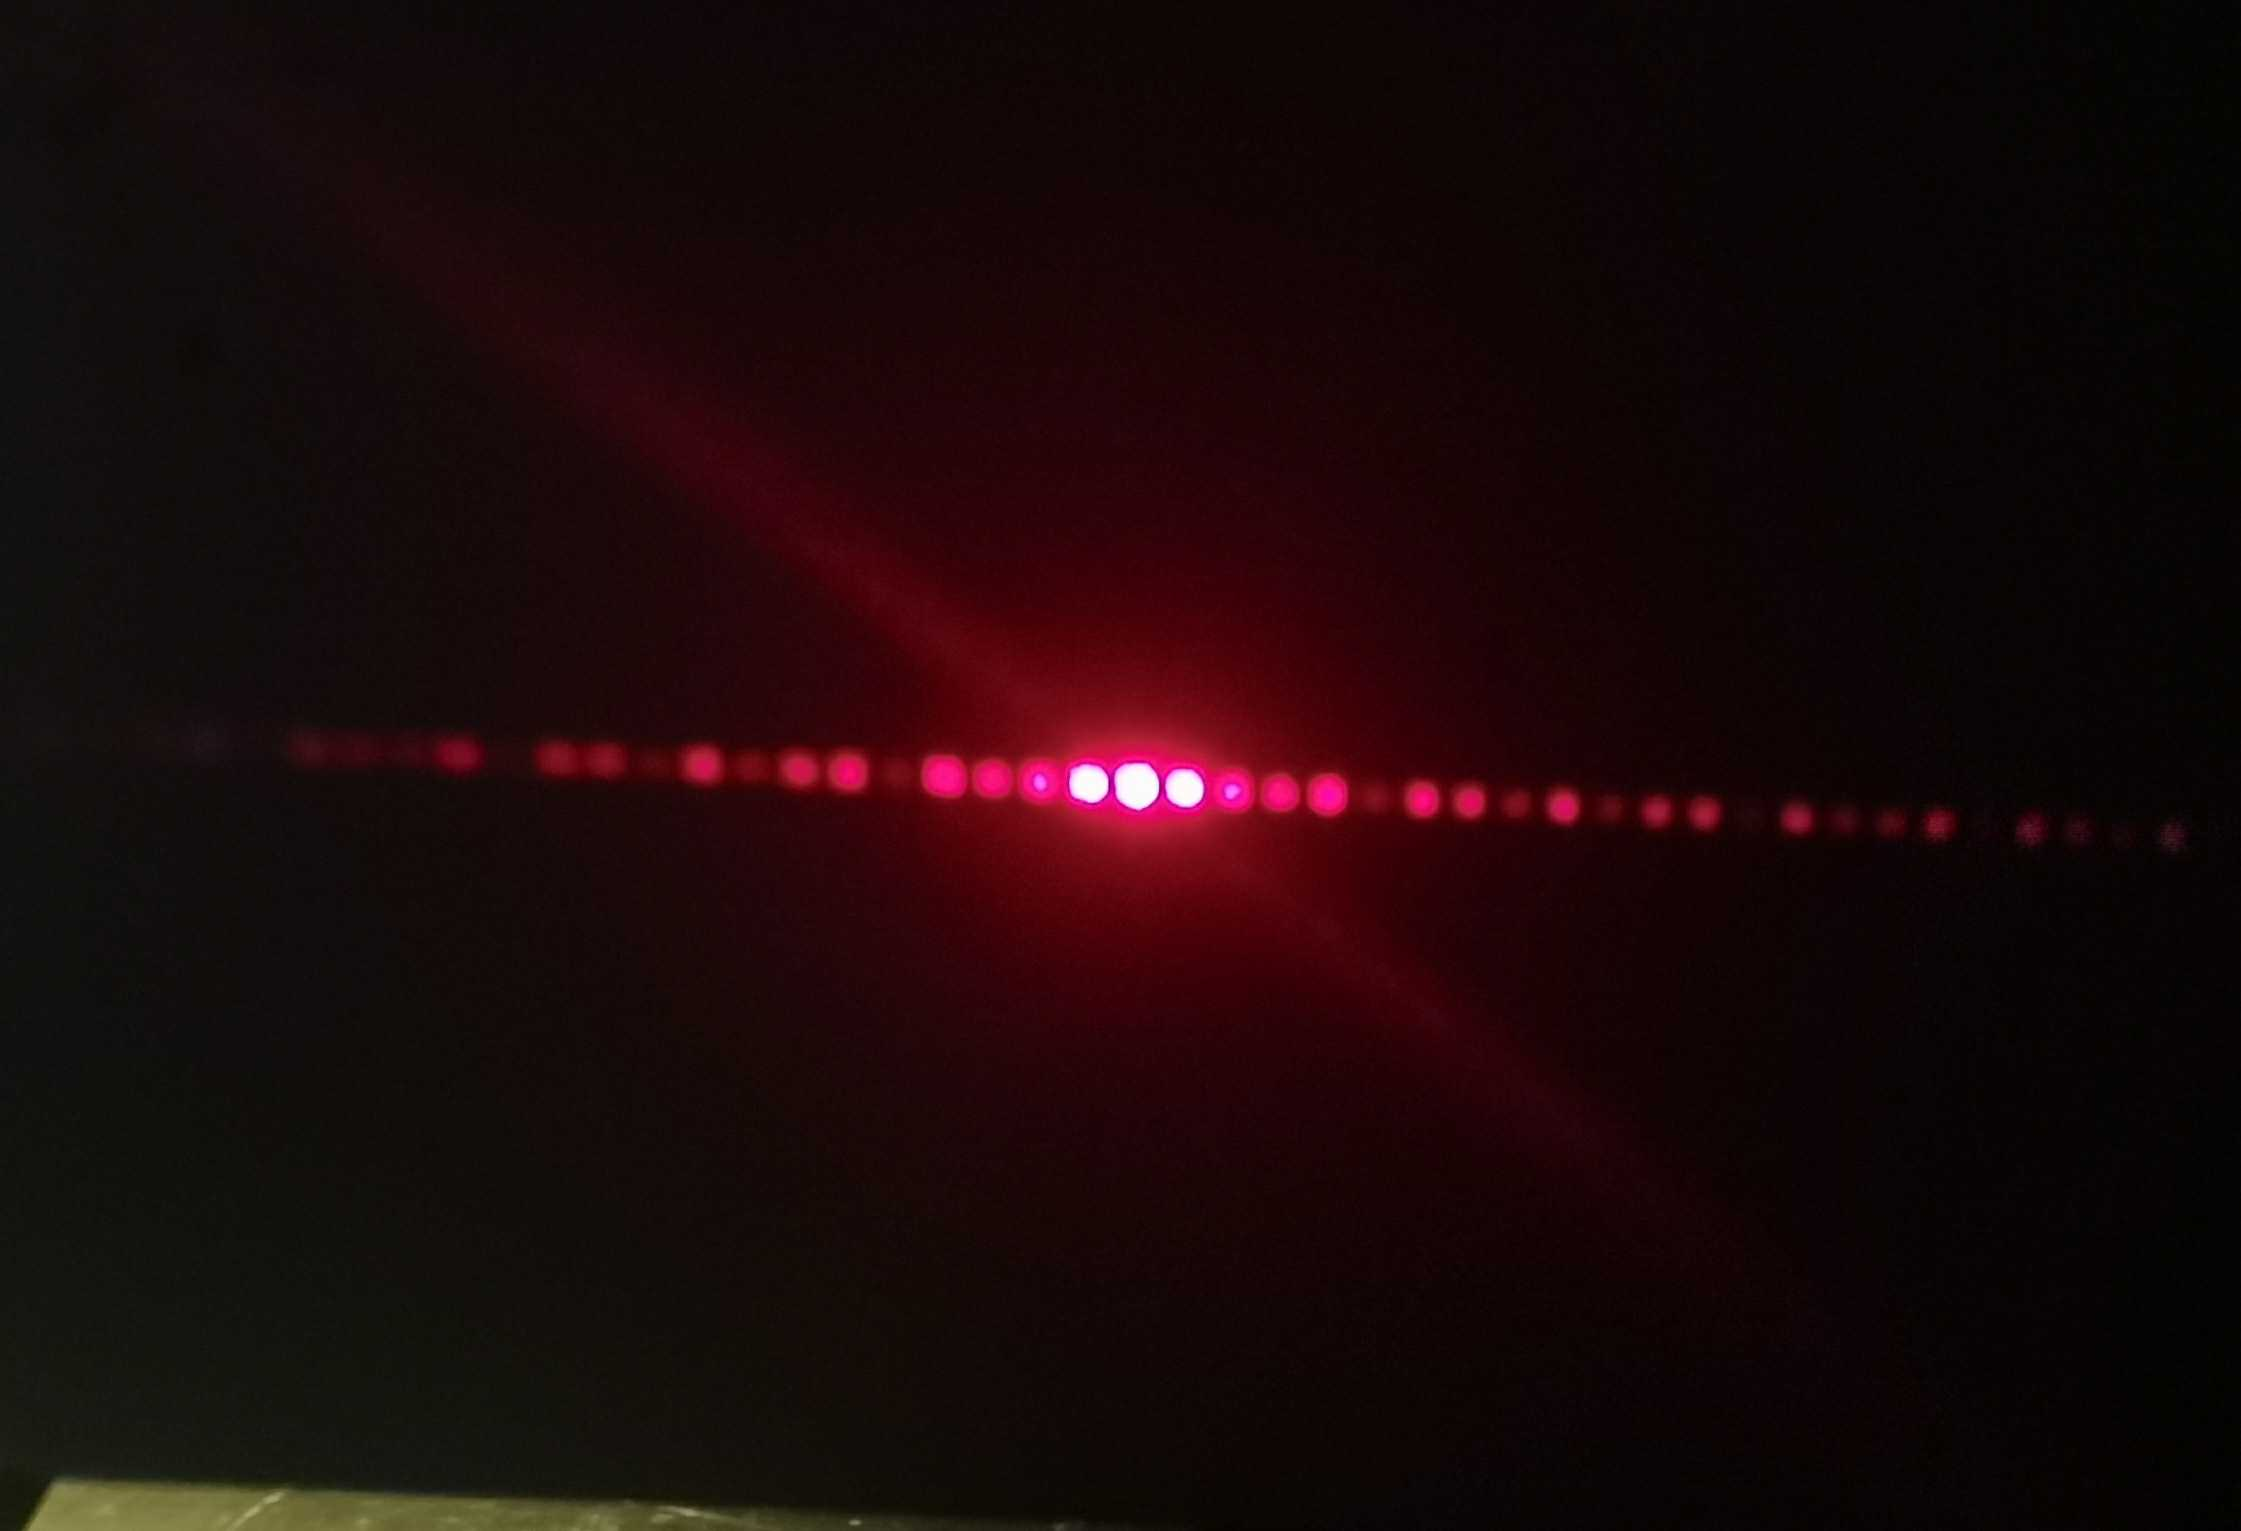
\includegraphics[width=0.3\textwidth]{attachments/fig.3.1.1.1.jpg}
			}
			\subfloat[The diffraction fringes]{\label{fig.3.1.1.2}
			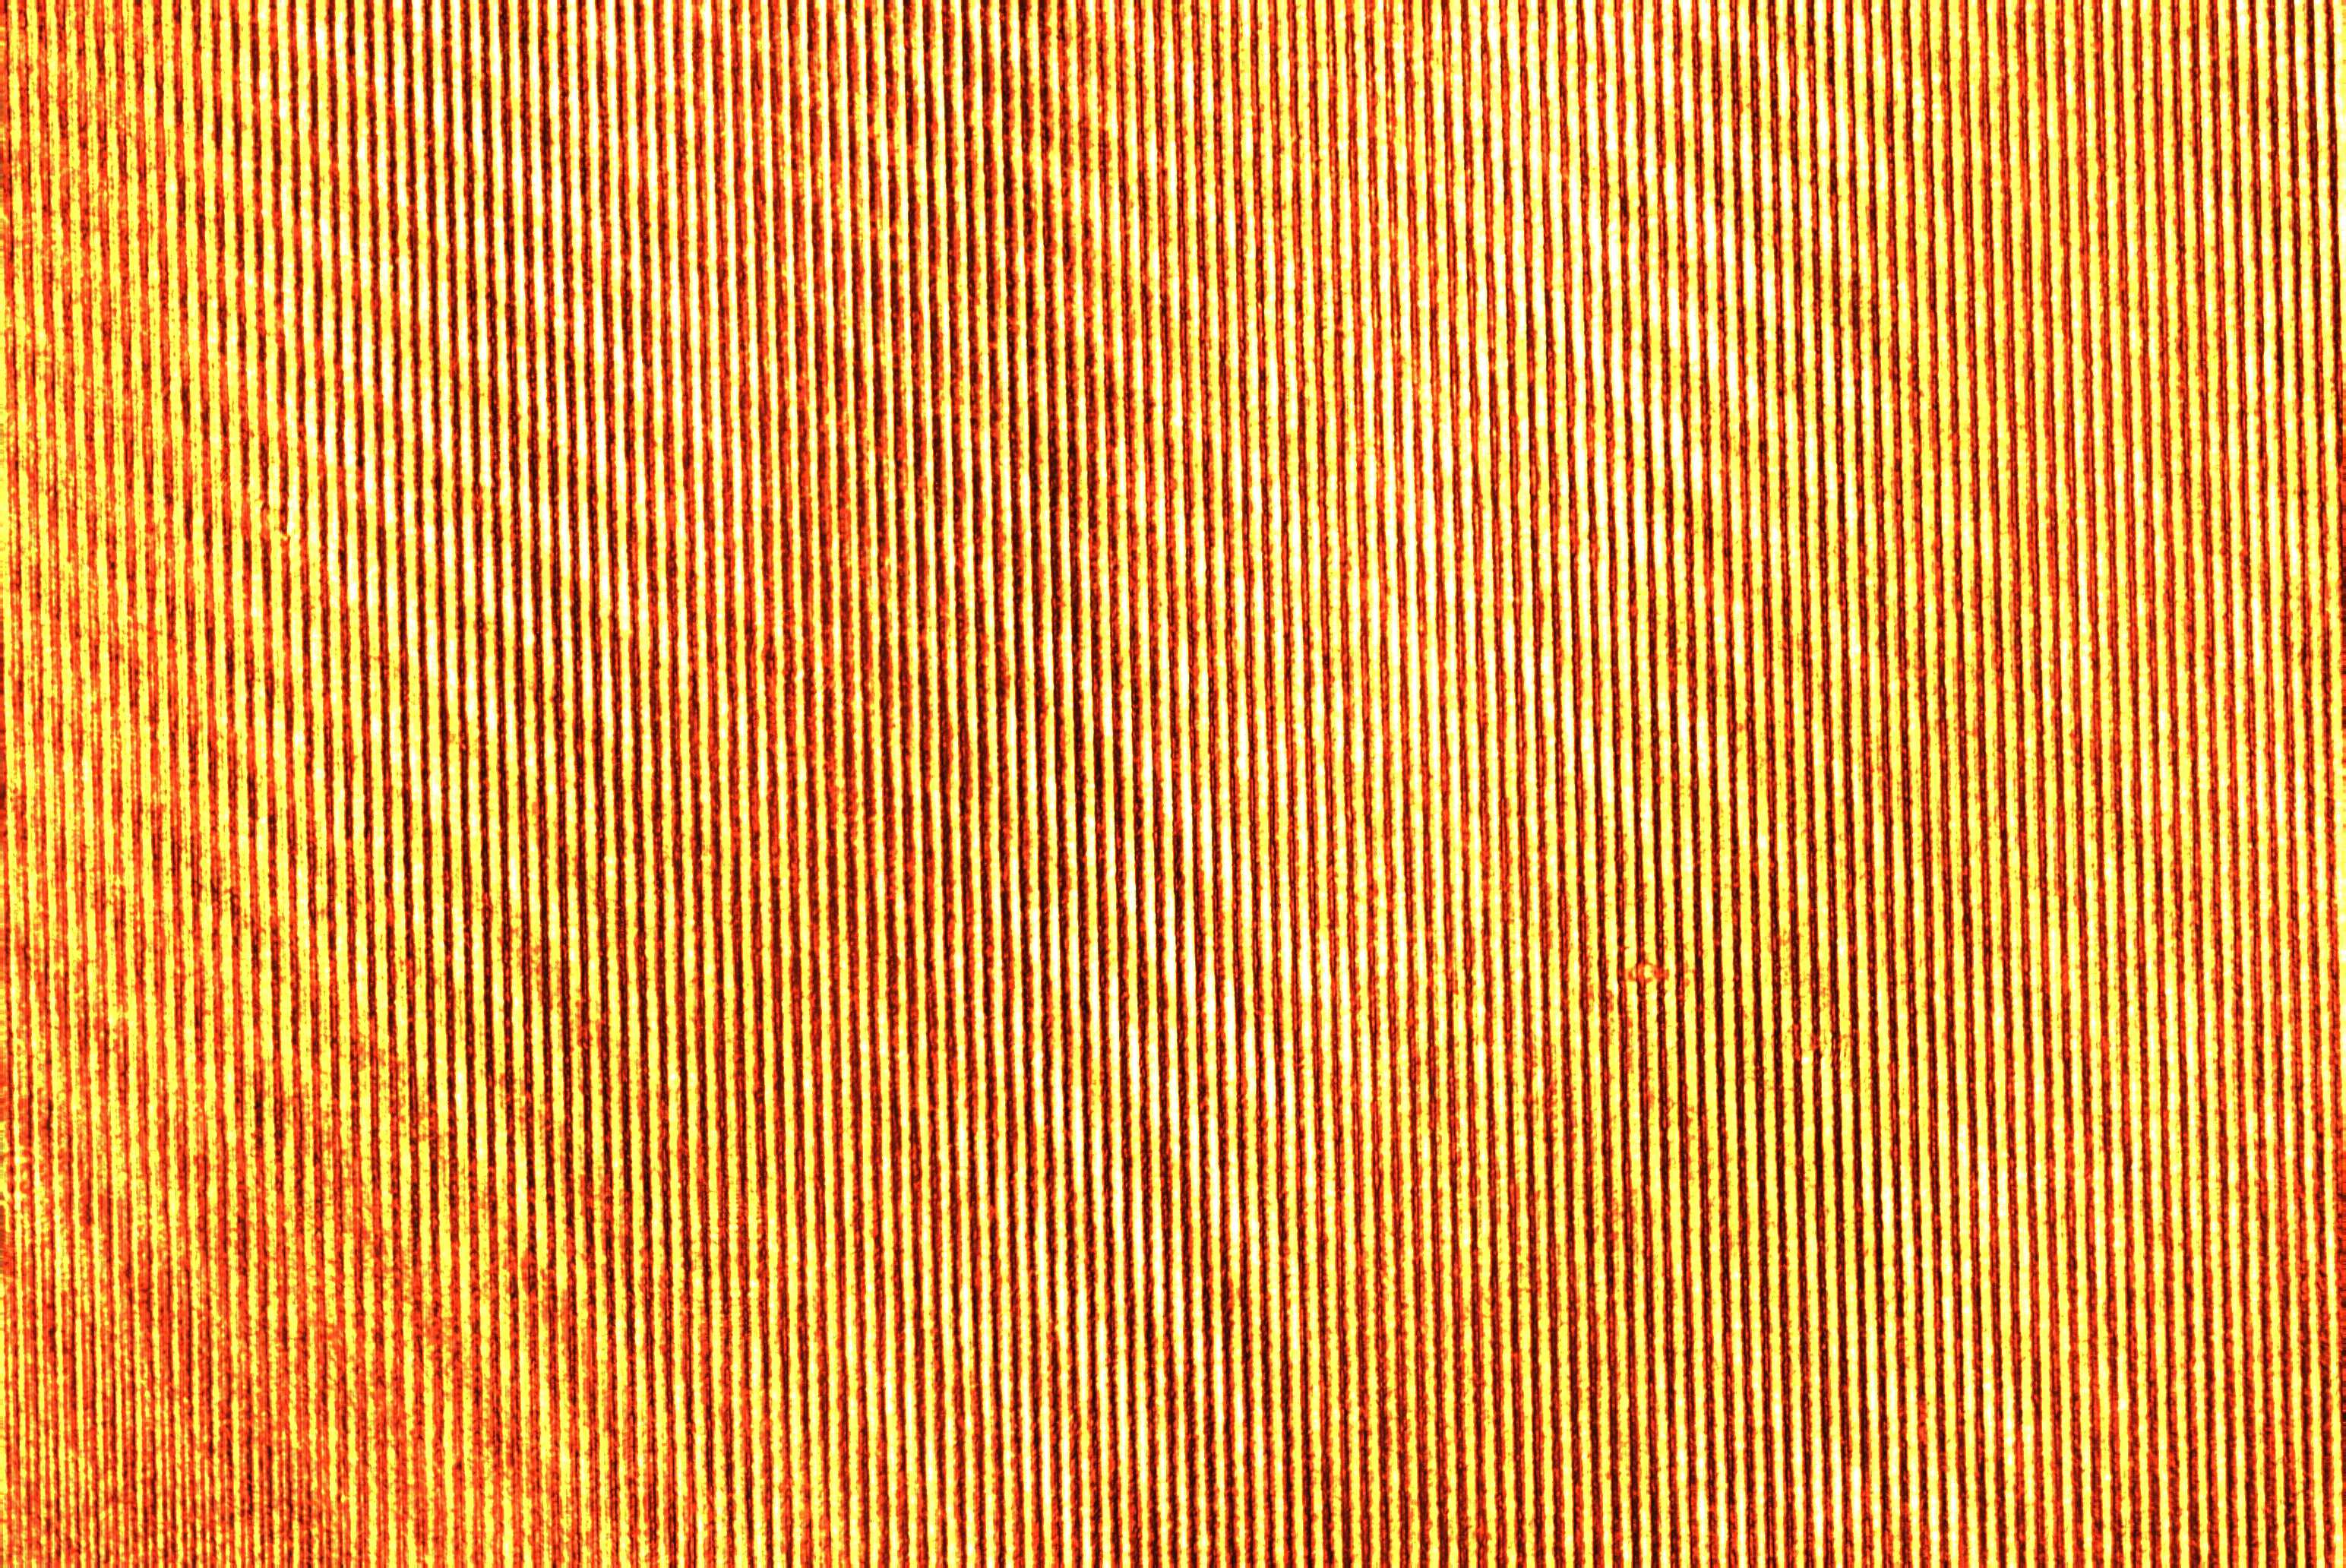
\includegraphics[width=0.3\textwidth]{attachments/fig.3.1.1.2.jpg}
			}

			\subfloat[0 order]{\label{fig.3.1.2.1}
			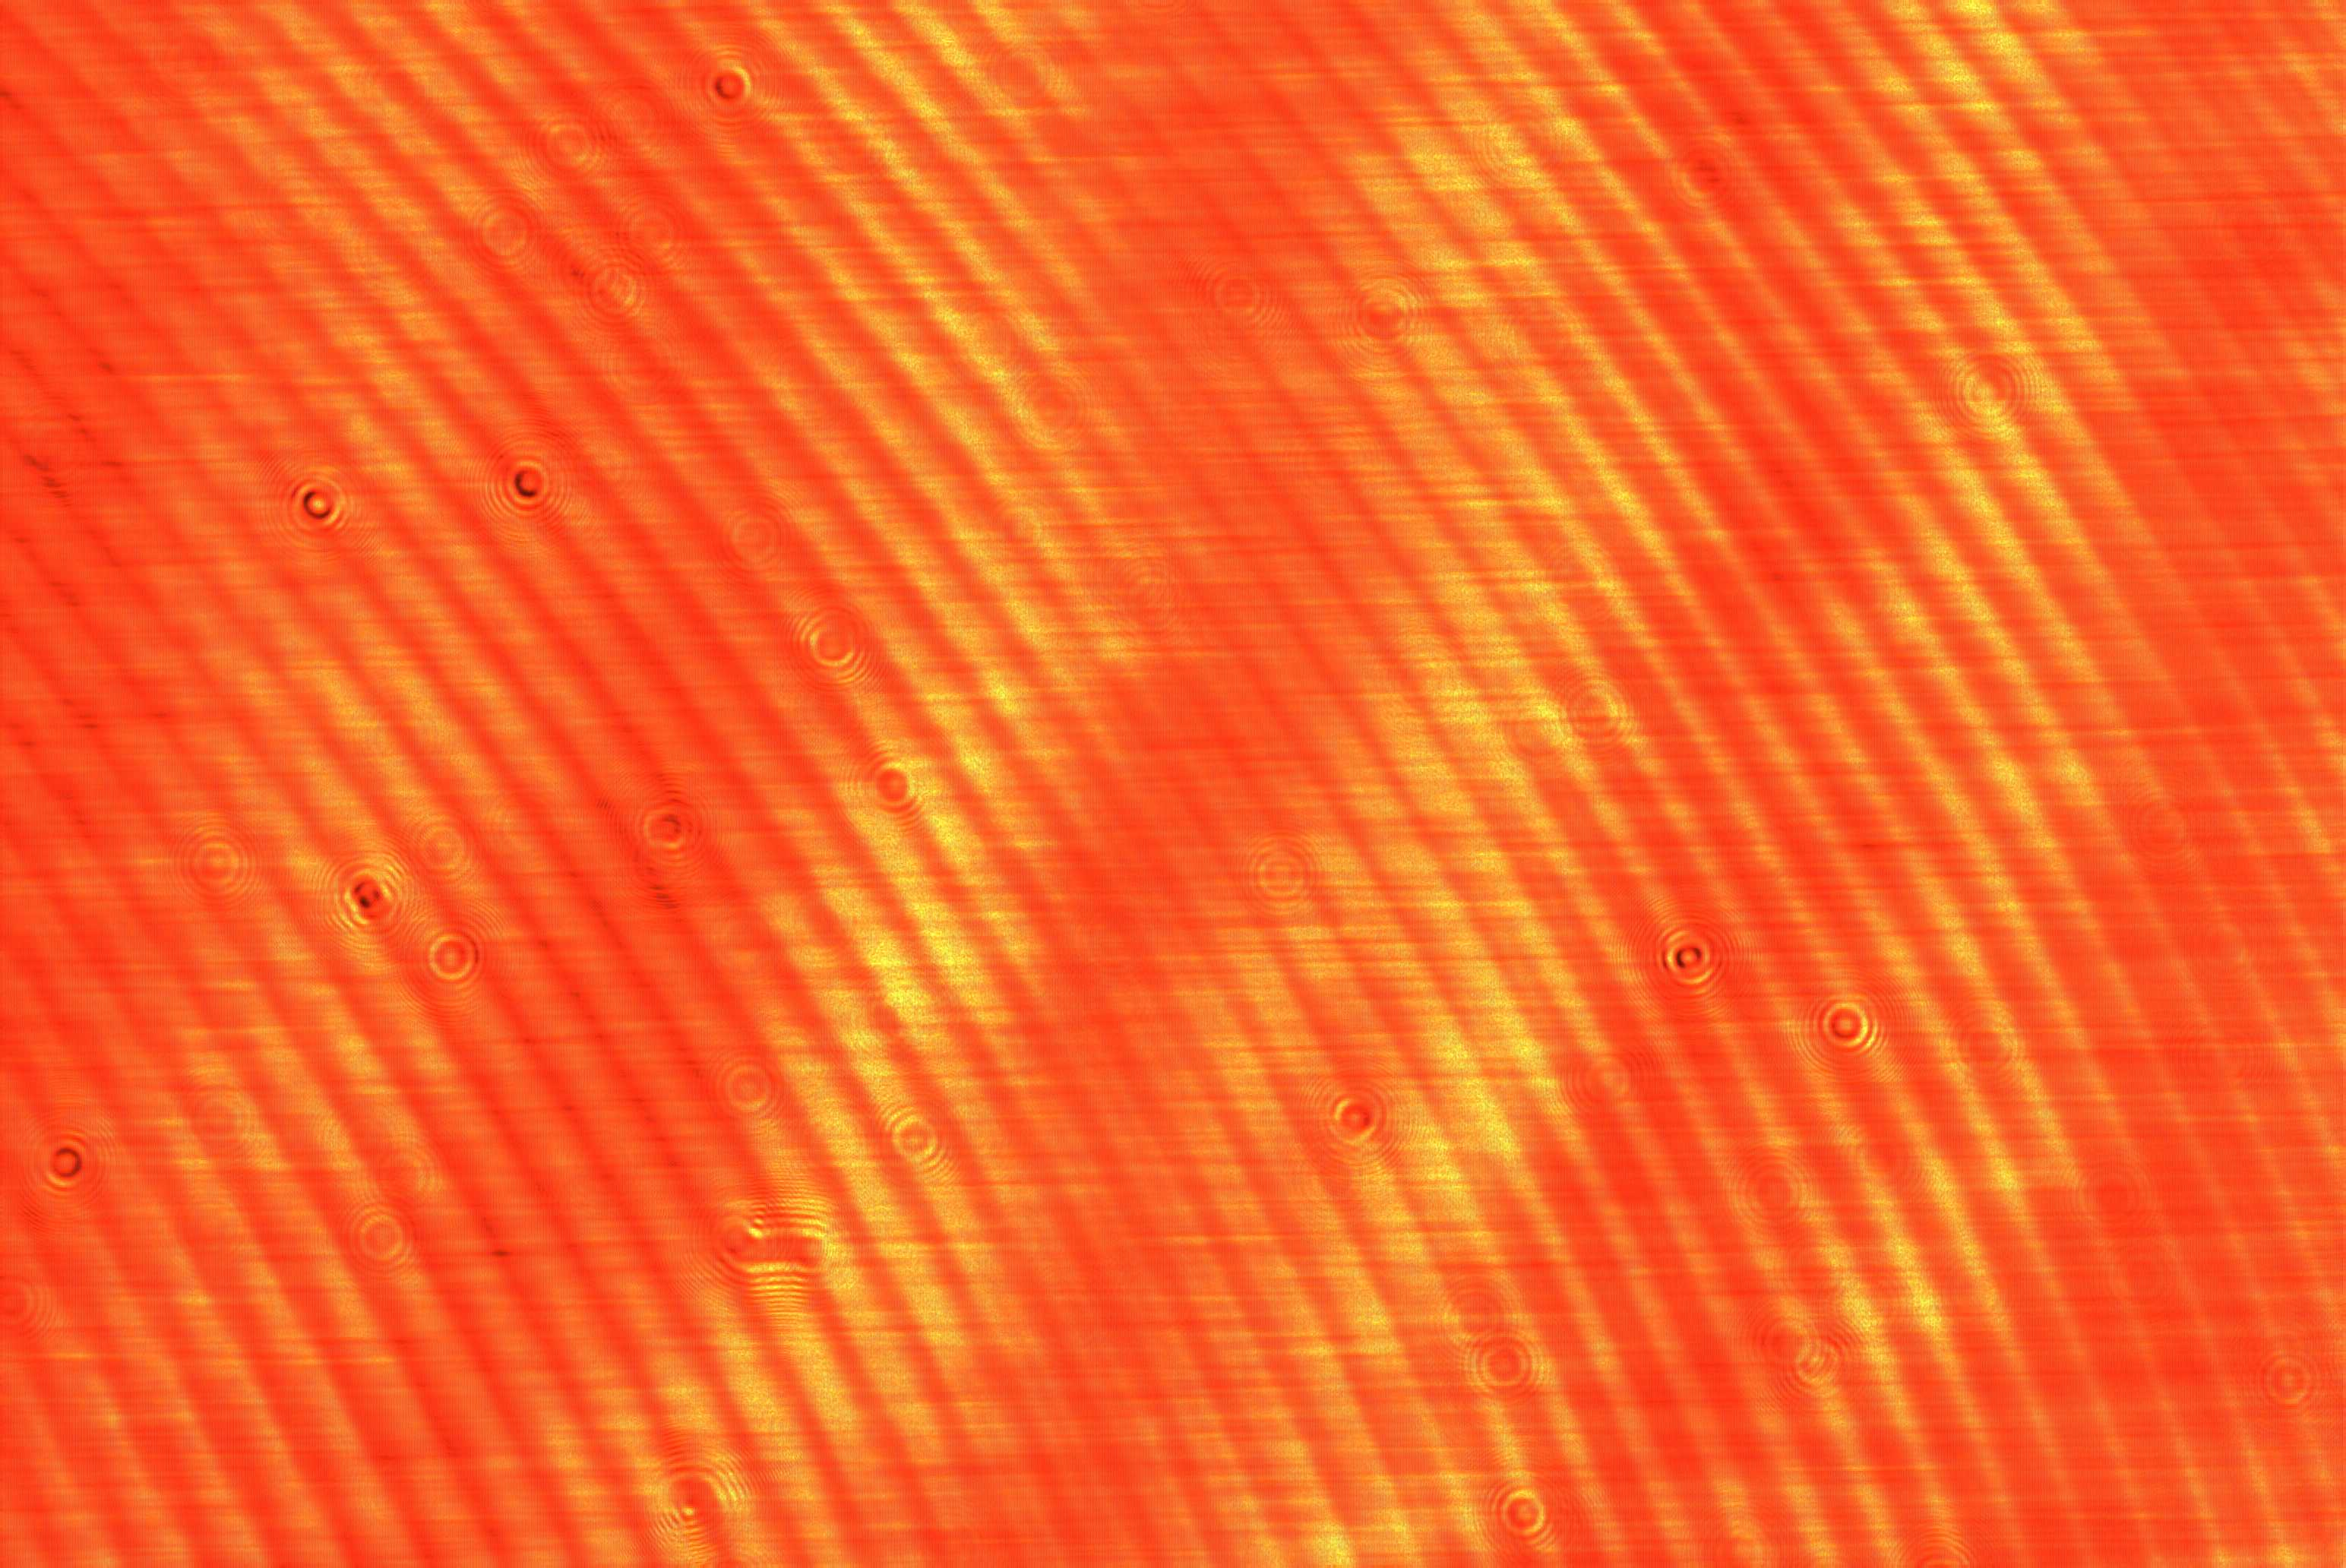
\includegraphics[width=0.3\textwidth]{attachments/fig.3.1.2.1.jpg}
			}
			\subfloat[0, 1 order]{\label{fig.3.1.2.2}
			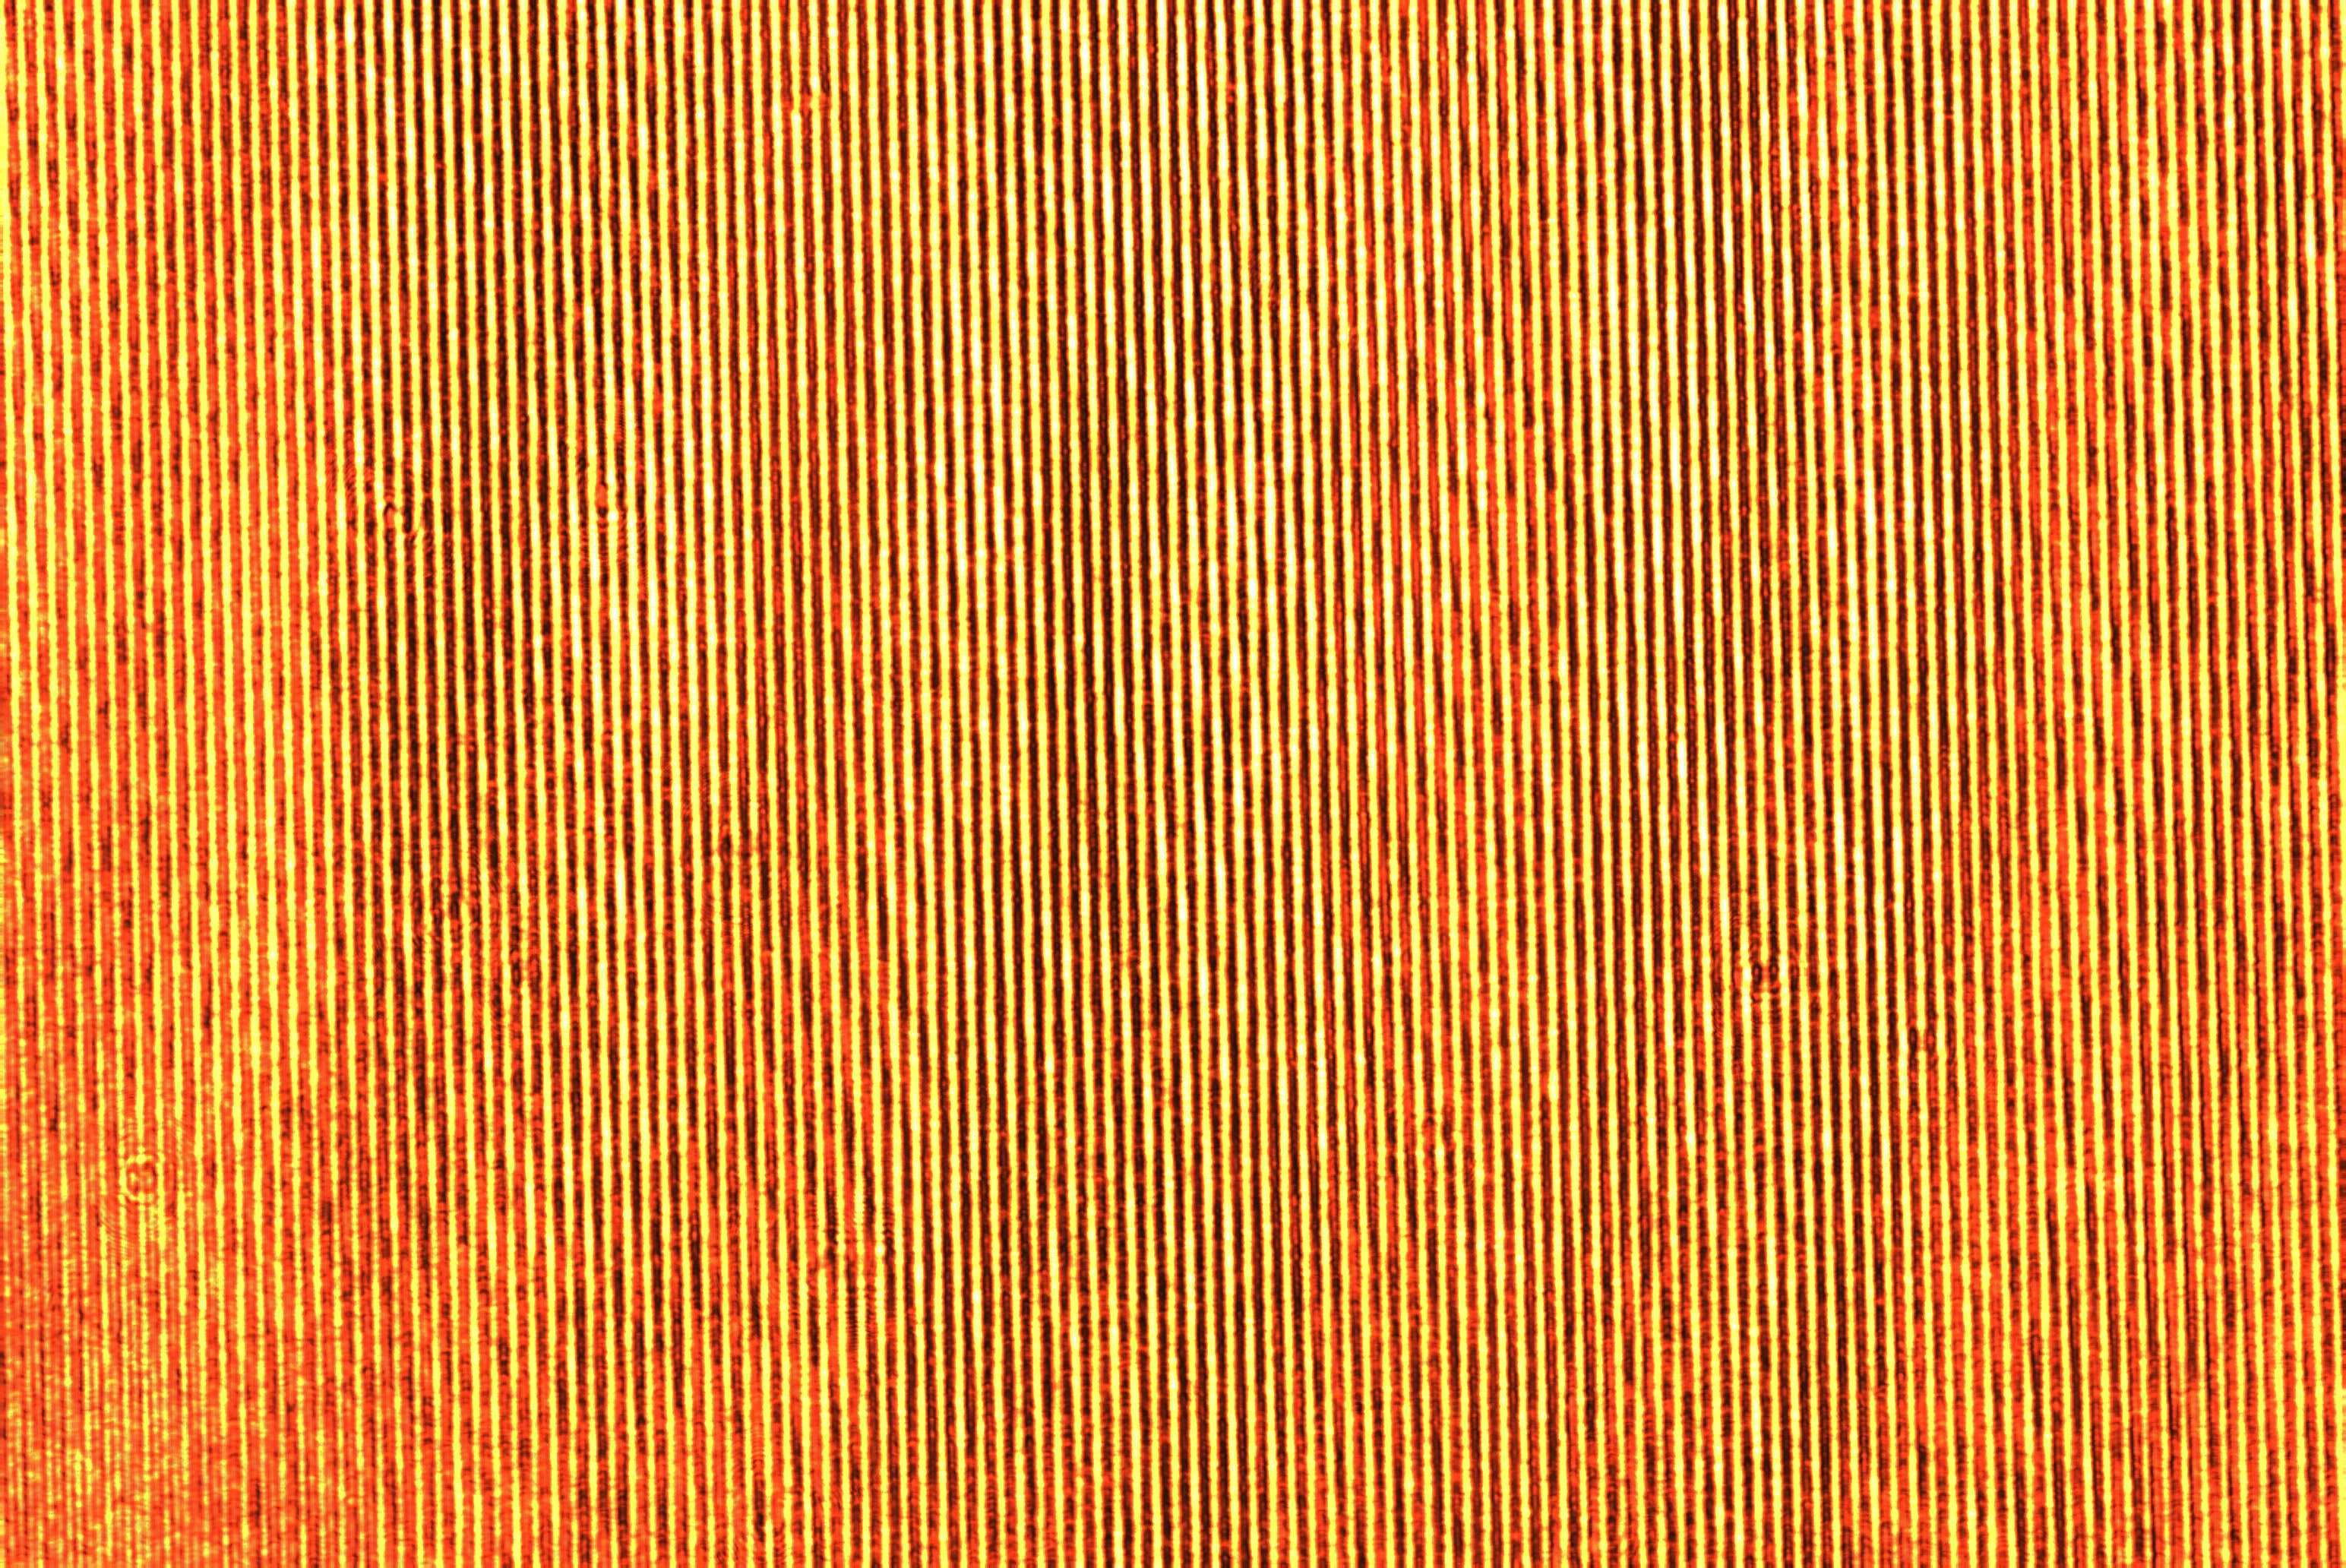
\includegraphics[width=0.3\textwidth]{attachments/fig.3.1.2.2.jpg}
			}
			\subfloat[0, 1, 2 order]{\label{fig.3.1.2.3}
			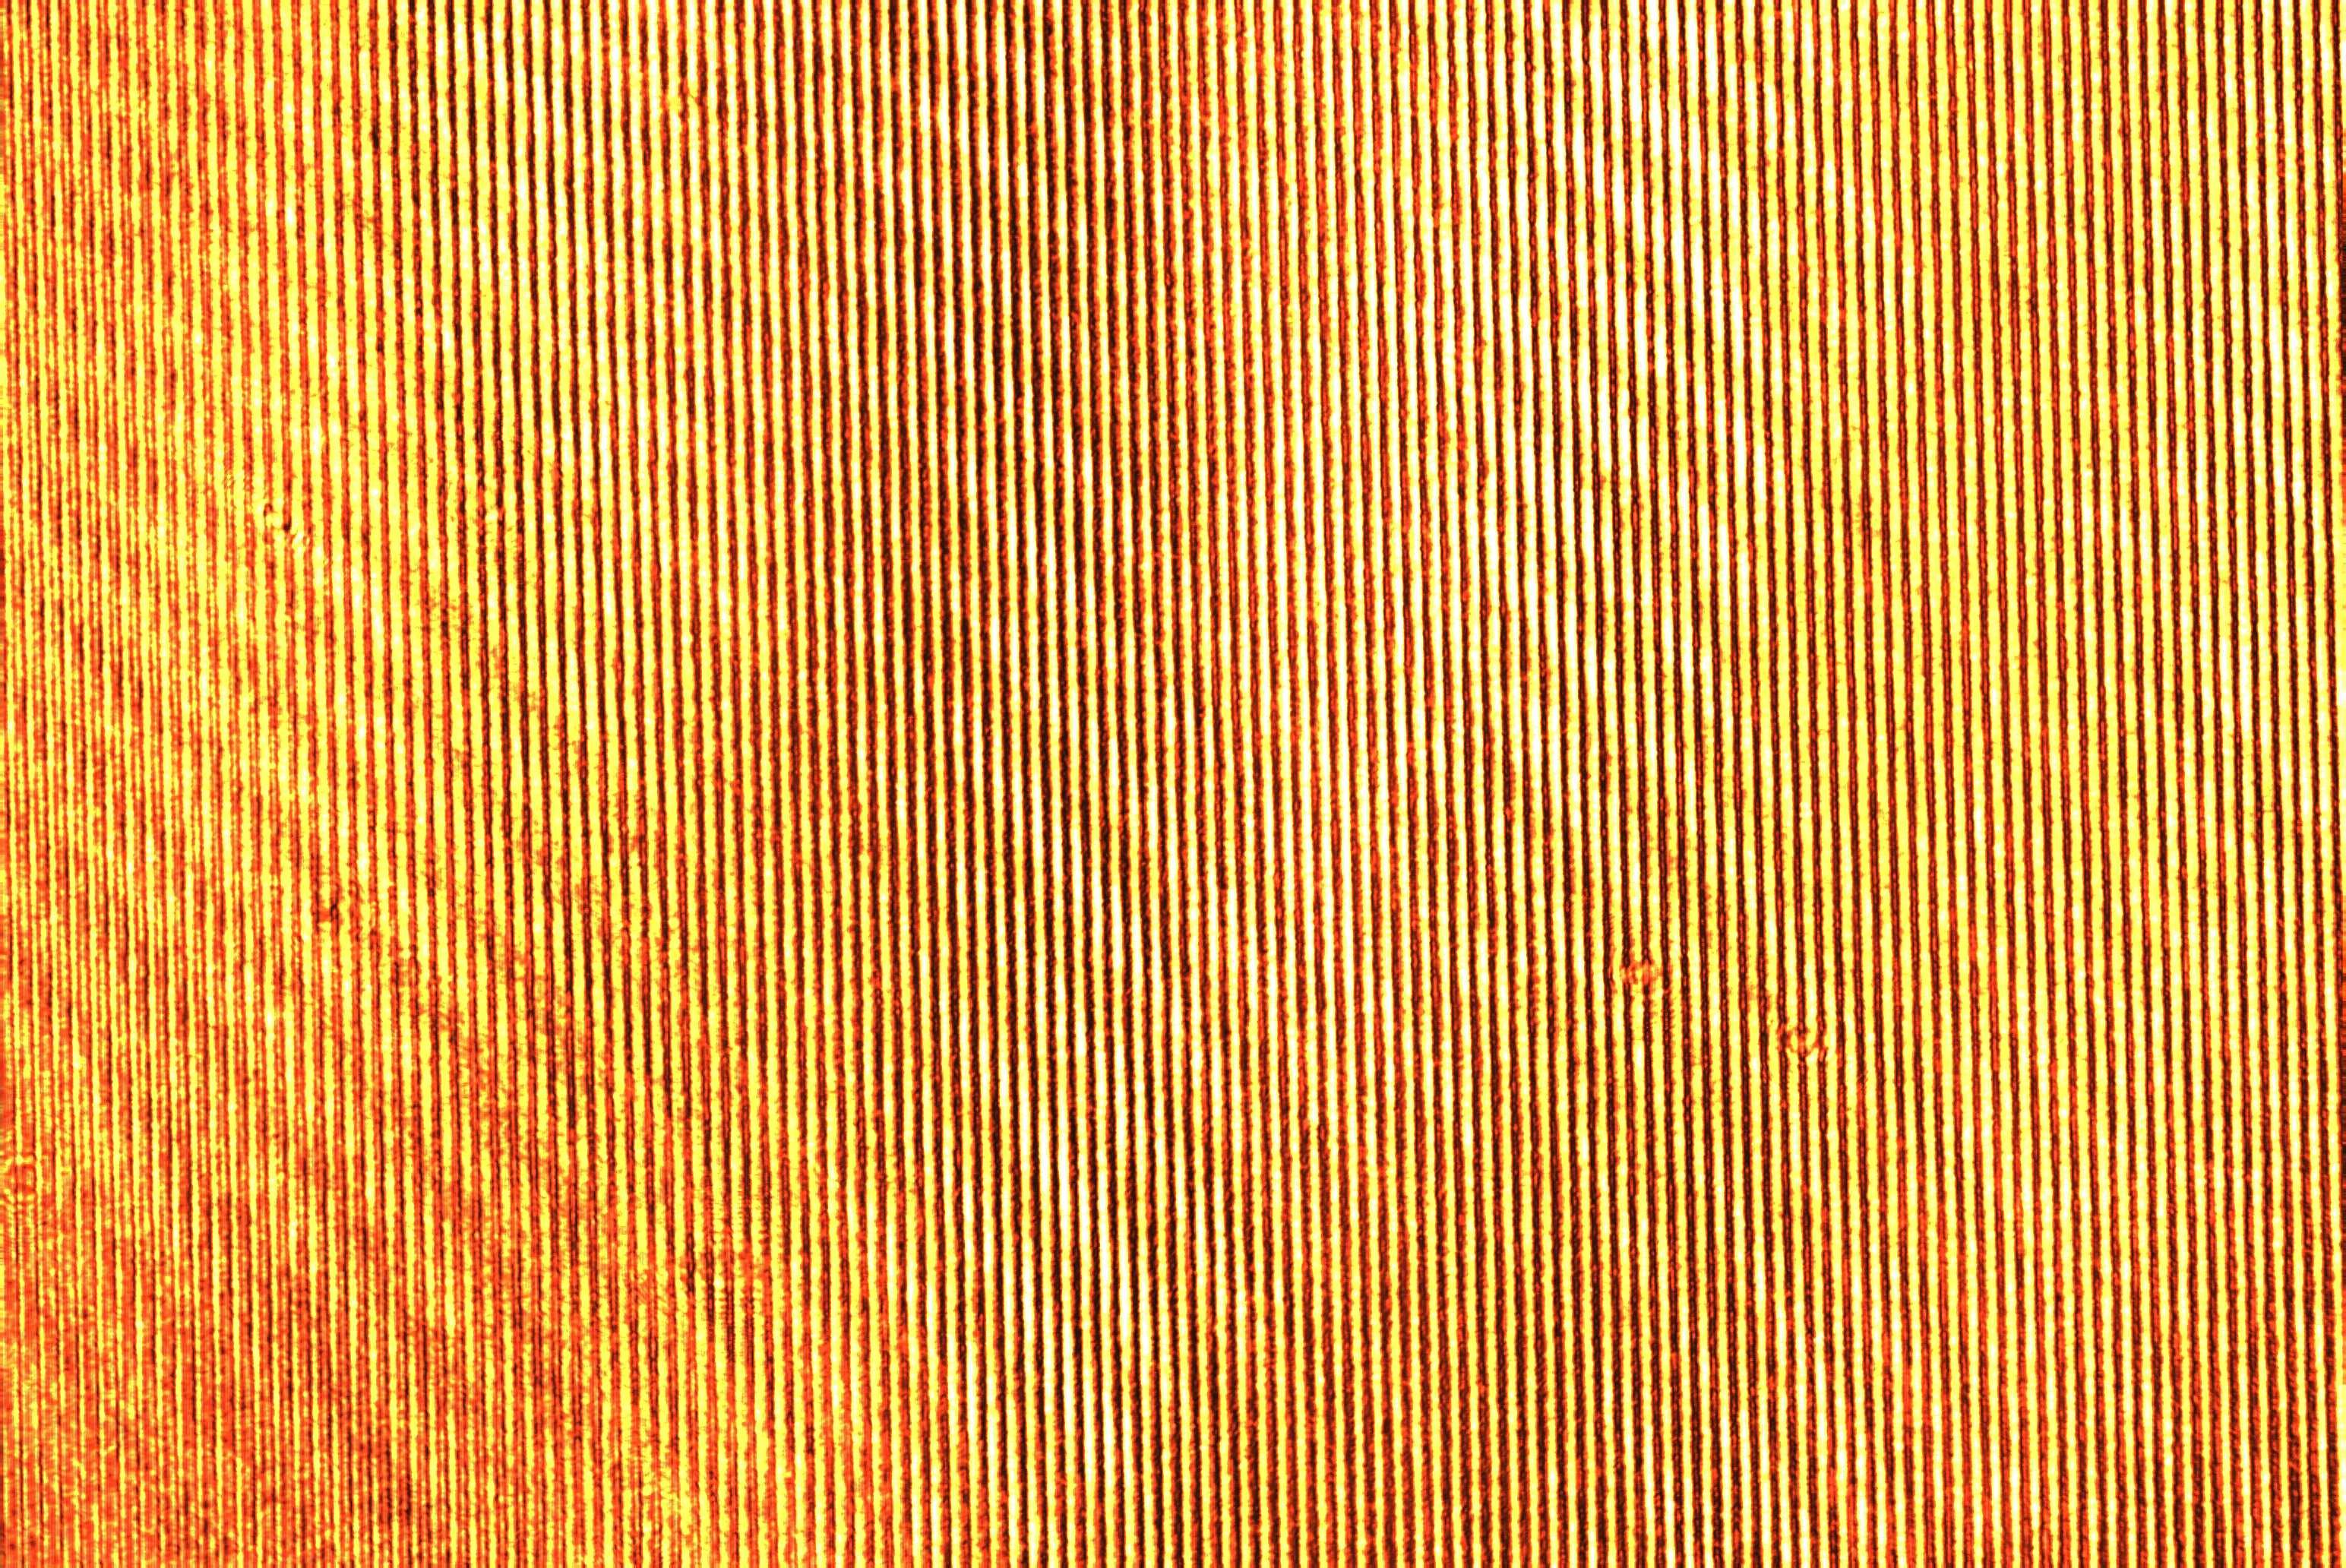
\includegraphics[width=0.3\textwidth]{attachments/fig.3.1.2.3.jpg}
			}
			\caption{\textbf{Diffraction experiments on 4f system}}
		\end{figure*}

		\begin{figure*}[htbp]
			\centering
			\subfloat[128T grating image]{\label{fig.3.2.0}
			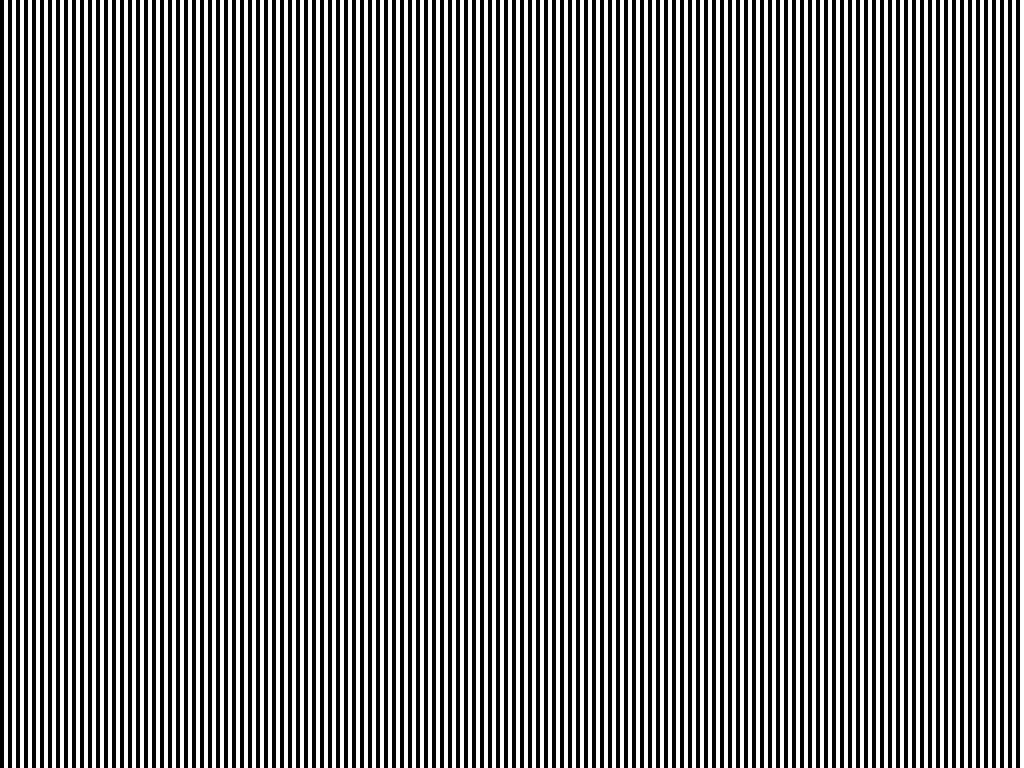
\includegraphics[width=0.3\textwidth]{attachments/fig.3.2.0.jpg}
			}		
			\subfloat[The spatial spectrum]{\label{fig.3.2.1.1}
			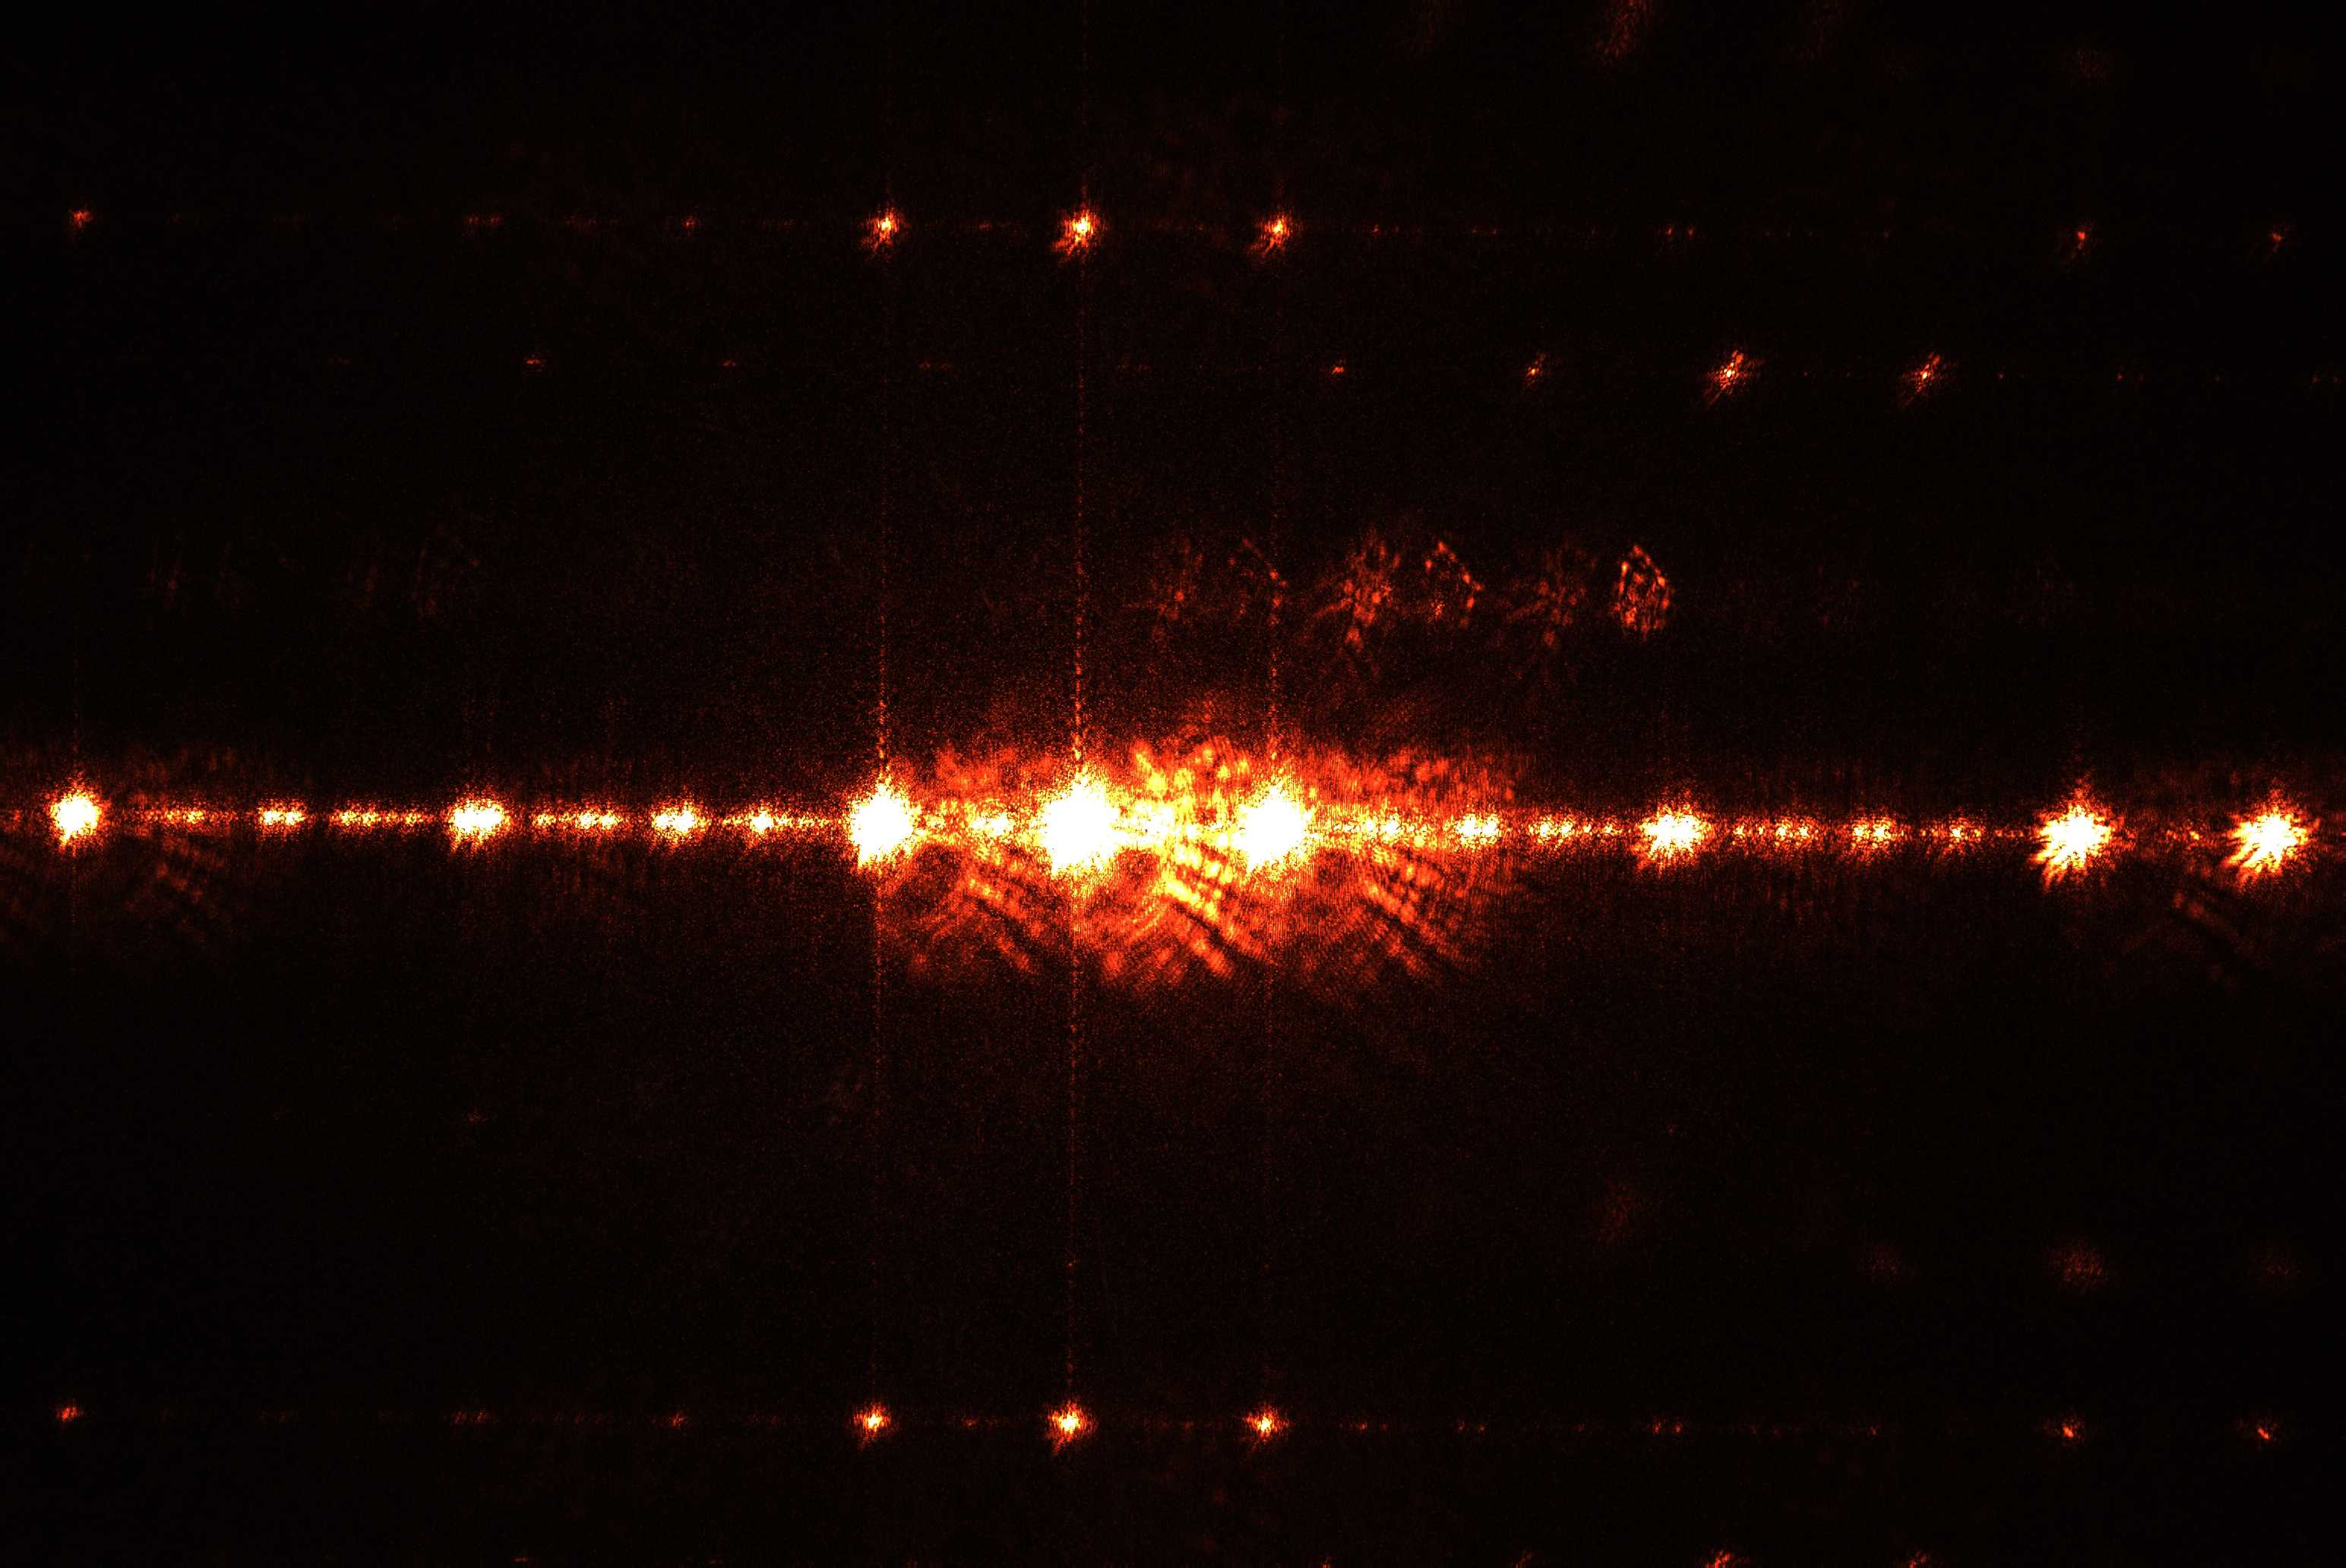
\includegraphics[width=0.3\textwidth]{attachments/fig.3.2.1.1.jpg}
			}
			\subfloat[The diffraction fringes]{\label{fig.3.2.1.2}
			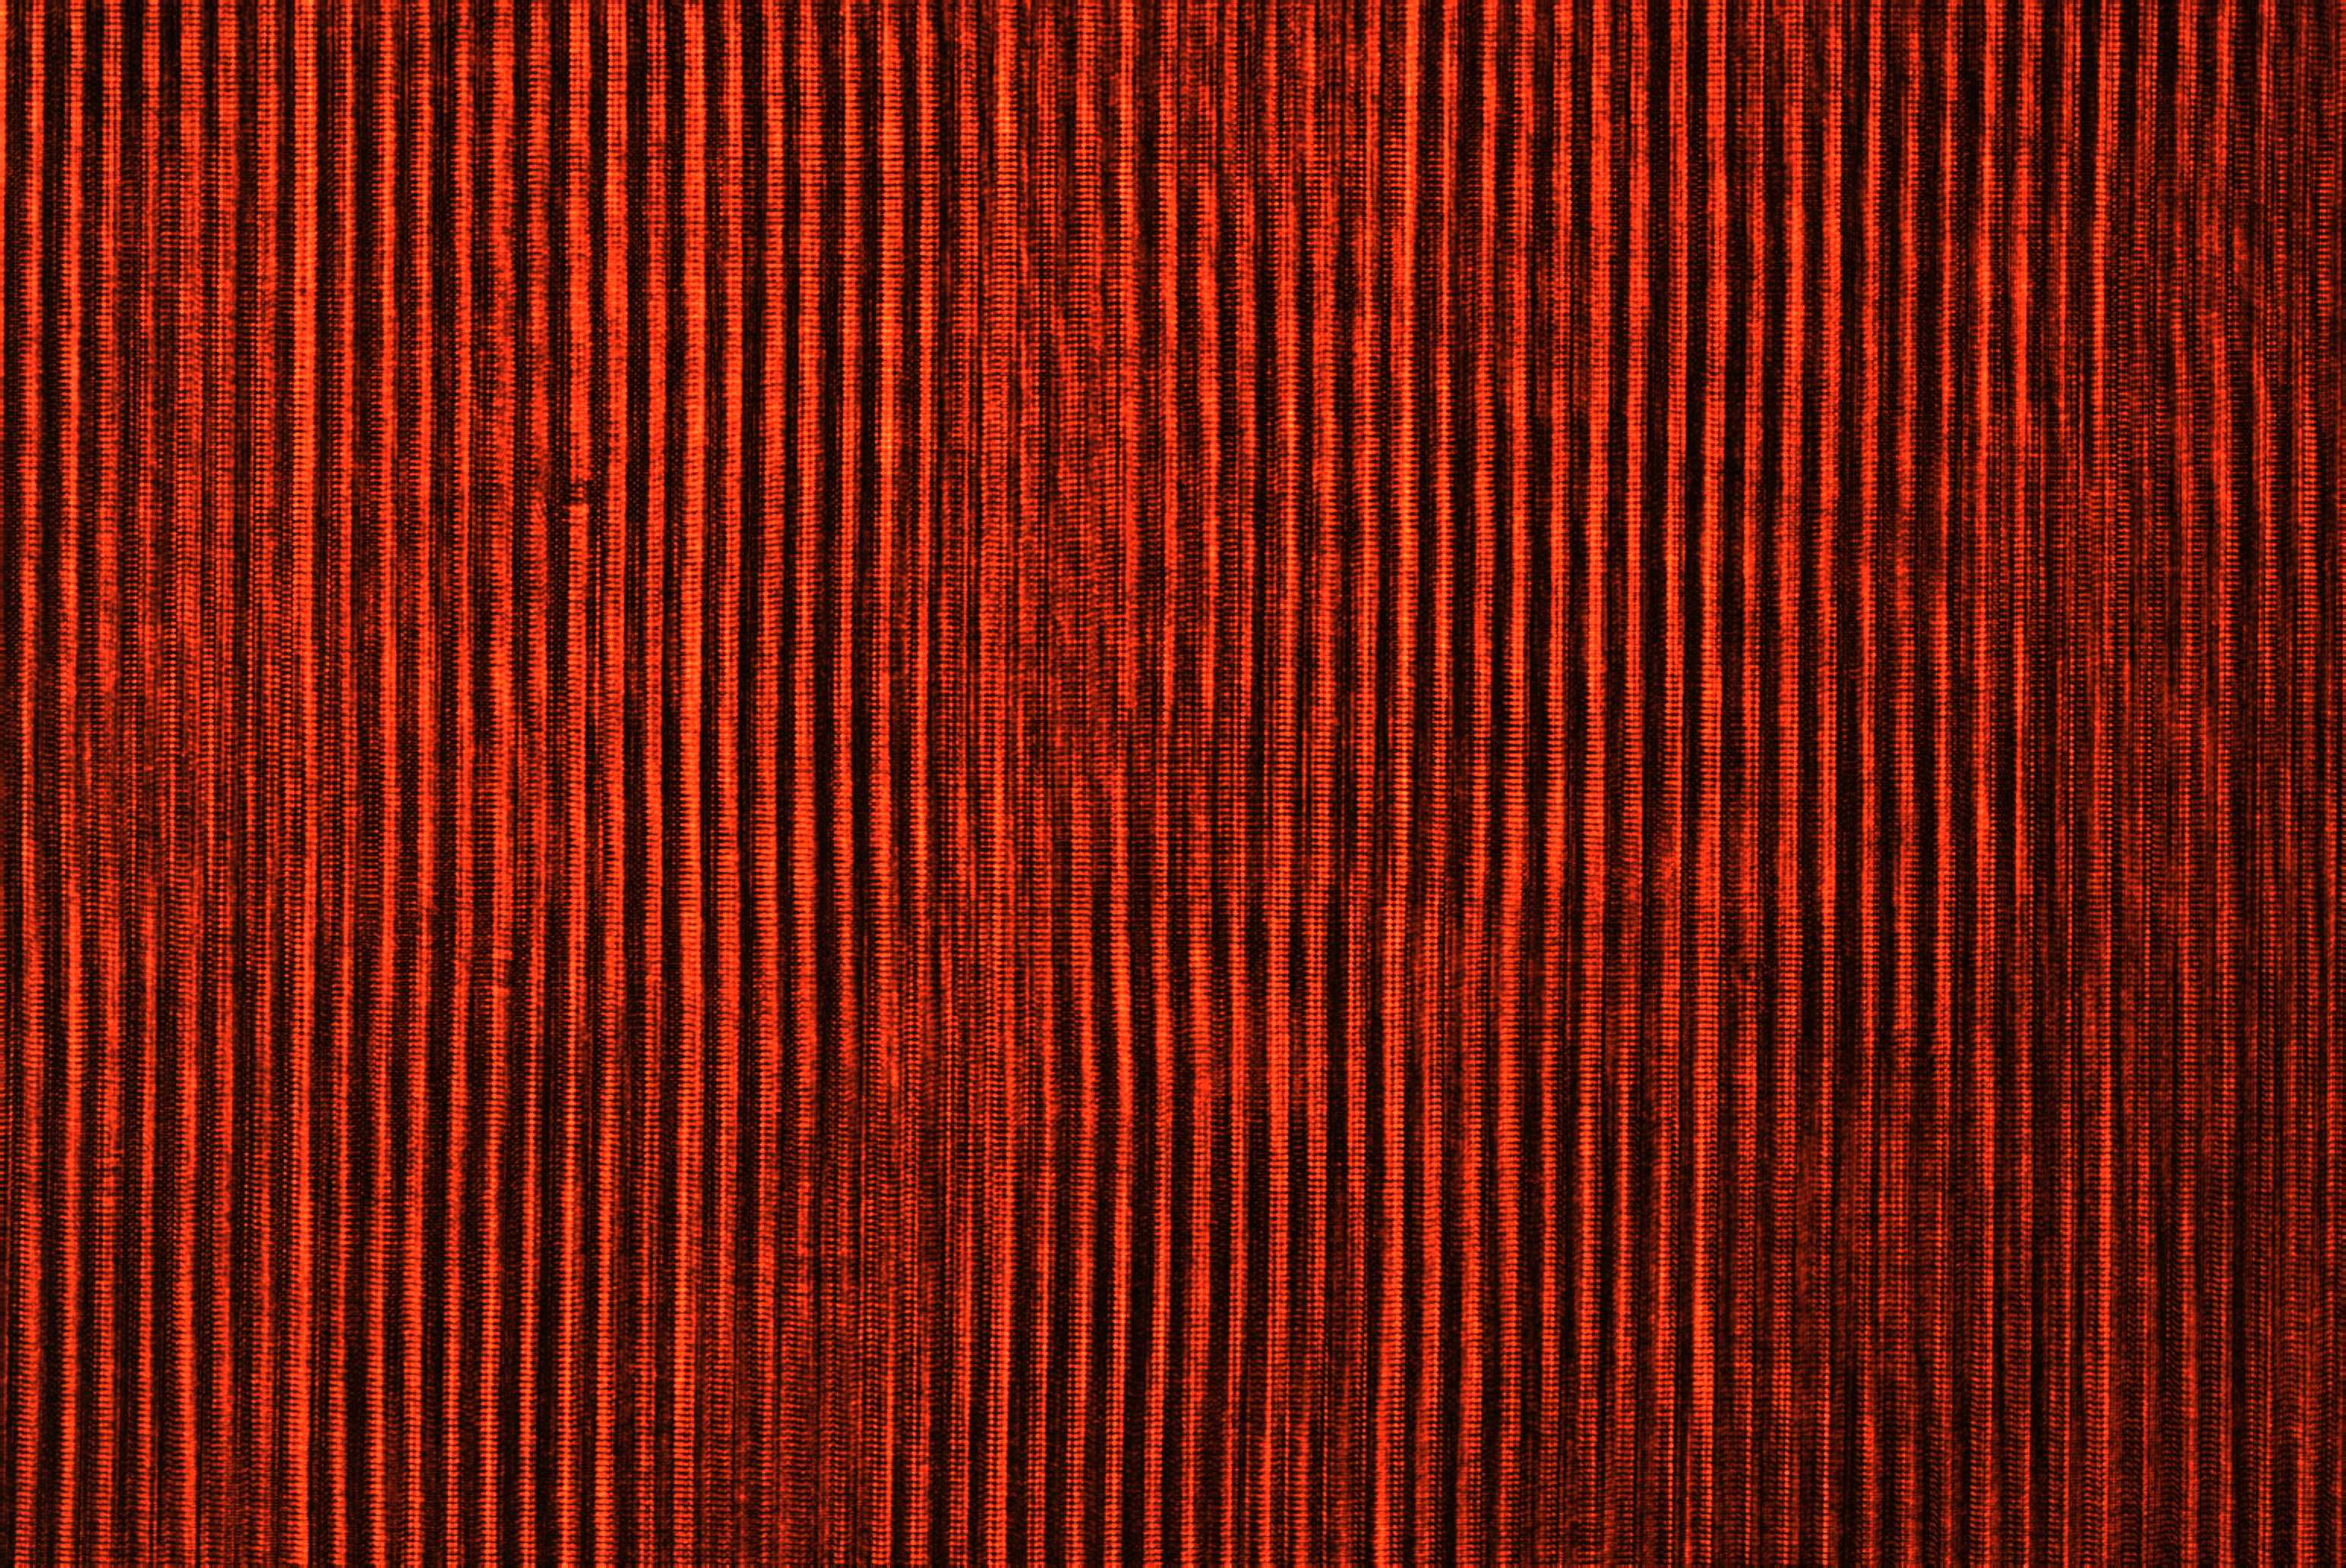
\includegraphics[width=0.3\textwidth]{attachments/fig.3.2.1.2.jpg}
			}

			\subfloat[0 order]{\label{fig.3.2.2.1}
			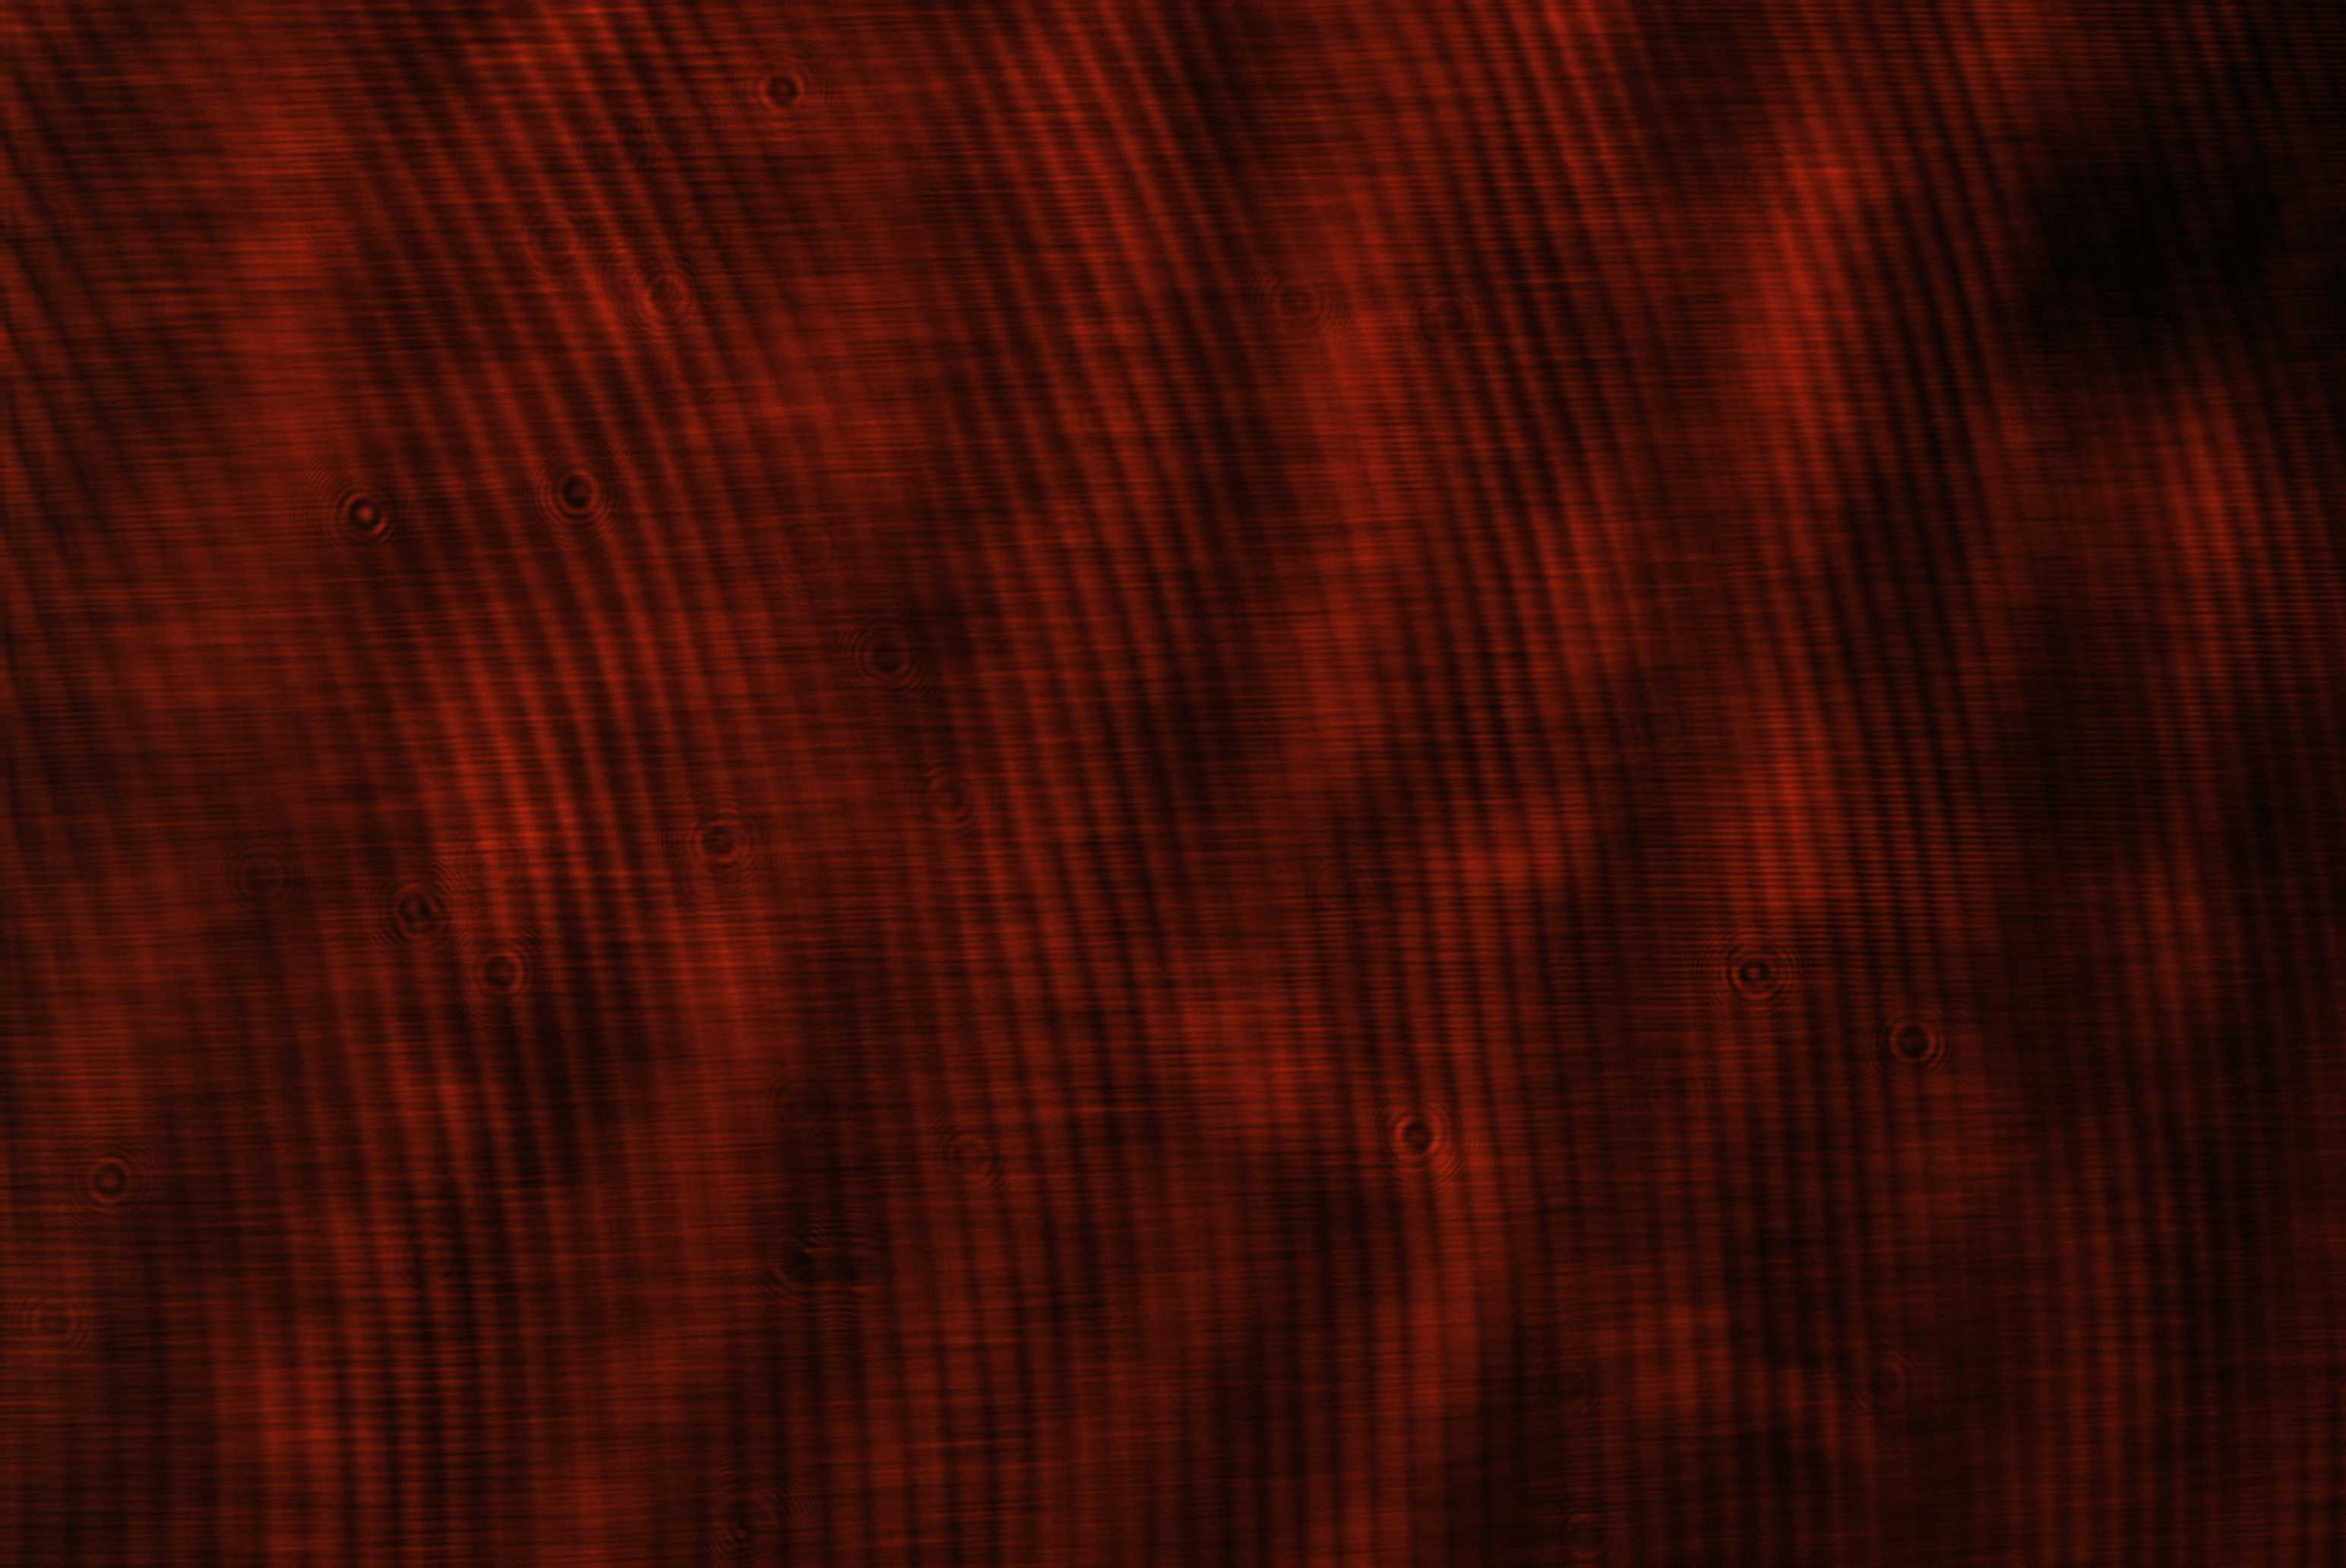
\includegraphics[width=0.3\textwidth]{attachments/fig.3.2.2.1.jpg}
			}
			\subfloat[0, 1 order]{\label{fig.3.2.2.2}
			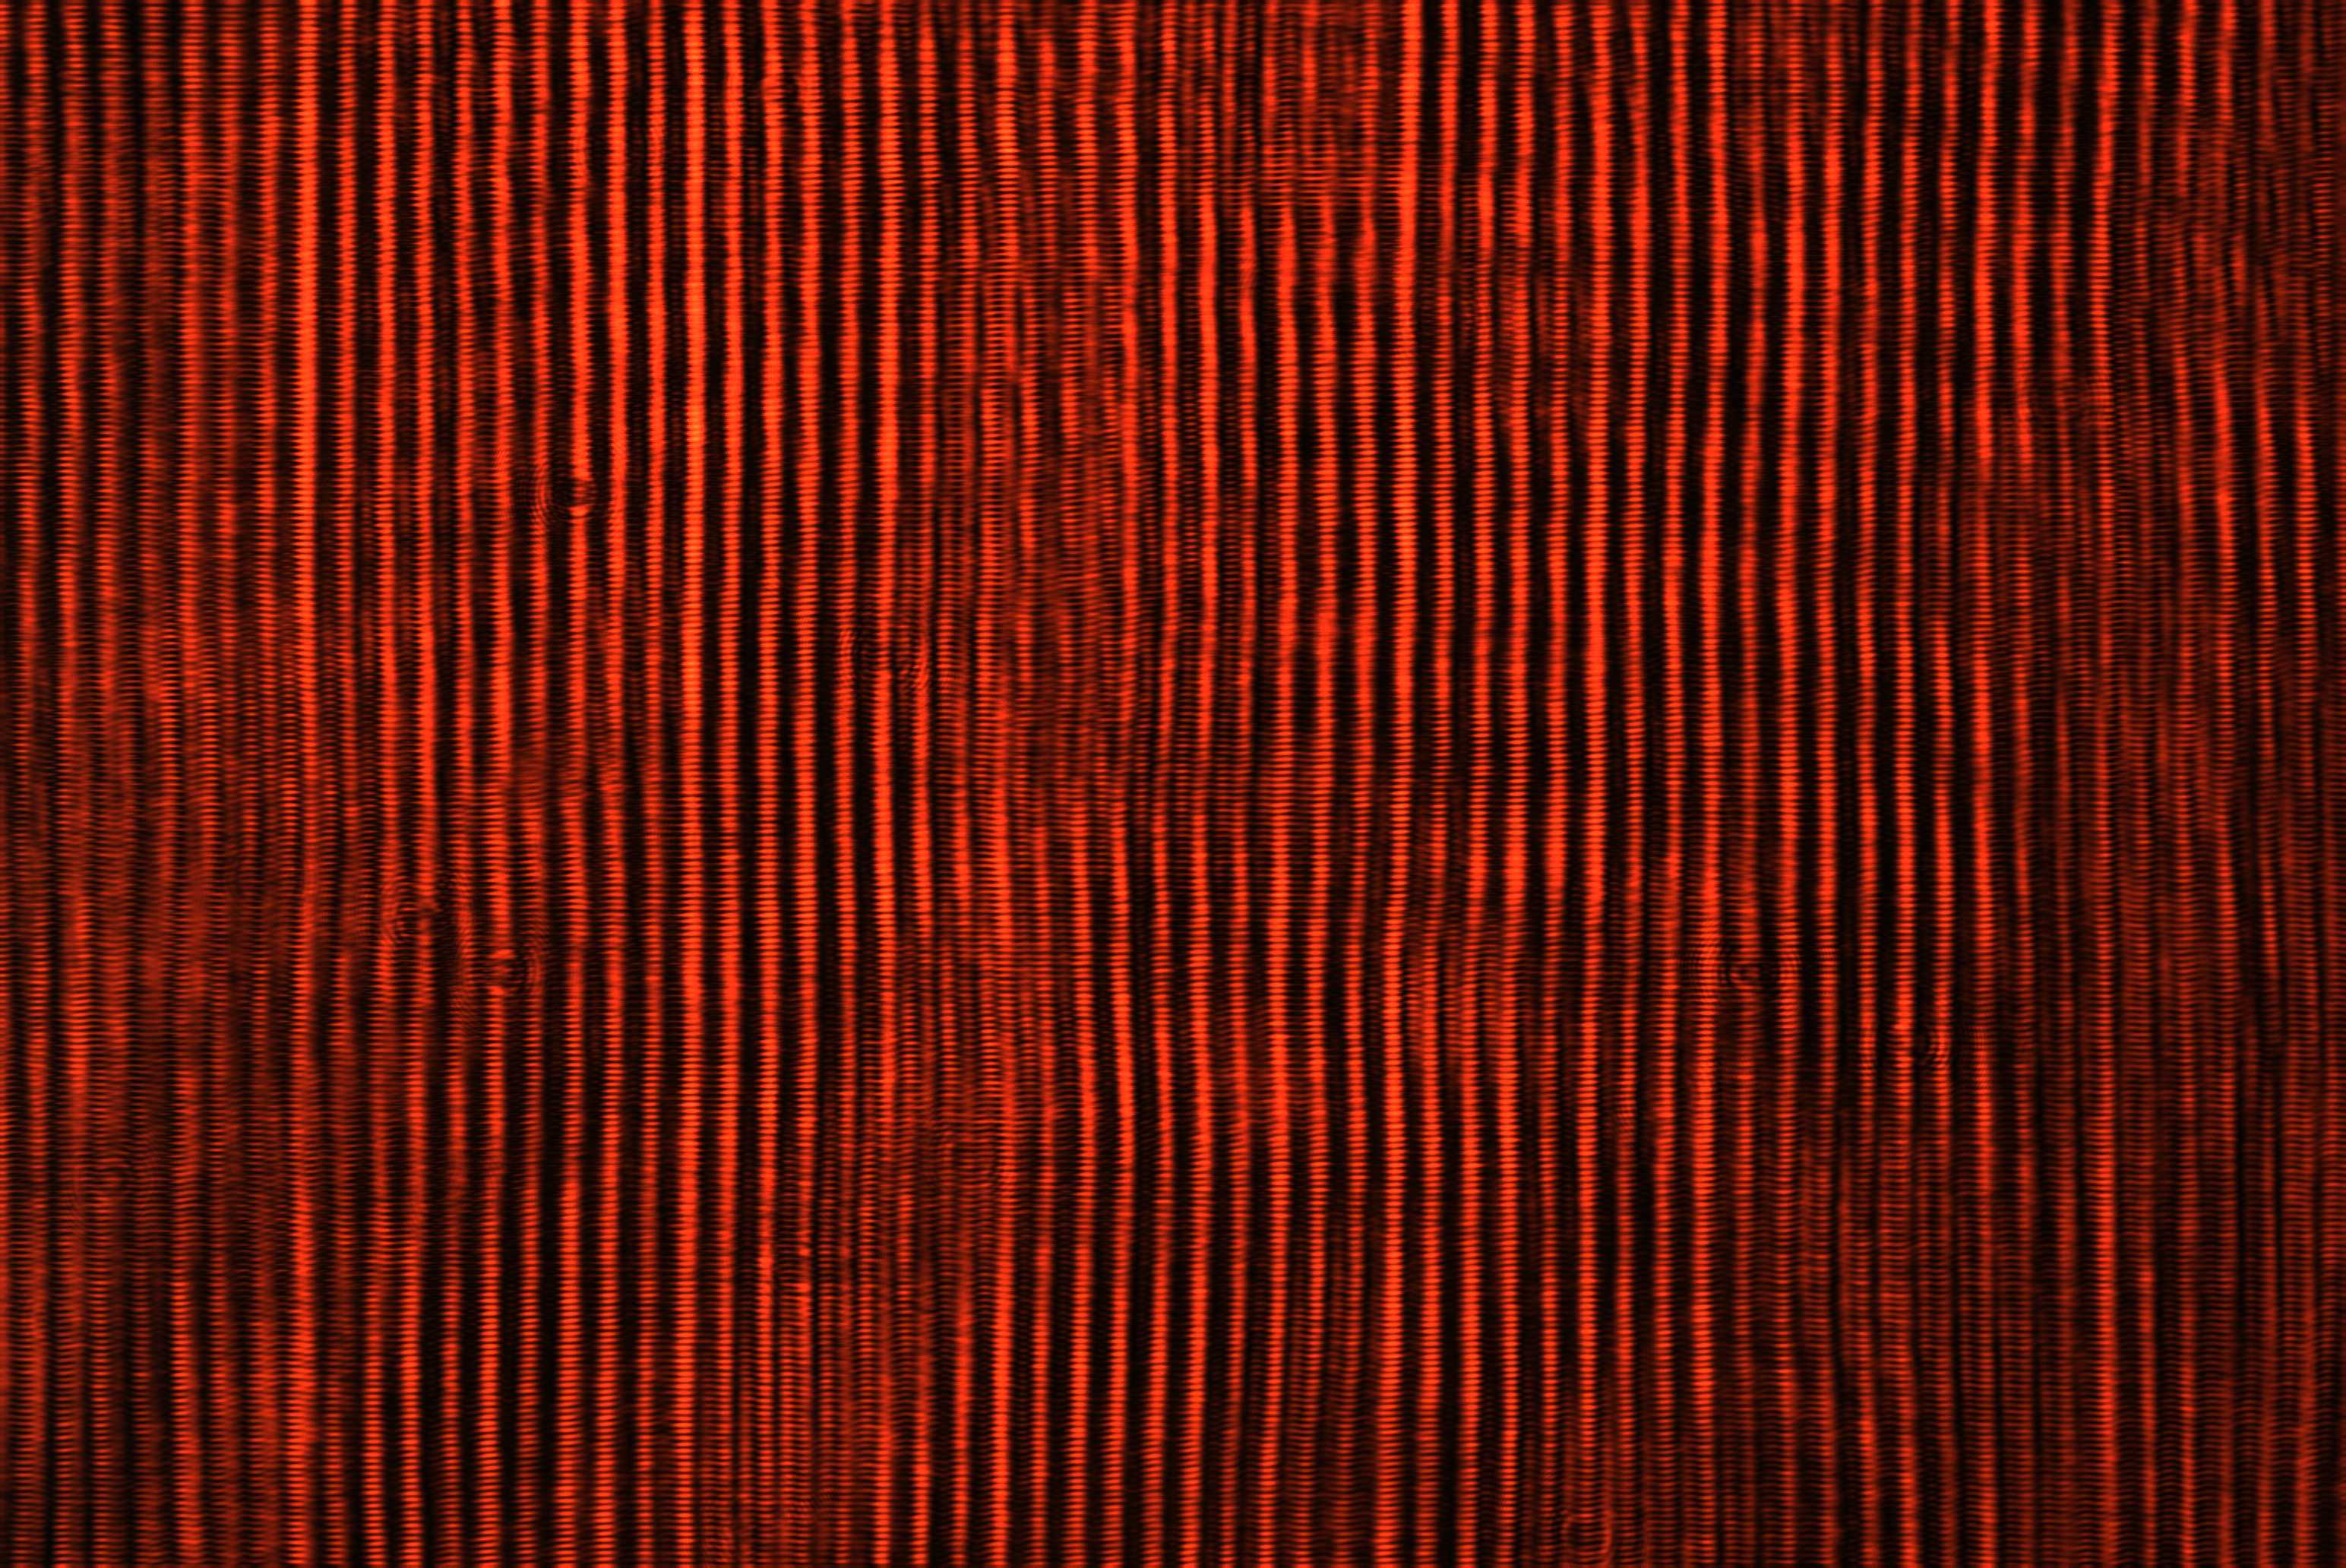
\includegraphics[width=0.3\textwidth]{attachments/fig.3.2.2.2.jpg}
			}
			\subfloat[circular aperture]{\label{fig.3.2.2.3}
			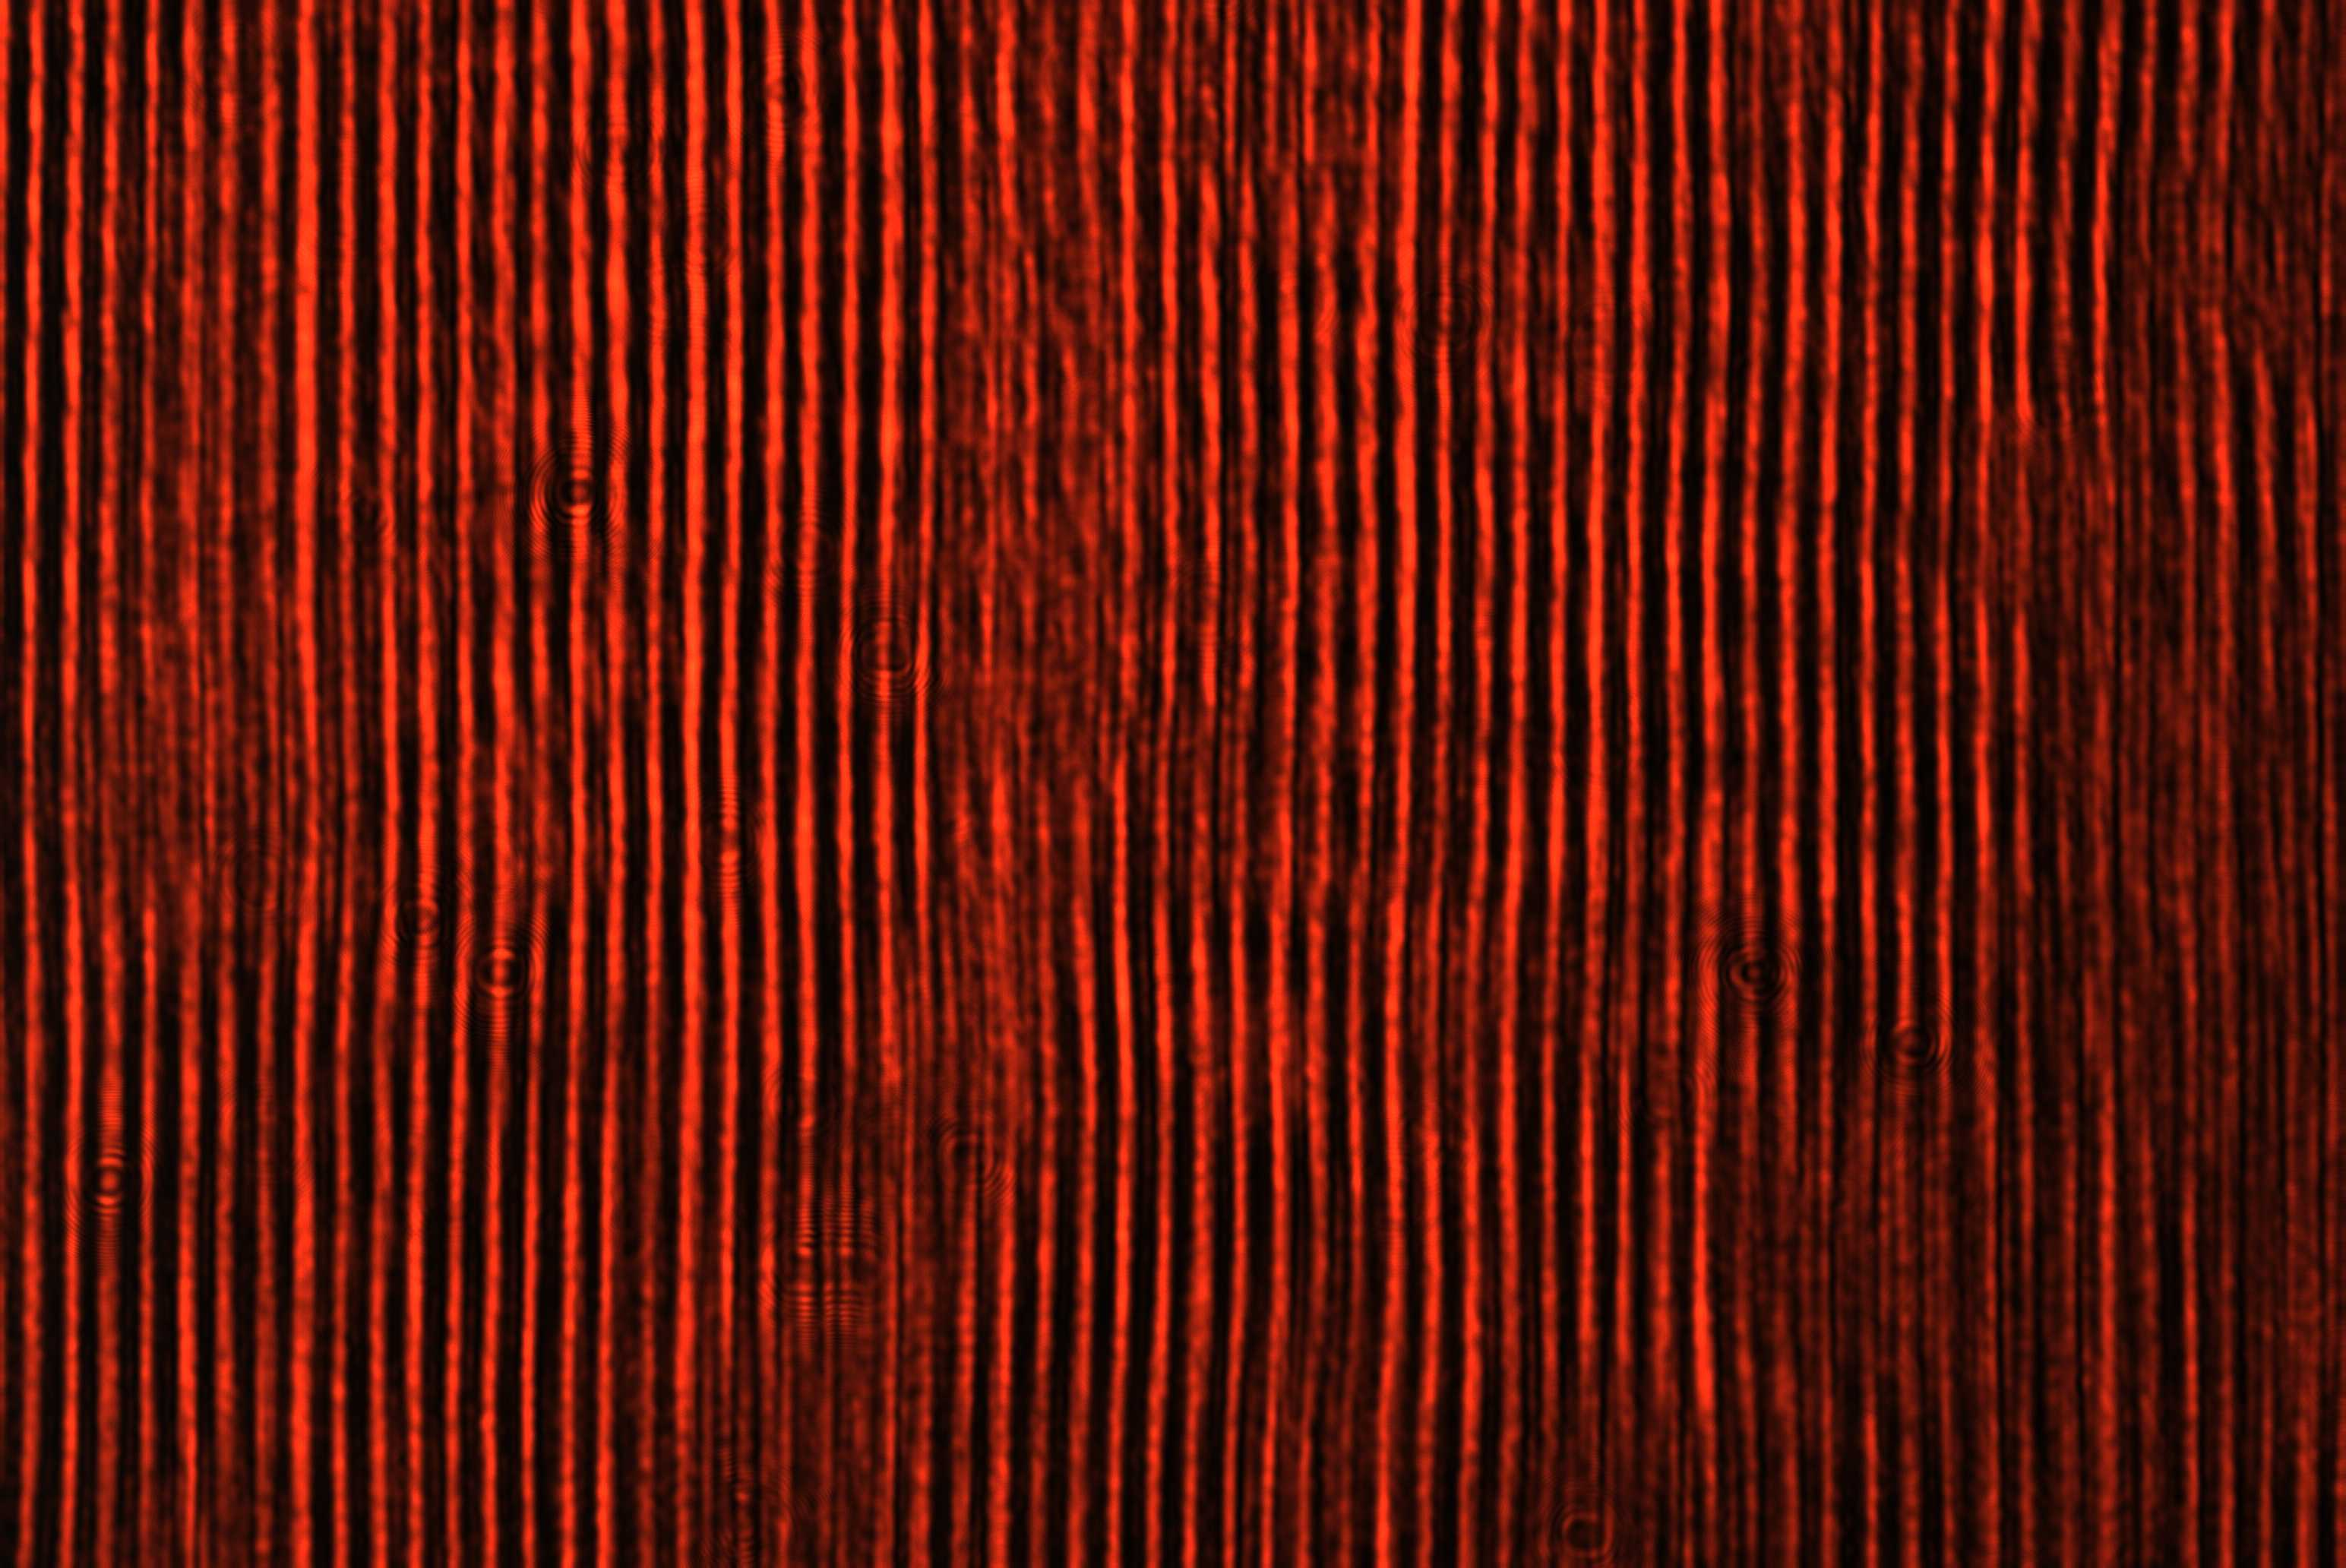
\includegraphics[width=0.3\textwidth]{attachments/fig.3.2.2.3.jpg}
			}
			\caption{\textbf{Diffraction experiments on single-lens system}}
		\end{figure*}

		We found that on $P_2$, both systems form a similar spatial spectrum, and on $P_3$, the diffraction patterns of the two systems are similar.
		If only 0 order spot was allowed to pass, there were no diffraction fringes on $P_3$; if 1 order spots were also allowed, the fringes appear, but still dimmer than the diffraction patterns with no aperture. 
		These phenomena verify Abbe's theory, which states that the image is formed by diffraction of beams from $P_2$. 
		If only the 0 order spot is allowed to pass, no diffraction will happen, i.e. there will be no diffraction patterns.
		If more spots are allowed to pass, the diffraction patterns are clearer and brighter as more detail information carried by spots of higher orders are added.
		
		Although the results of the two systems were generally similar, there were still some differences.
		One difference we observed is that there were spots distributed in vertical ornamentation on the spatial spectrum of the single-lens system comparing with the 4f system.
		We consider that this is caused by the rasterization effects of the SLM. As previously introduced, SLM is composed of various of pixels ordered in 2D microarray (Fig. \ref{fig.illus-1.1}).
		Between the adjacent pixels, there is a gap, which leads to the rasterization of the image and causes the additional diffraction in vertical orientation.
		This hypothesis is supported by the diffraction pattern when the circular aperture was applied, which was dimmer because of loss of information carried by the spots in vertical orientation.

		Comparing the two systems, although there are some slight differences, generally the results are similar, which verifies the effectiveness of the single-lens system and SLM in optical information processing.

		\subsubsection{Spatial filtering}
		Basing on the Abbe's theory of image formation, we conducted the high-pass (Fig. \ref{fig.3.3.1.3}), low-pass(Fig. \ref{fig.3.3.1.4}) and band-pass filtering in different orientations (Fig. \ref{fig.3.3.2}) to realize the optical information processing.
		
		Comparing the results of high-pass filtering and low-pass filtering with the original image, we found that after high-pass filtering, the edge of the image was sharpened and the definition was improved;
		while after low-pass filtering, the brightness was greatly reduced due to loss of the zero order spot, which normally contributes most of the energy, but the noise was also removed.
		
		The effects of band-pass filtering in different orientations are shown in Fig. \ref{fig.3.3.2} and summarized in Tab. \ref{tab.3.1}. 
		We found that as we rotated the band-pass filter, the orientation of the fringes rotated accordingly. 
		As we considered the fringe space, we found that the number of pixels per 10 fringes of the $0^{o}$ and $90^{o}$ orientations was approximately $\sqrt{2}$ times as the $45^{o}$ and $135^{o}$ orientations.
		According to multislit diffraction theory, the fringe space is inversely proportional to the grating constant. As the filter rotated $45^o$, the grating constant increased $\sqrt{2}$ times, which could explain our results. 

		These results show the application of spatial filtering in optical information processing.


		\begin{figure*}[htbp]
			\centering
			\subfloat[Object]{\label{fig.3.3.1.1}
			
\includegraphics[width=0.3\textwidth]{attachments/fig.3.3.1.1.jpg}
			}
			\subfloat[Image]{\label{fig.3.3.1.2}
			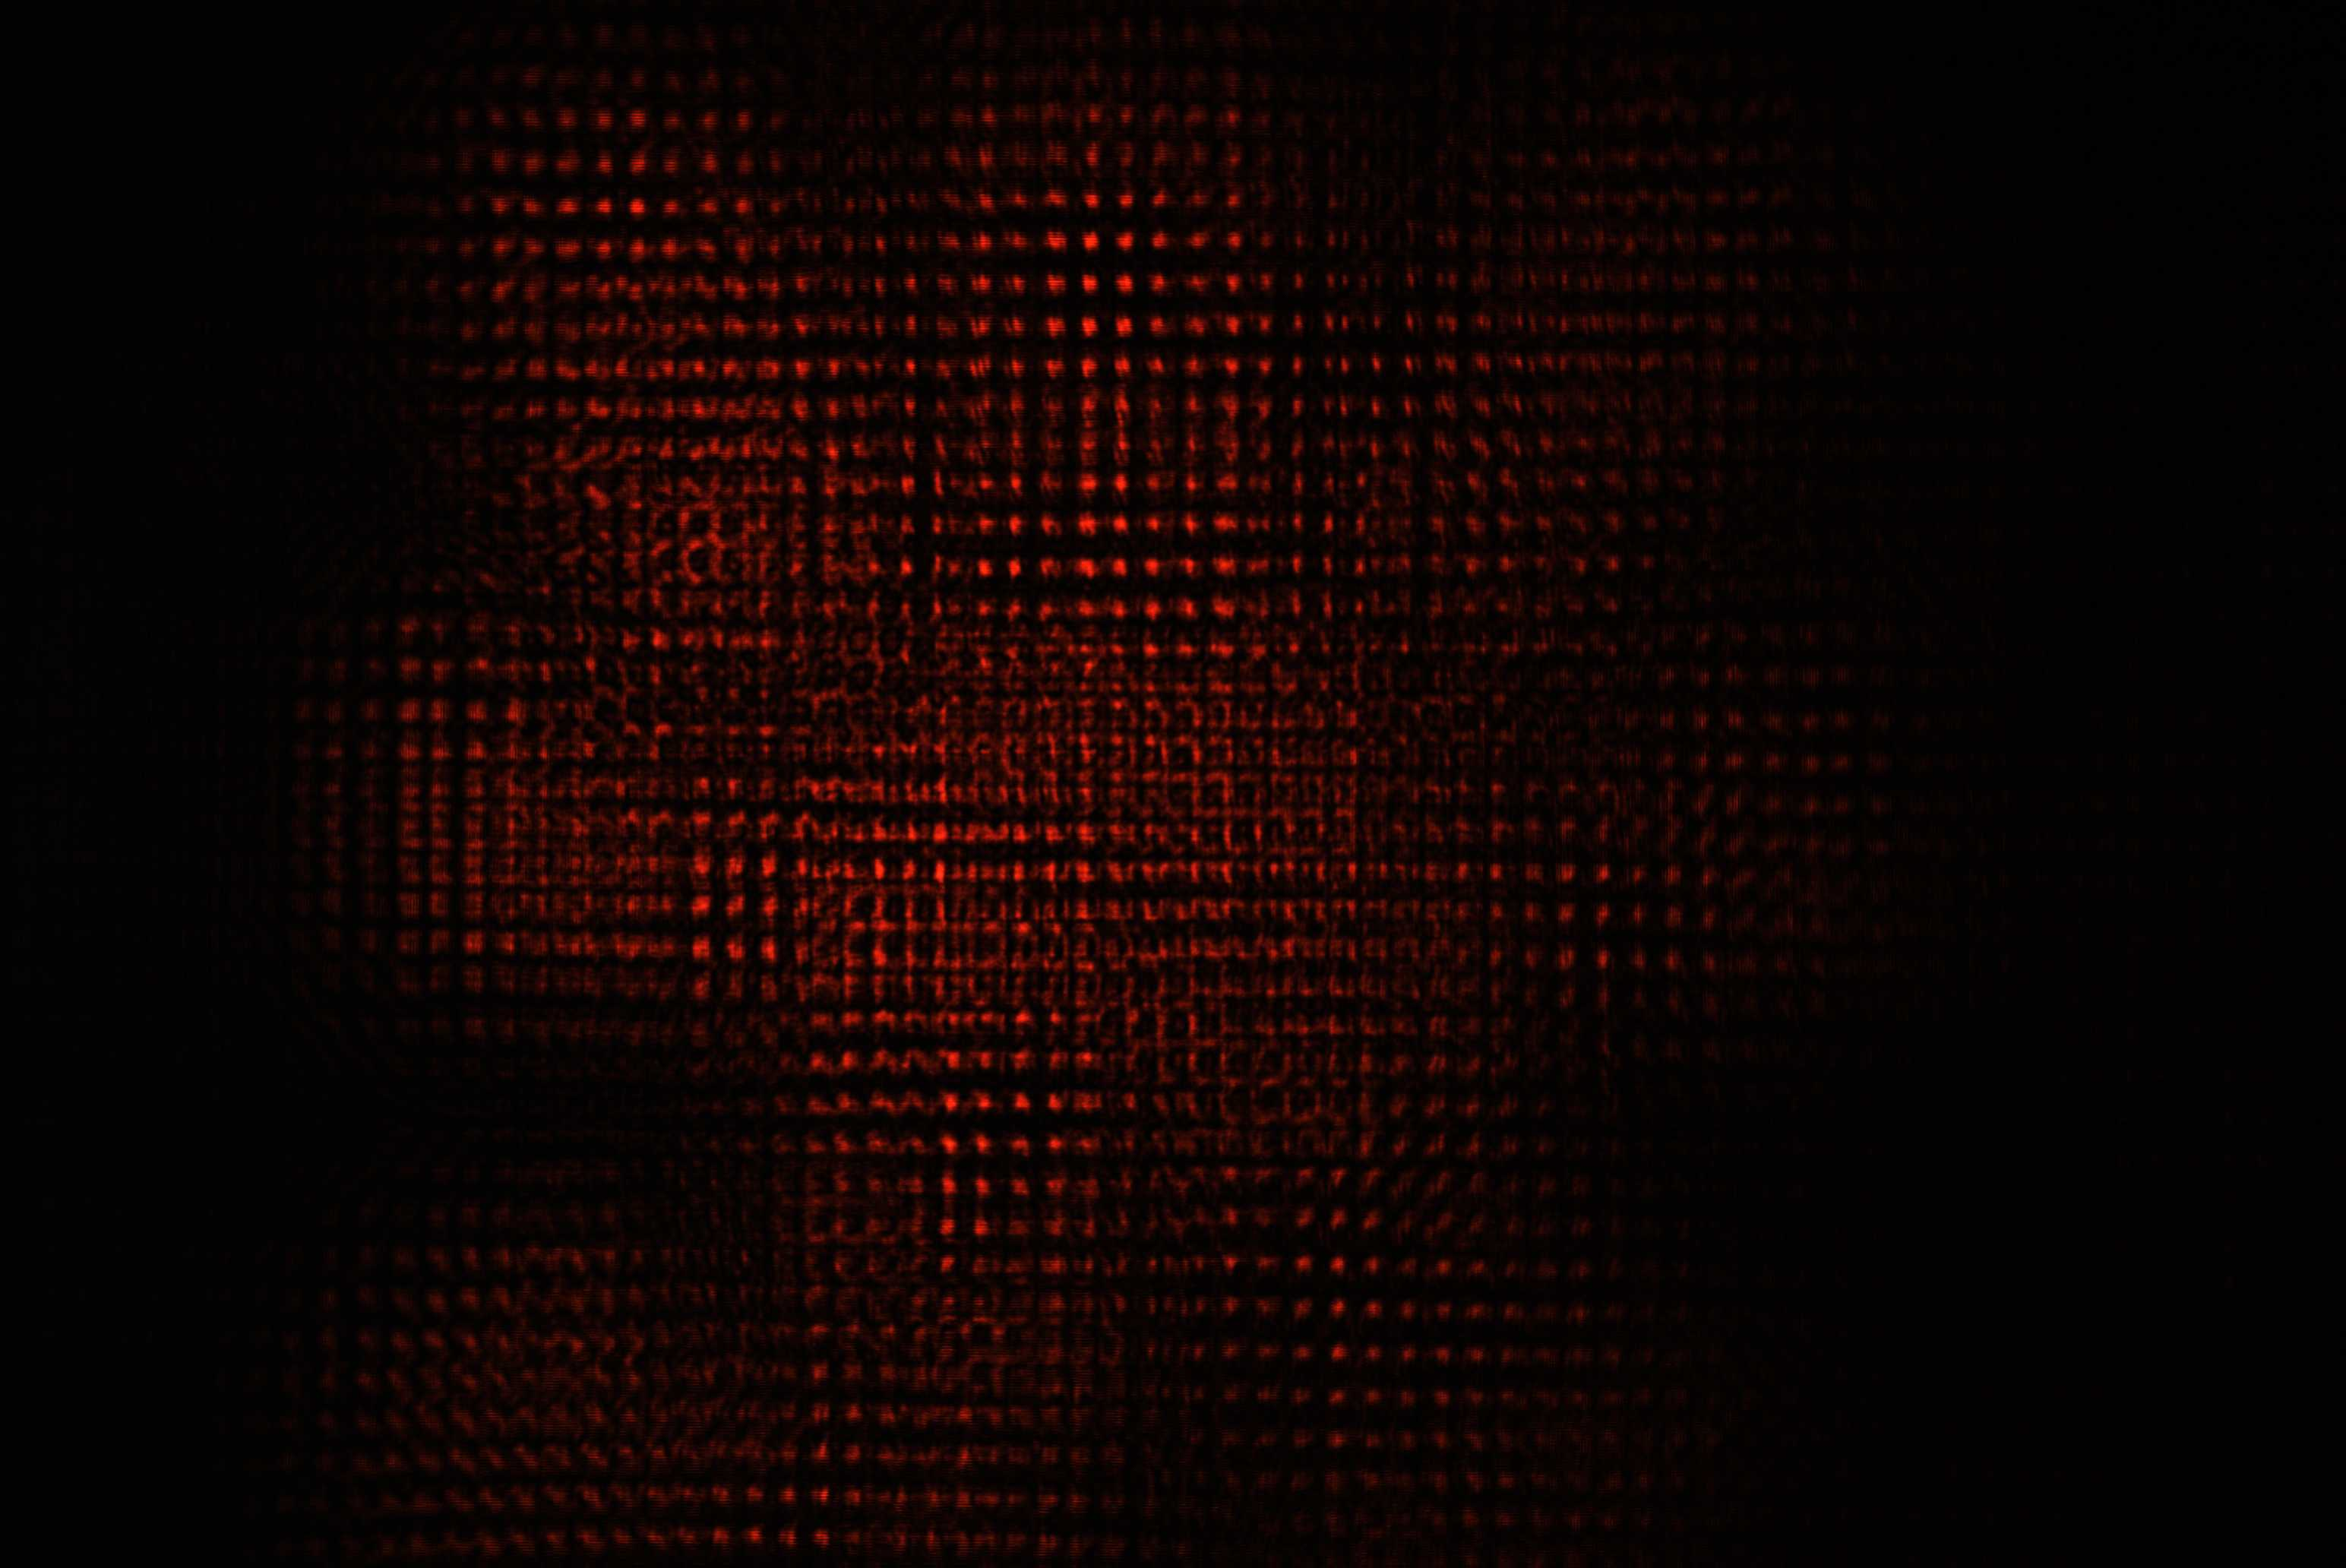
\includegraphics[width=0.3\textwidth]{attachments/fig.3.3.1.2.jpg}
			}

			\subfloat[High-pass]{\label{fig.3.3.1.3}
			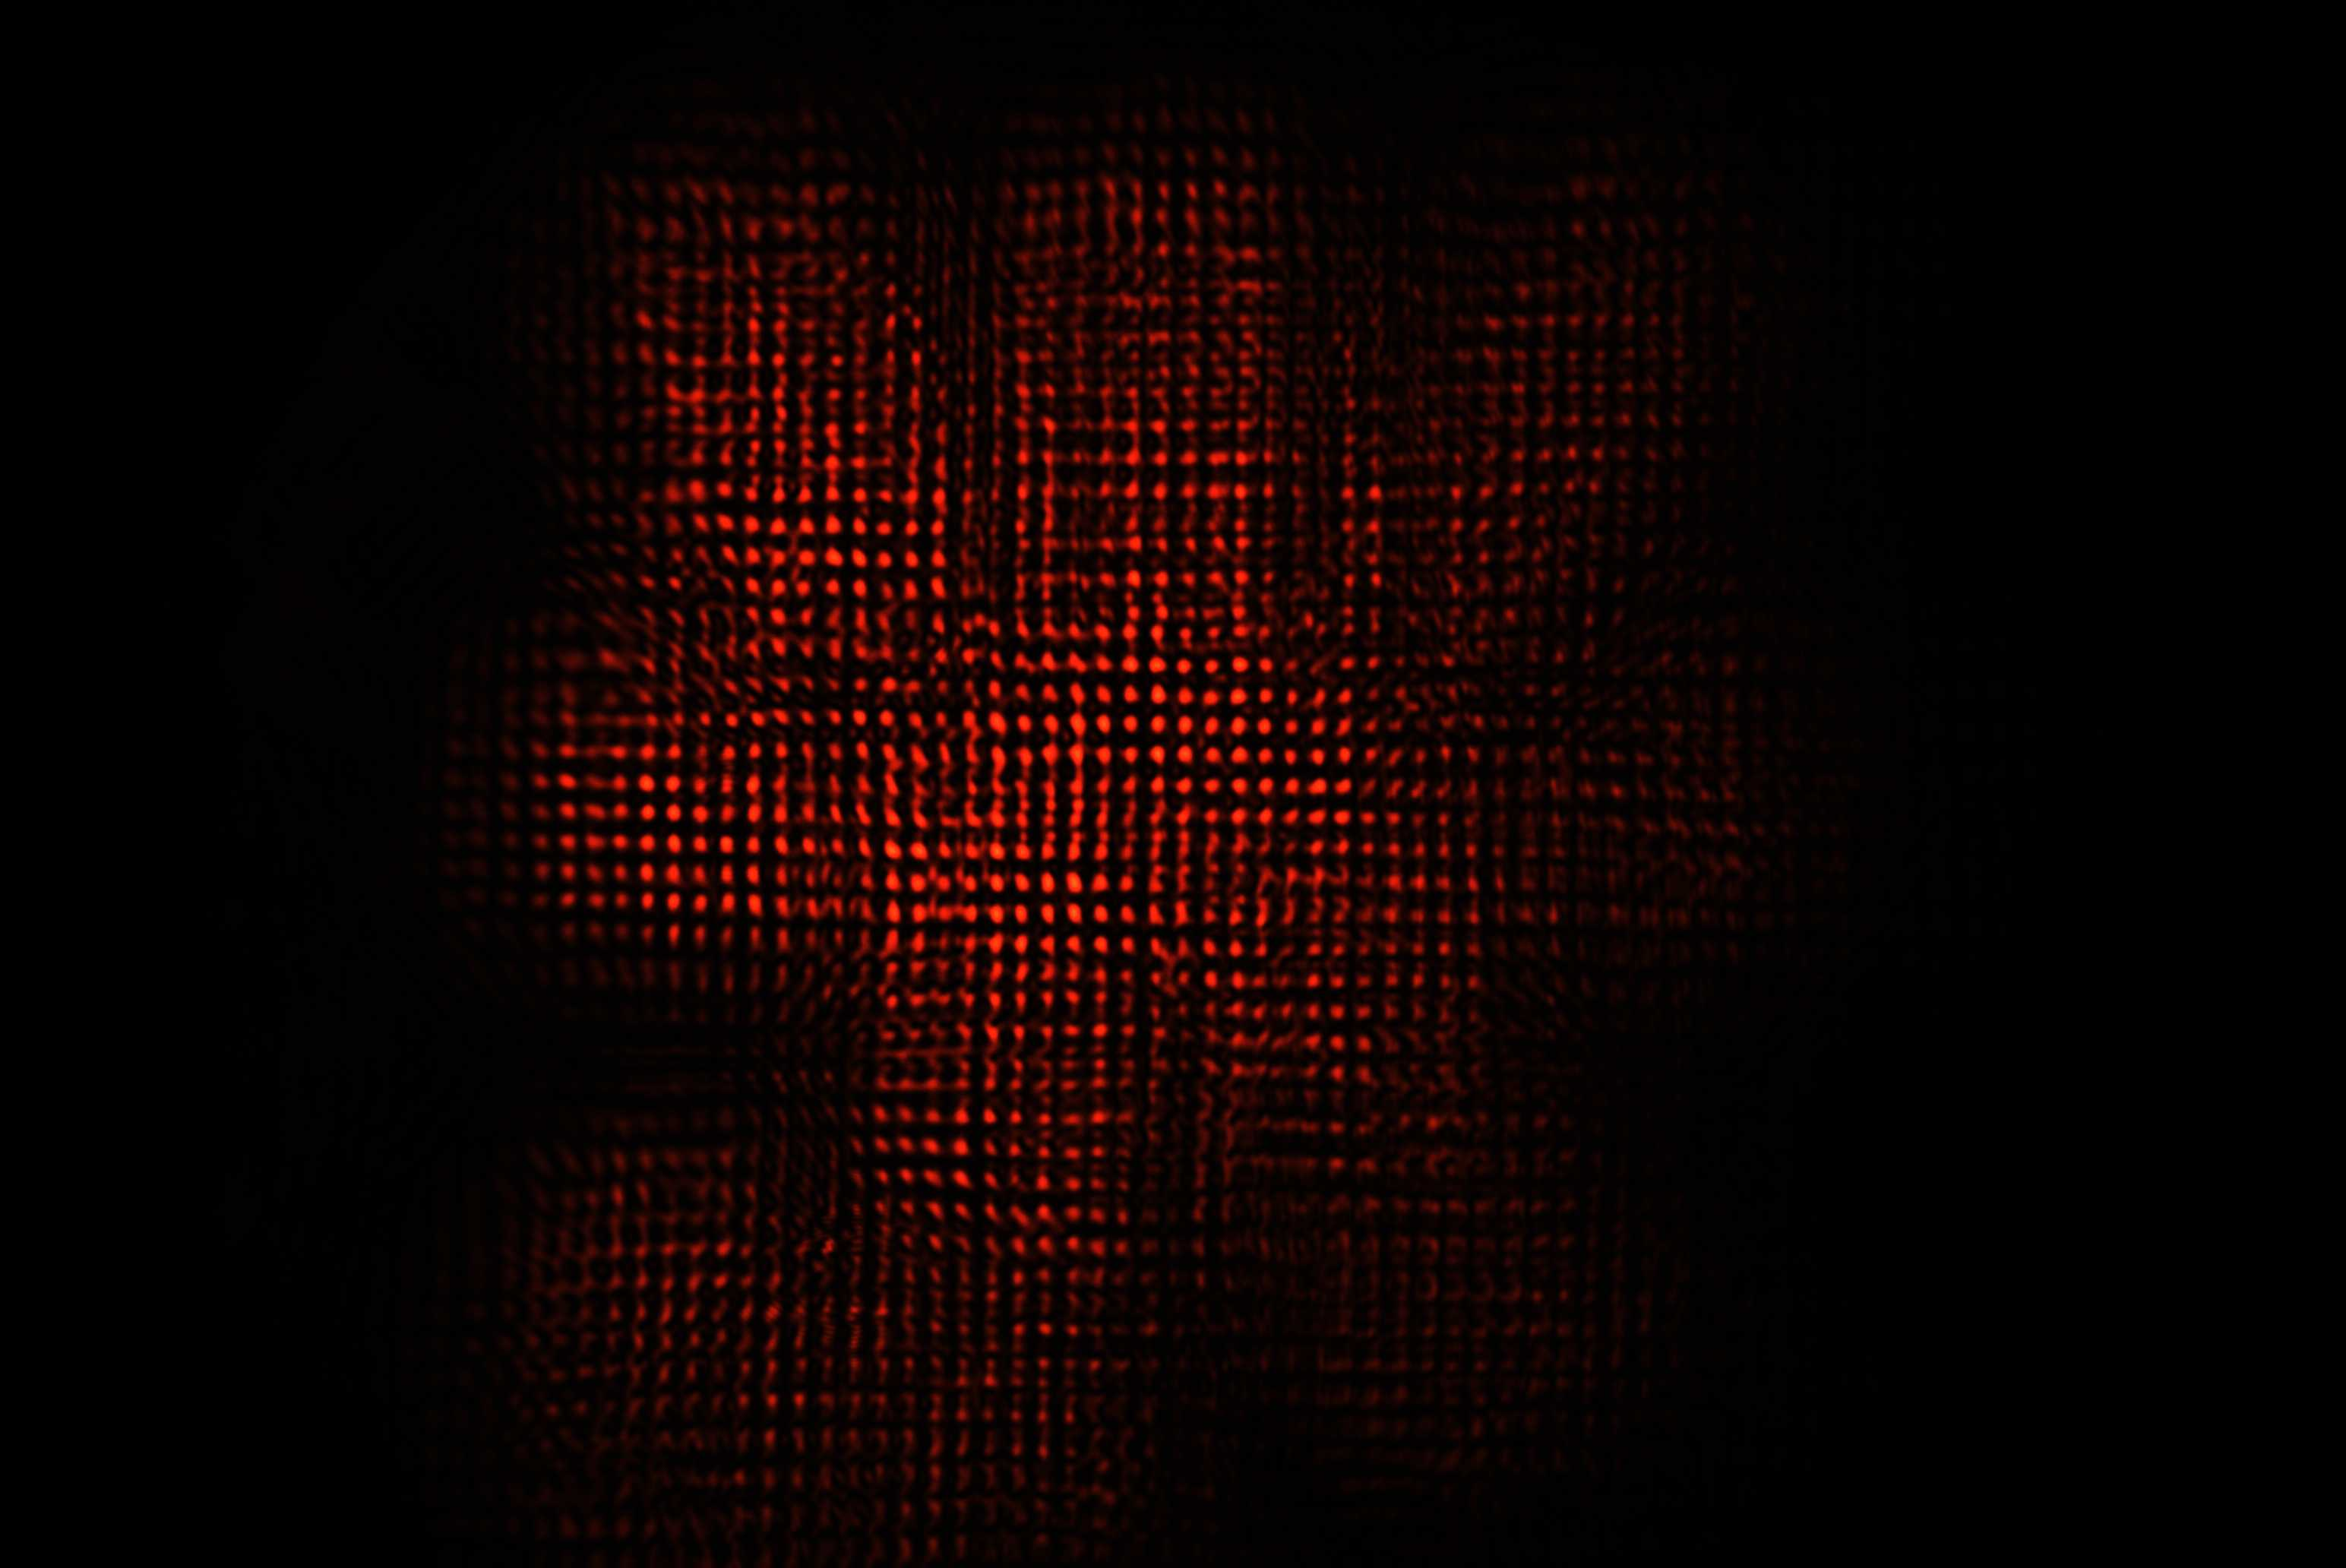
\includegraphics[width=0.3\textwidth]{attachments/fig.3.3.1.3.jpg}
			}		
			\subfloat[Low-pass]{\label{fig.3.3.1.4}
			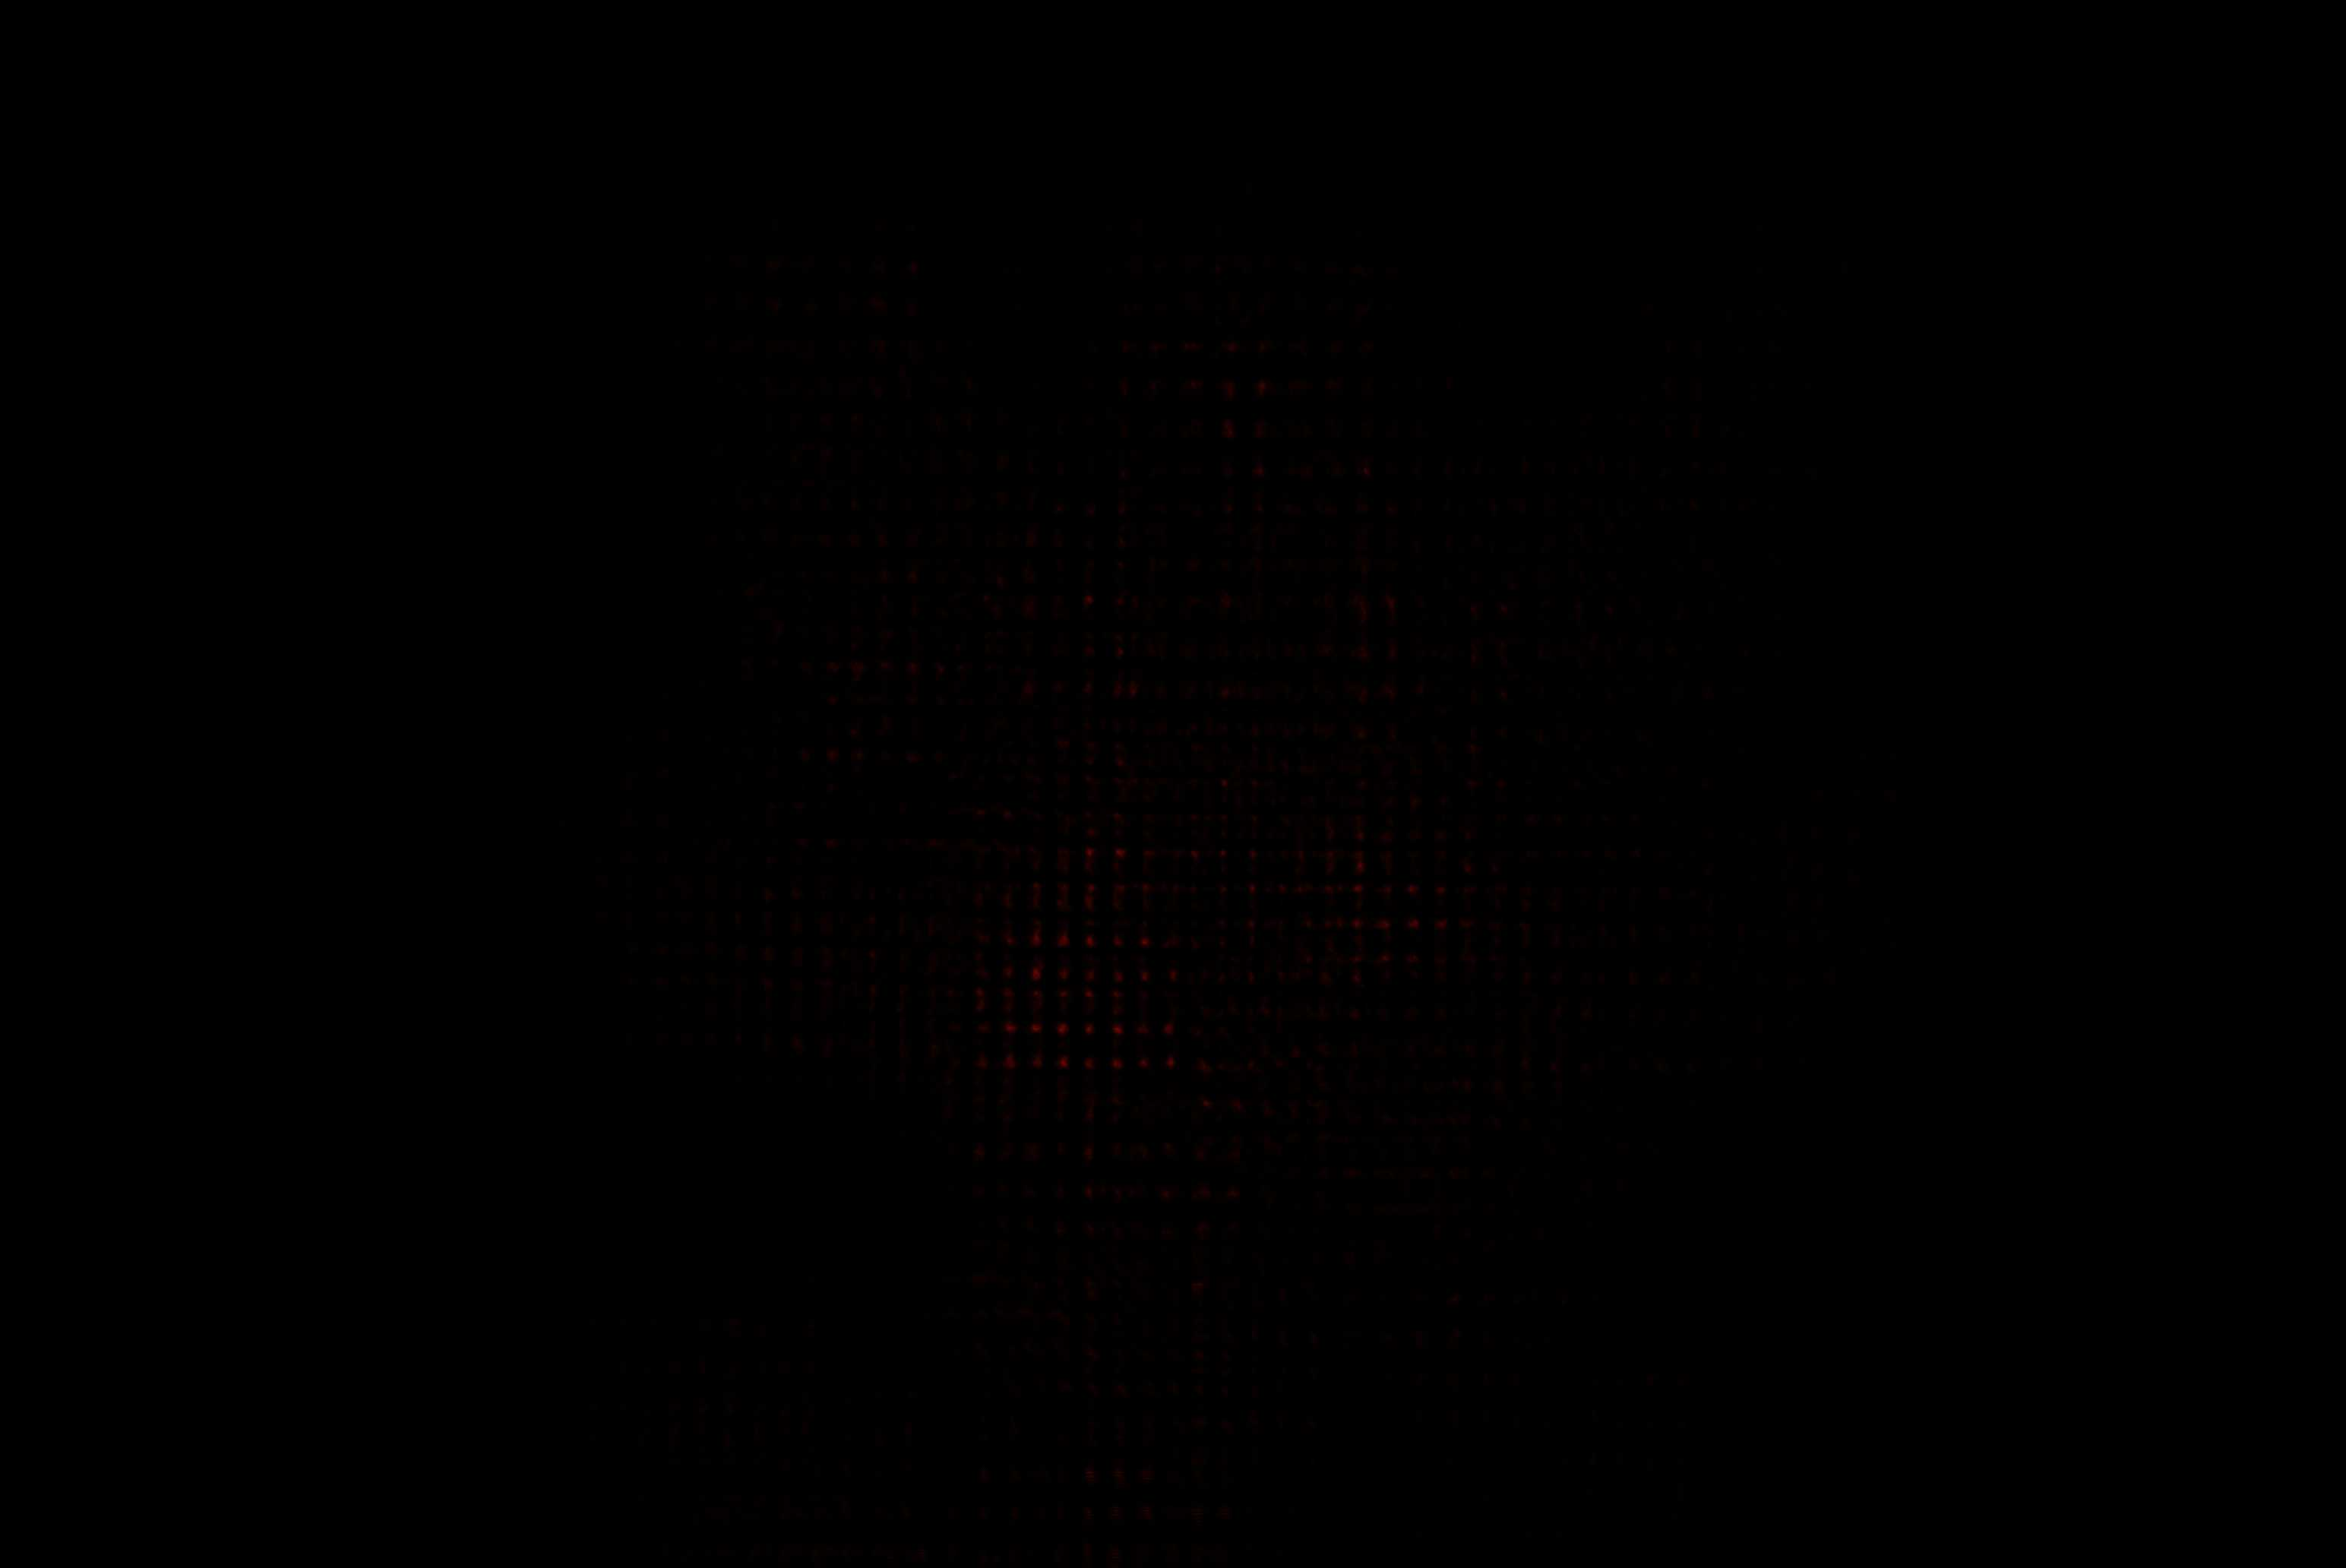
\includegraphics[width=0.3\textwidth]{attachments/fig.3.3.1.4.jpg}
			}
			\caption{\textbf{High-pass and low-pass filtering}}
		\end{figure*}

		\begin{figure*}[htbp]
			\centering
			\subfloat[Object: 128Tx96T 2D grating]{\label{fig.3.3.2.1}
			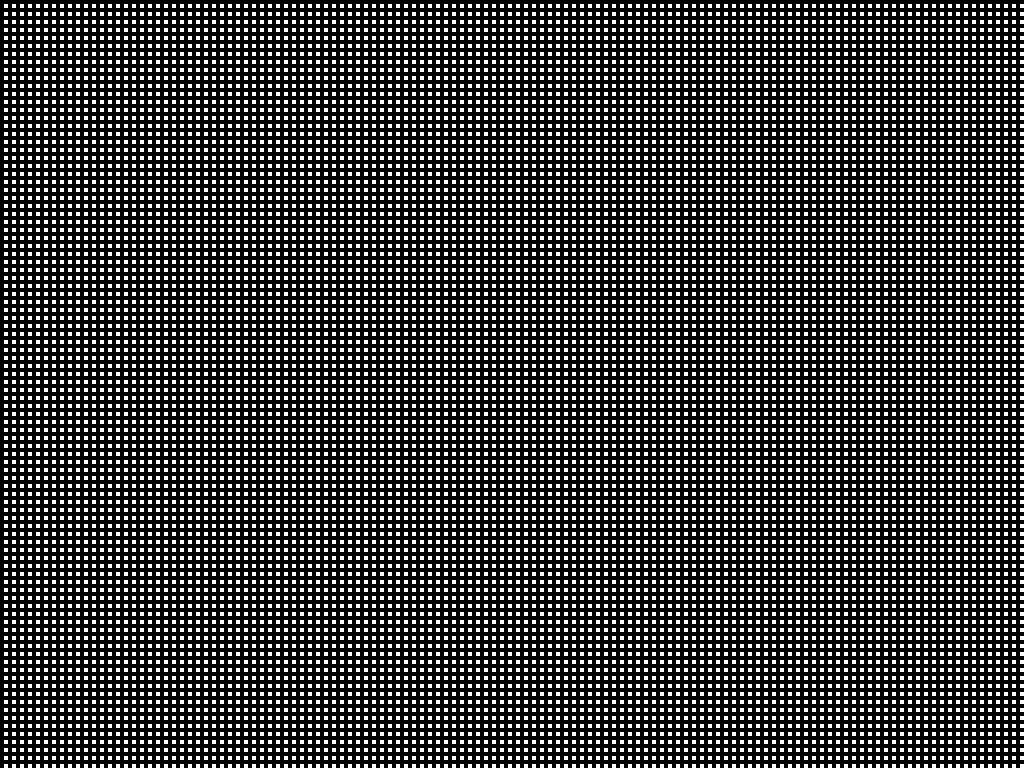
\includegraphics[width=0.24\textwidth]{attachments/fig.3.3.2.1.jpg}
			}		
			\subfloat[Spatial spectrum]{\label{fig.3.3.2.2}
			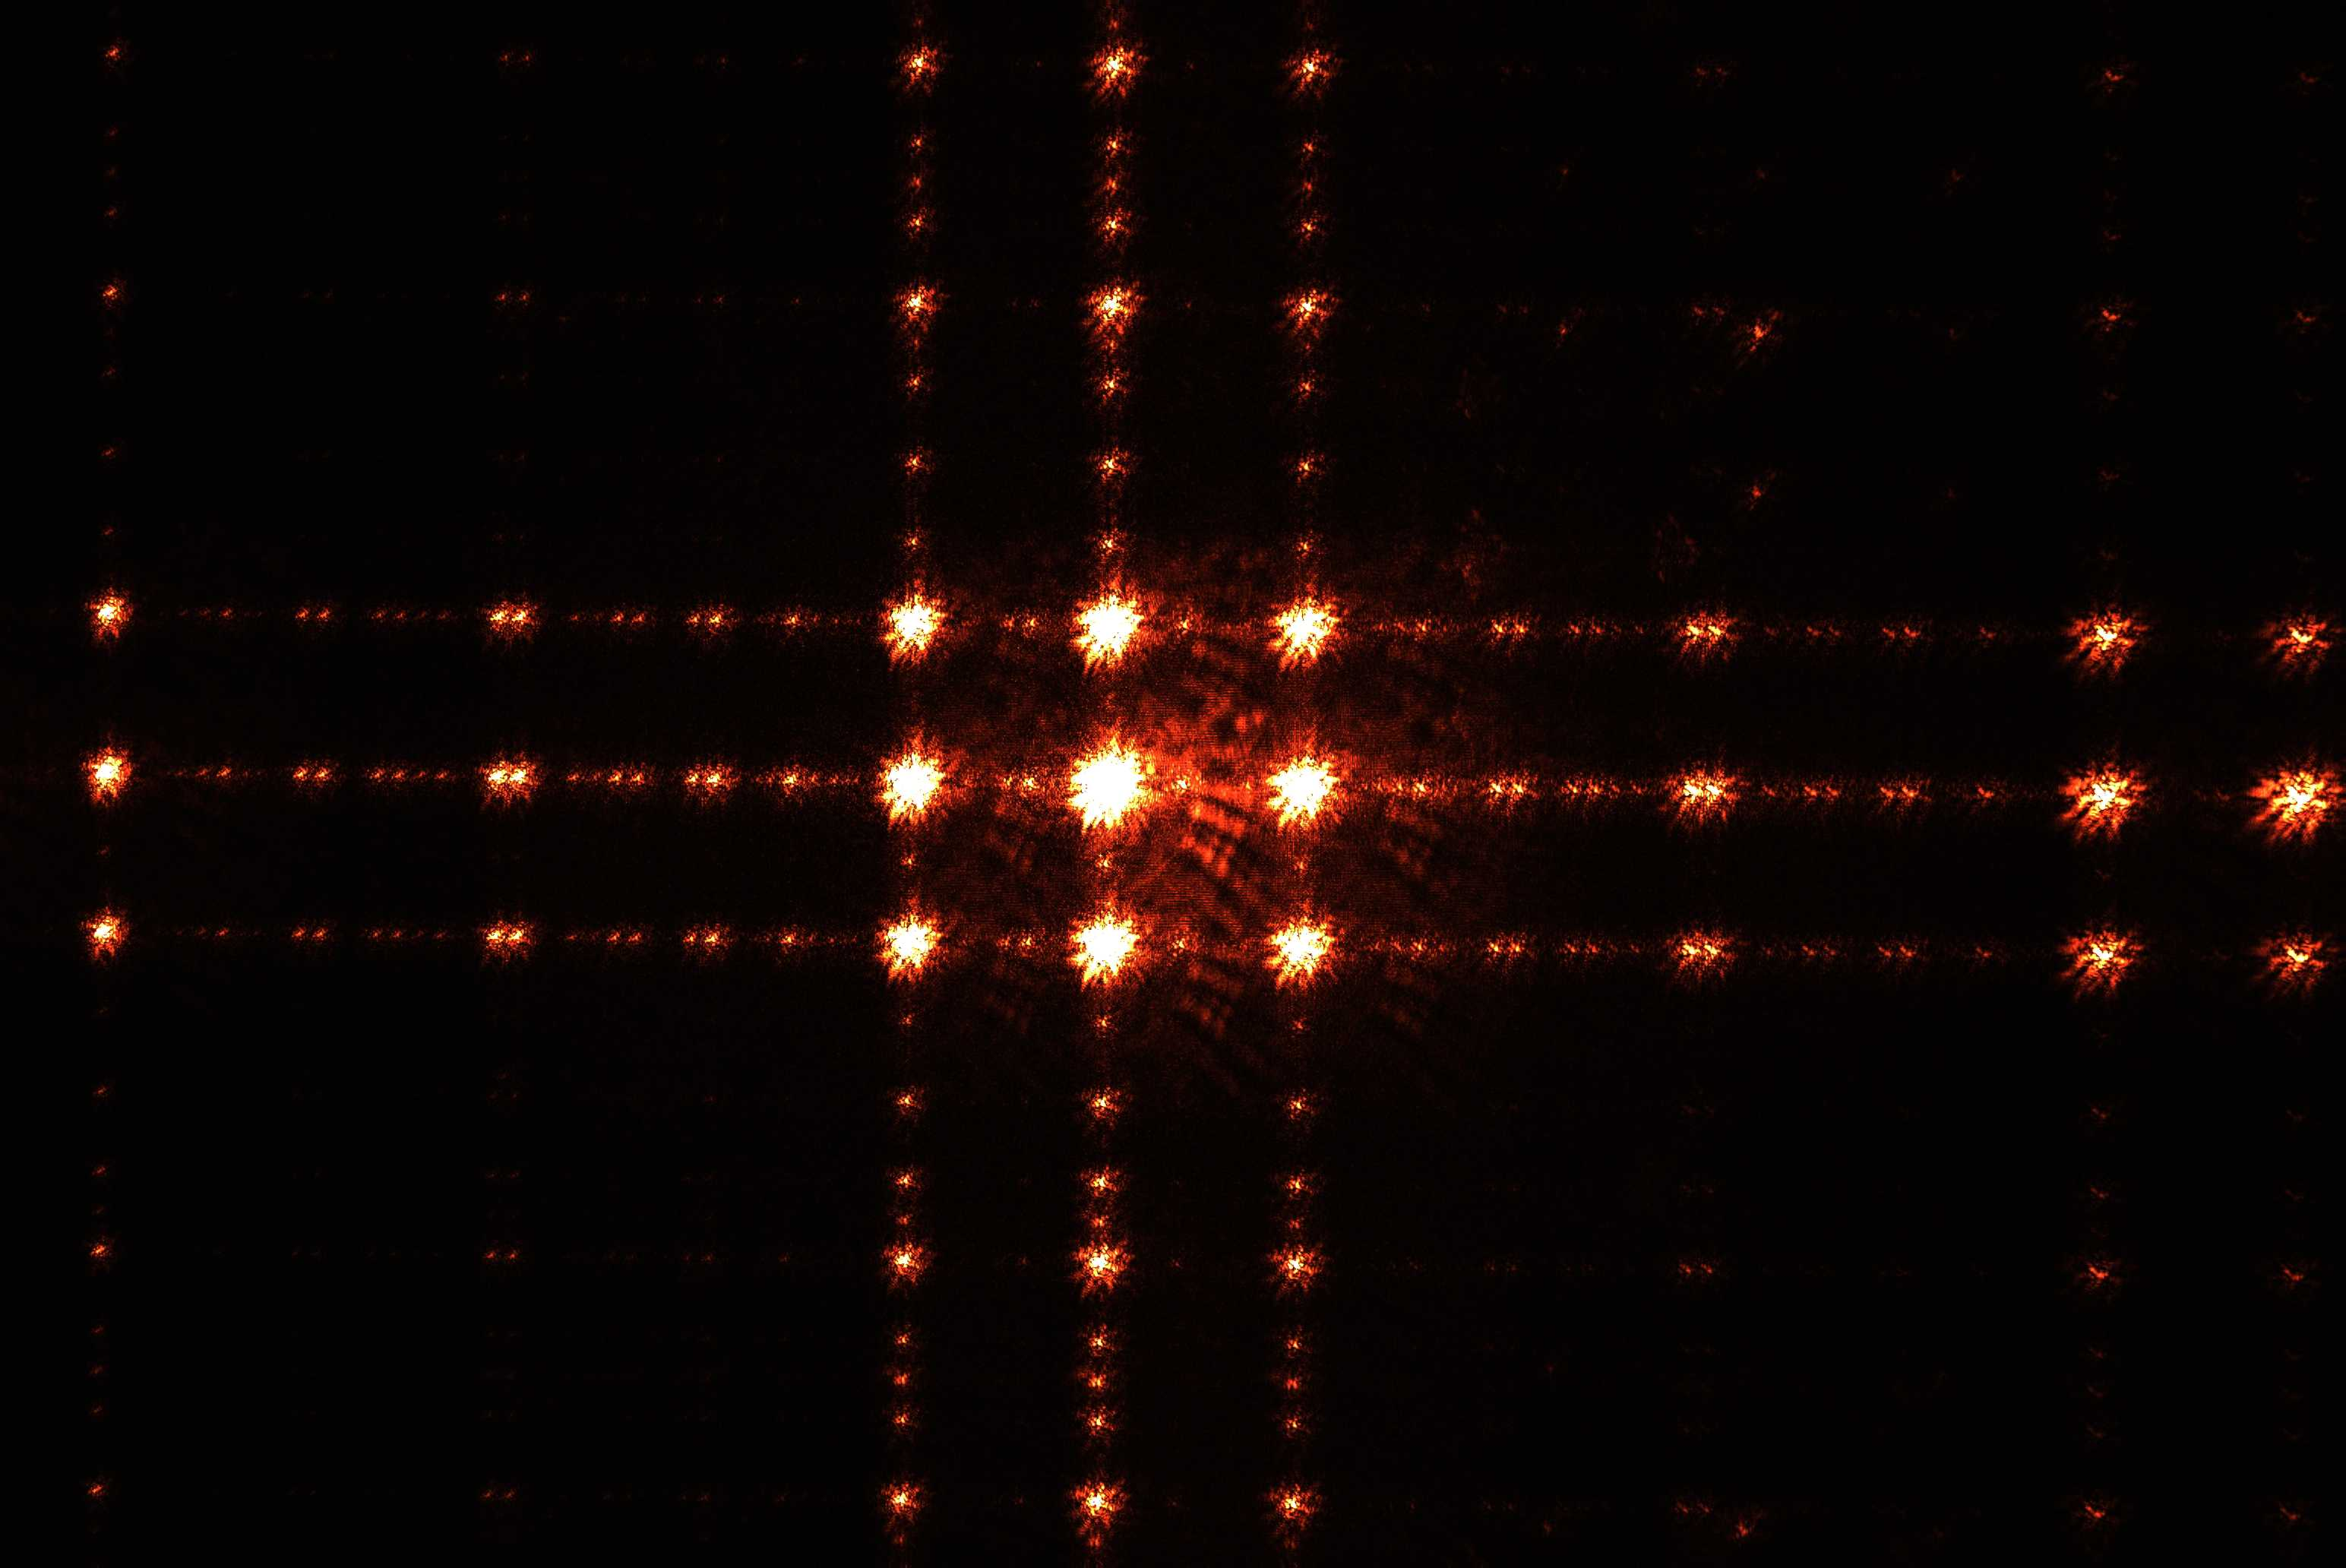
\includegraphics[width=0.24\textwidth]{attachments/fig.3.3.2.2.jpg}
			}

			\subfloat[$45^o$]{\label{fig.3.3.2.3}
			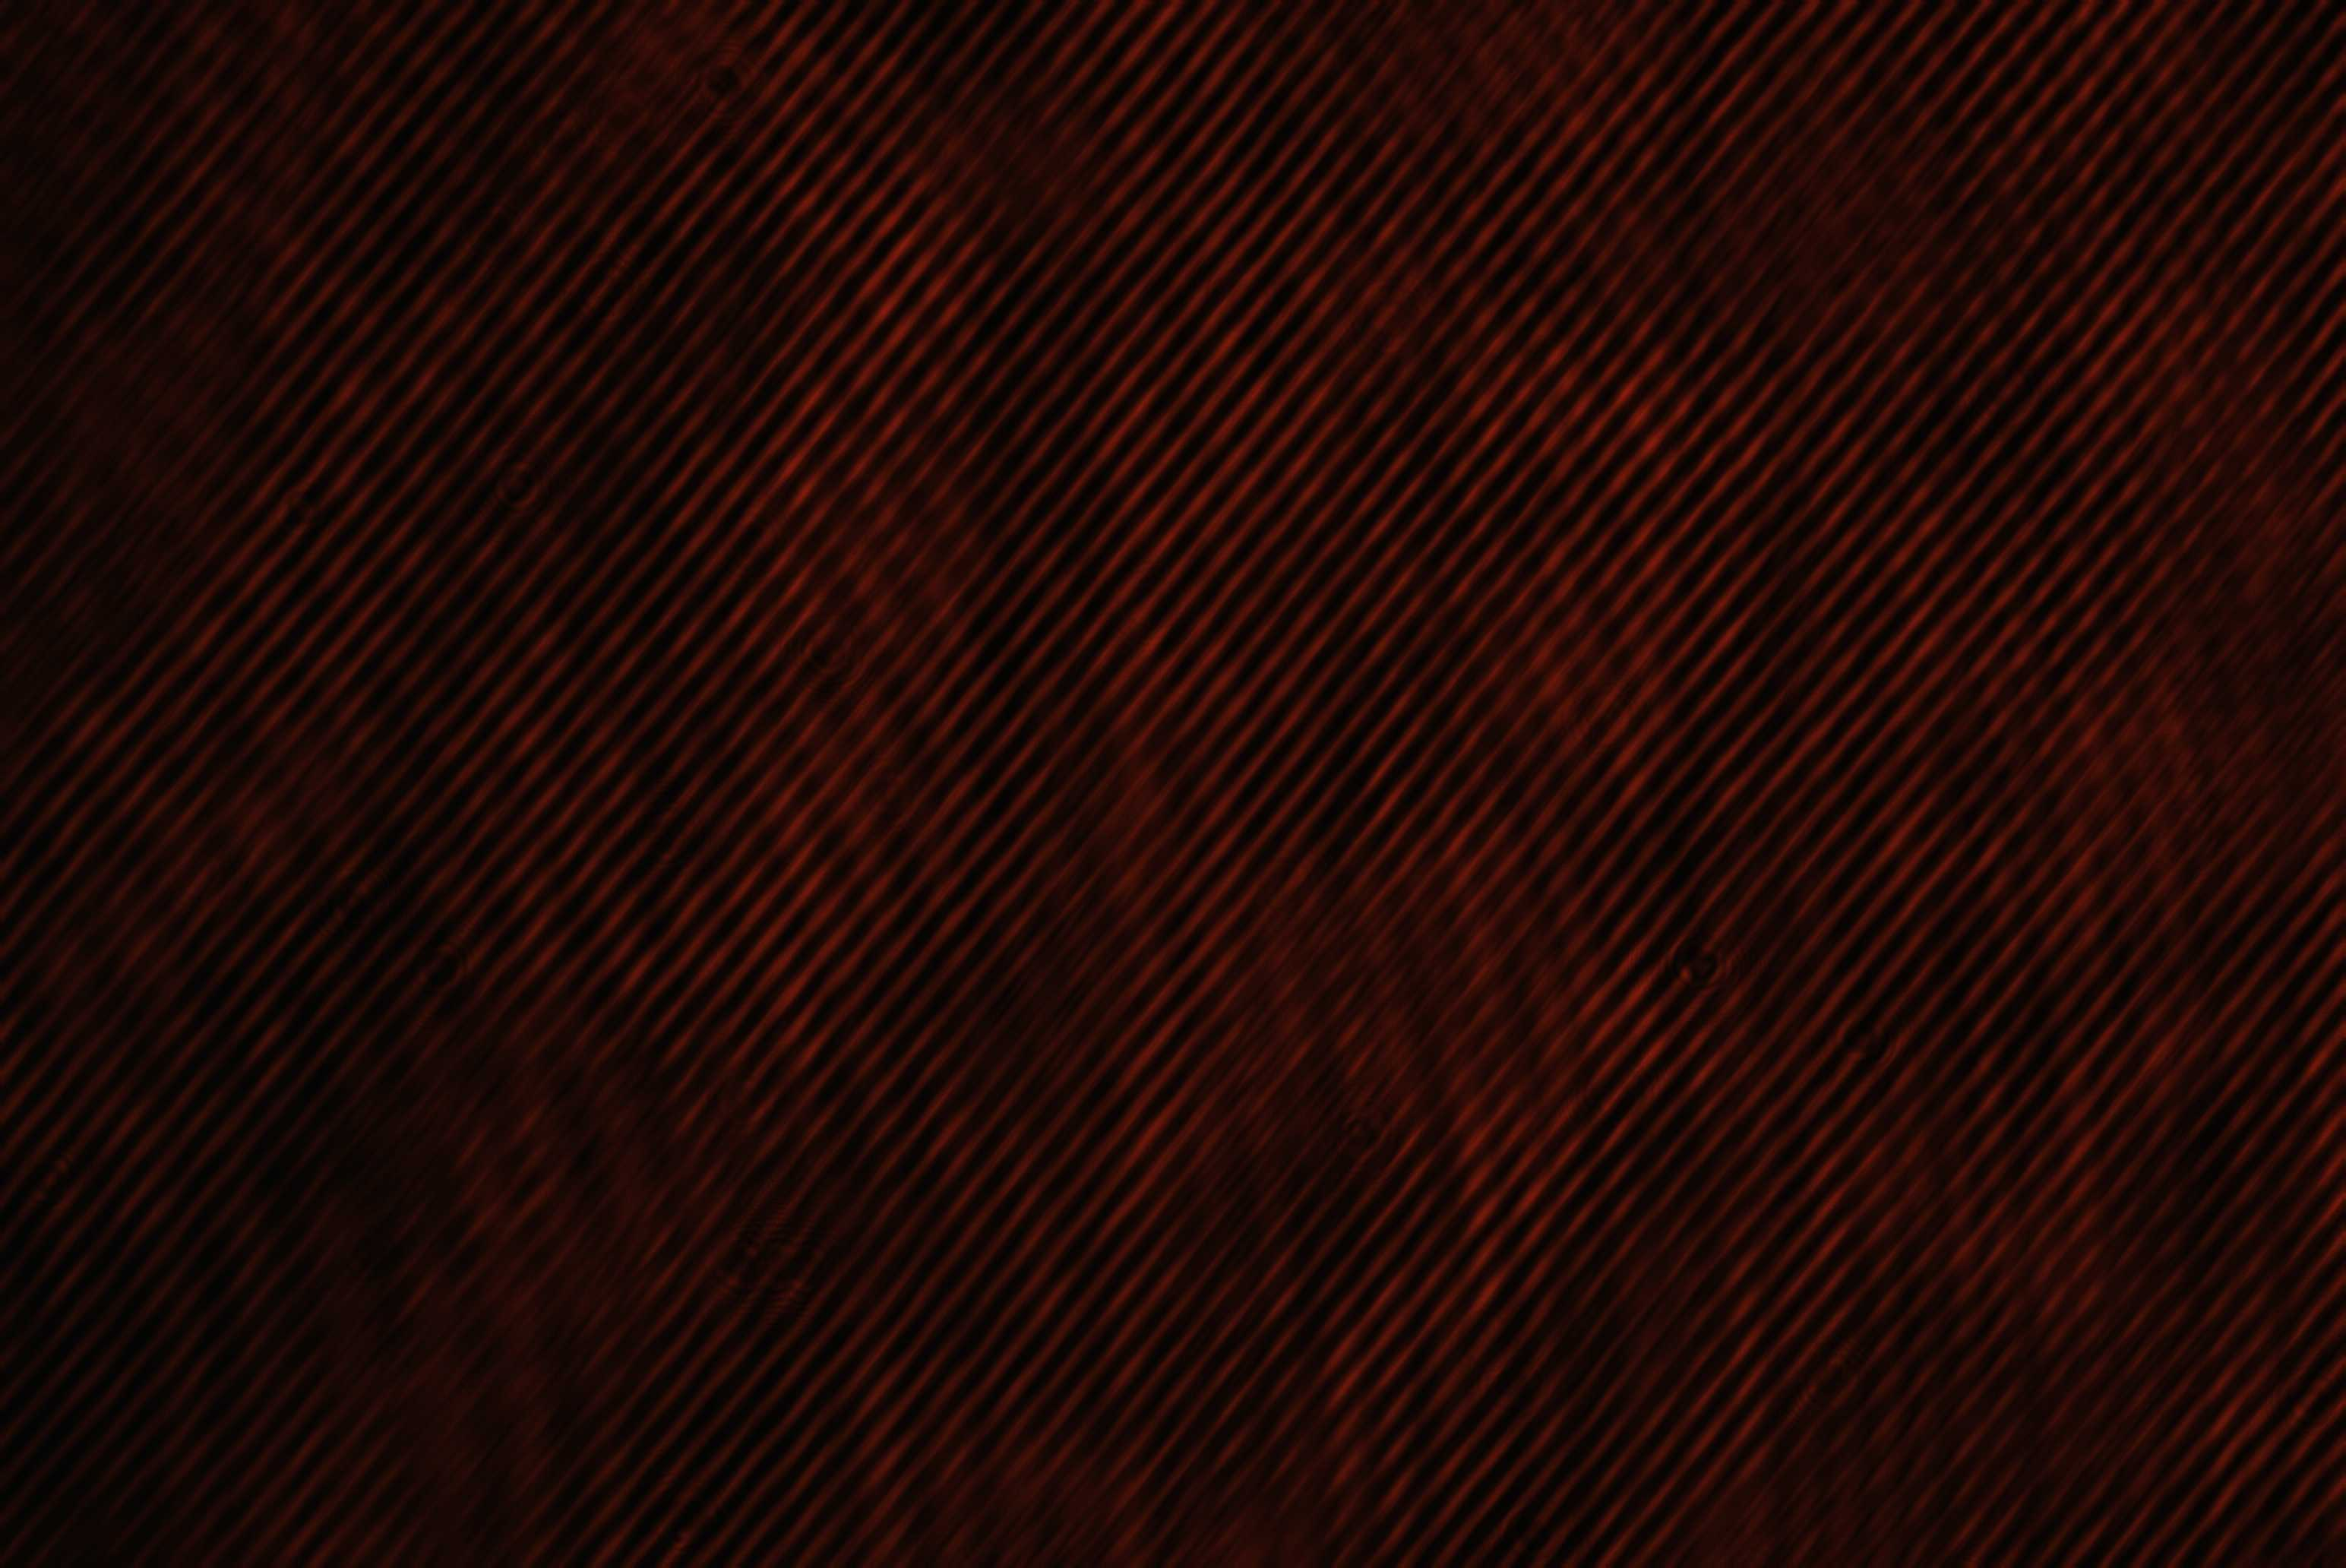
\includegraphics[width=0.24\textwidth]{attachments/fig.3.3.2.3.jpg}
			}		
			\subfloat[$90^o$]{\label{fig.3.3.2.4}
			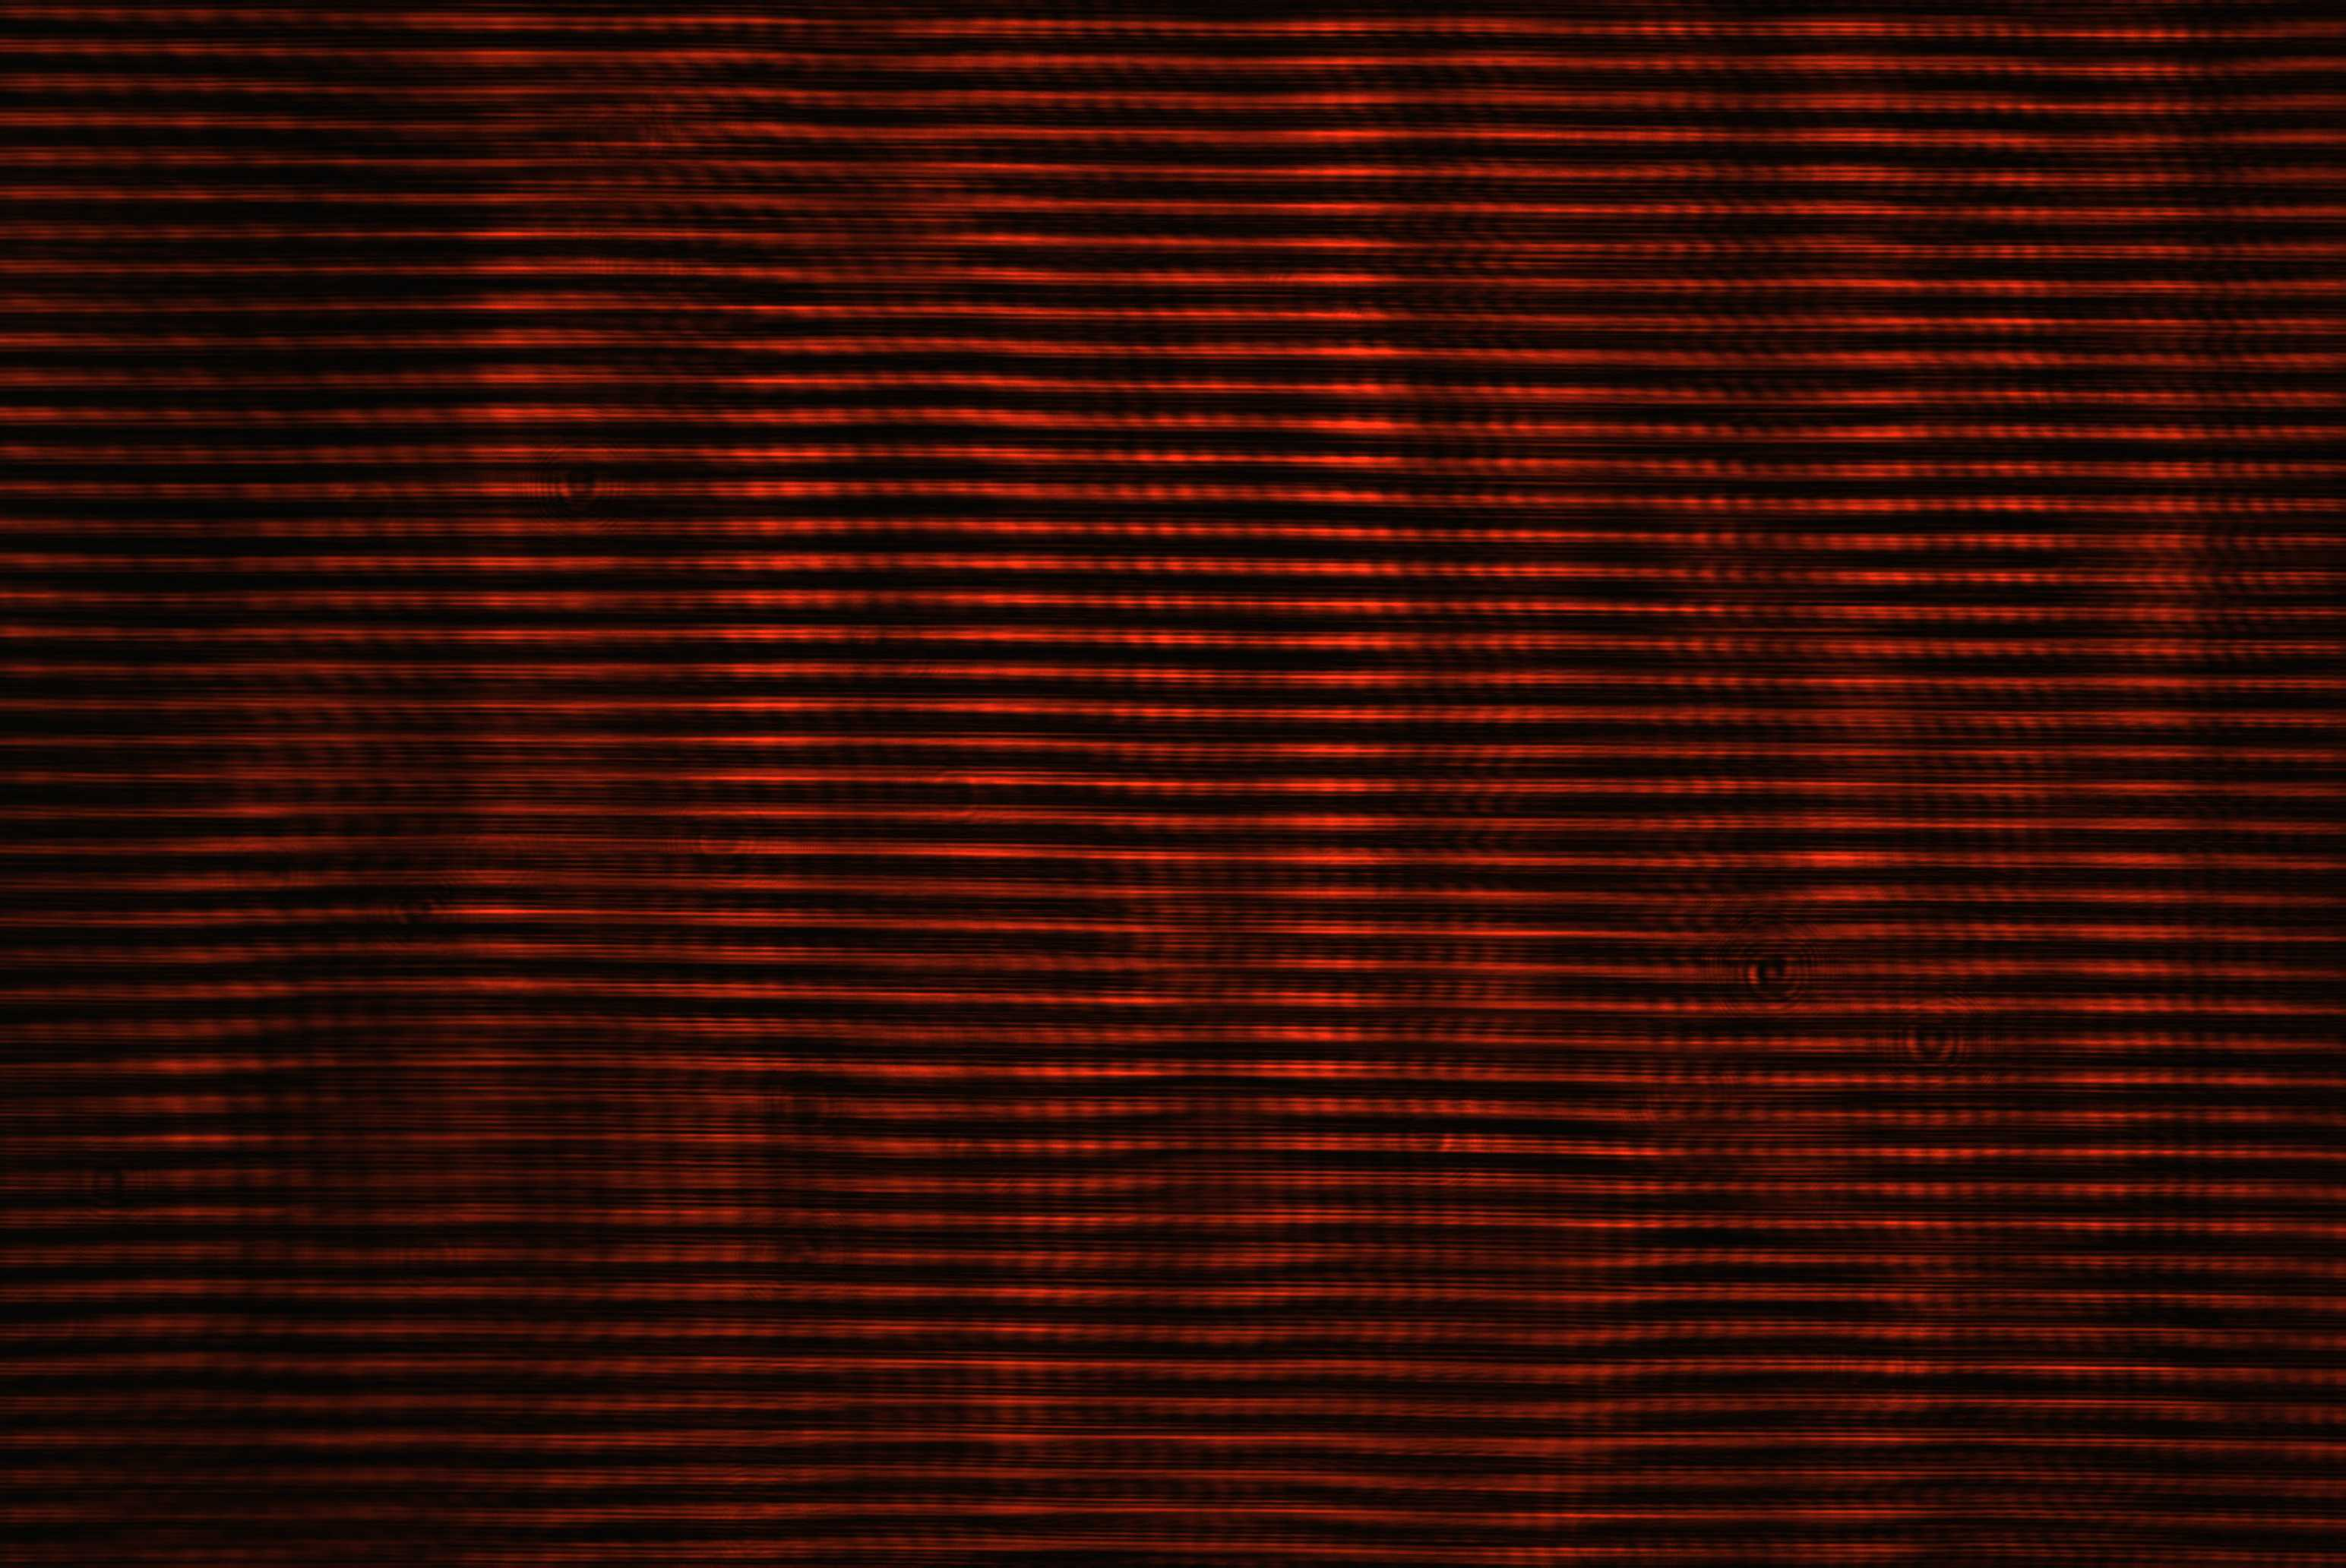
\includegraphics[width=0.24\textwidth]{attachments/fig.3.3.2.4.jpg}
			}
			\subfloat[$135^o$]{\label{fig.3.3.2.5}
			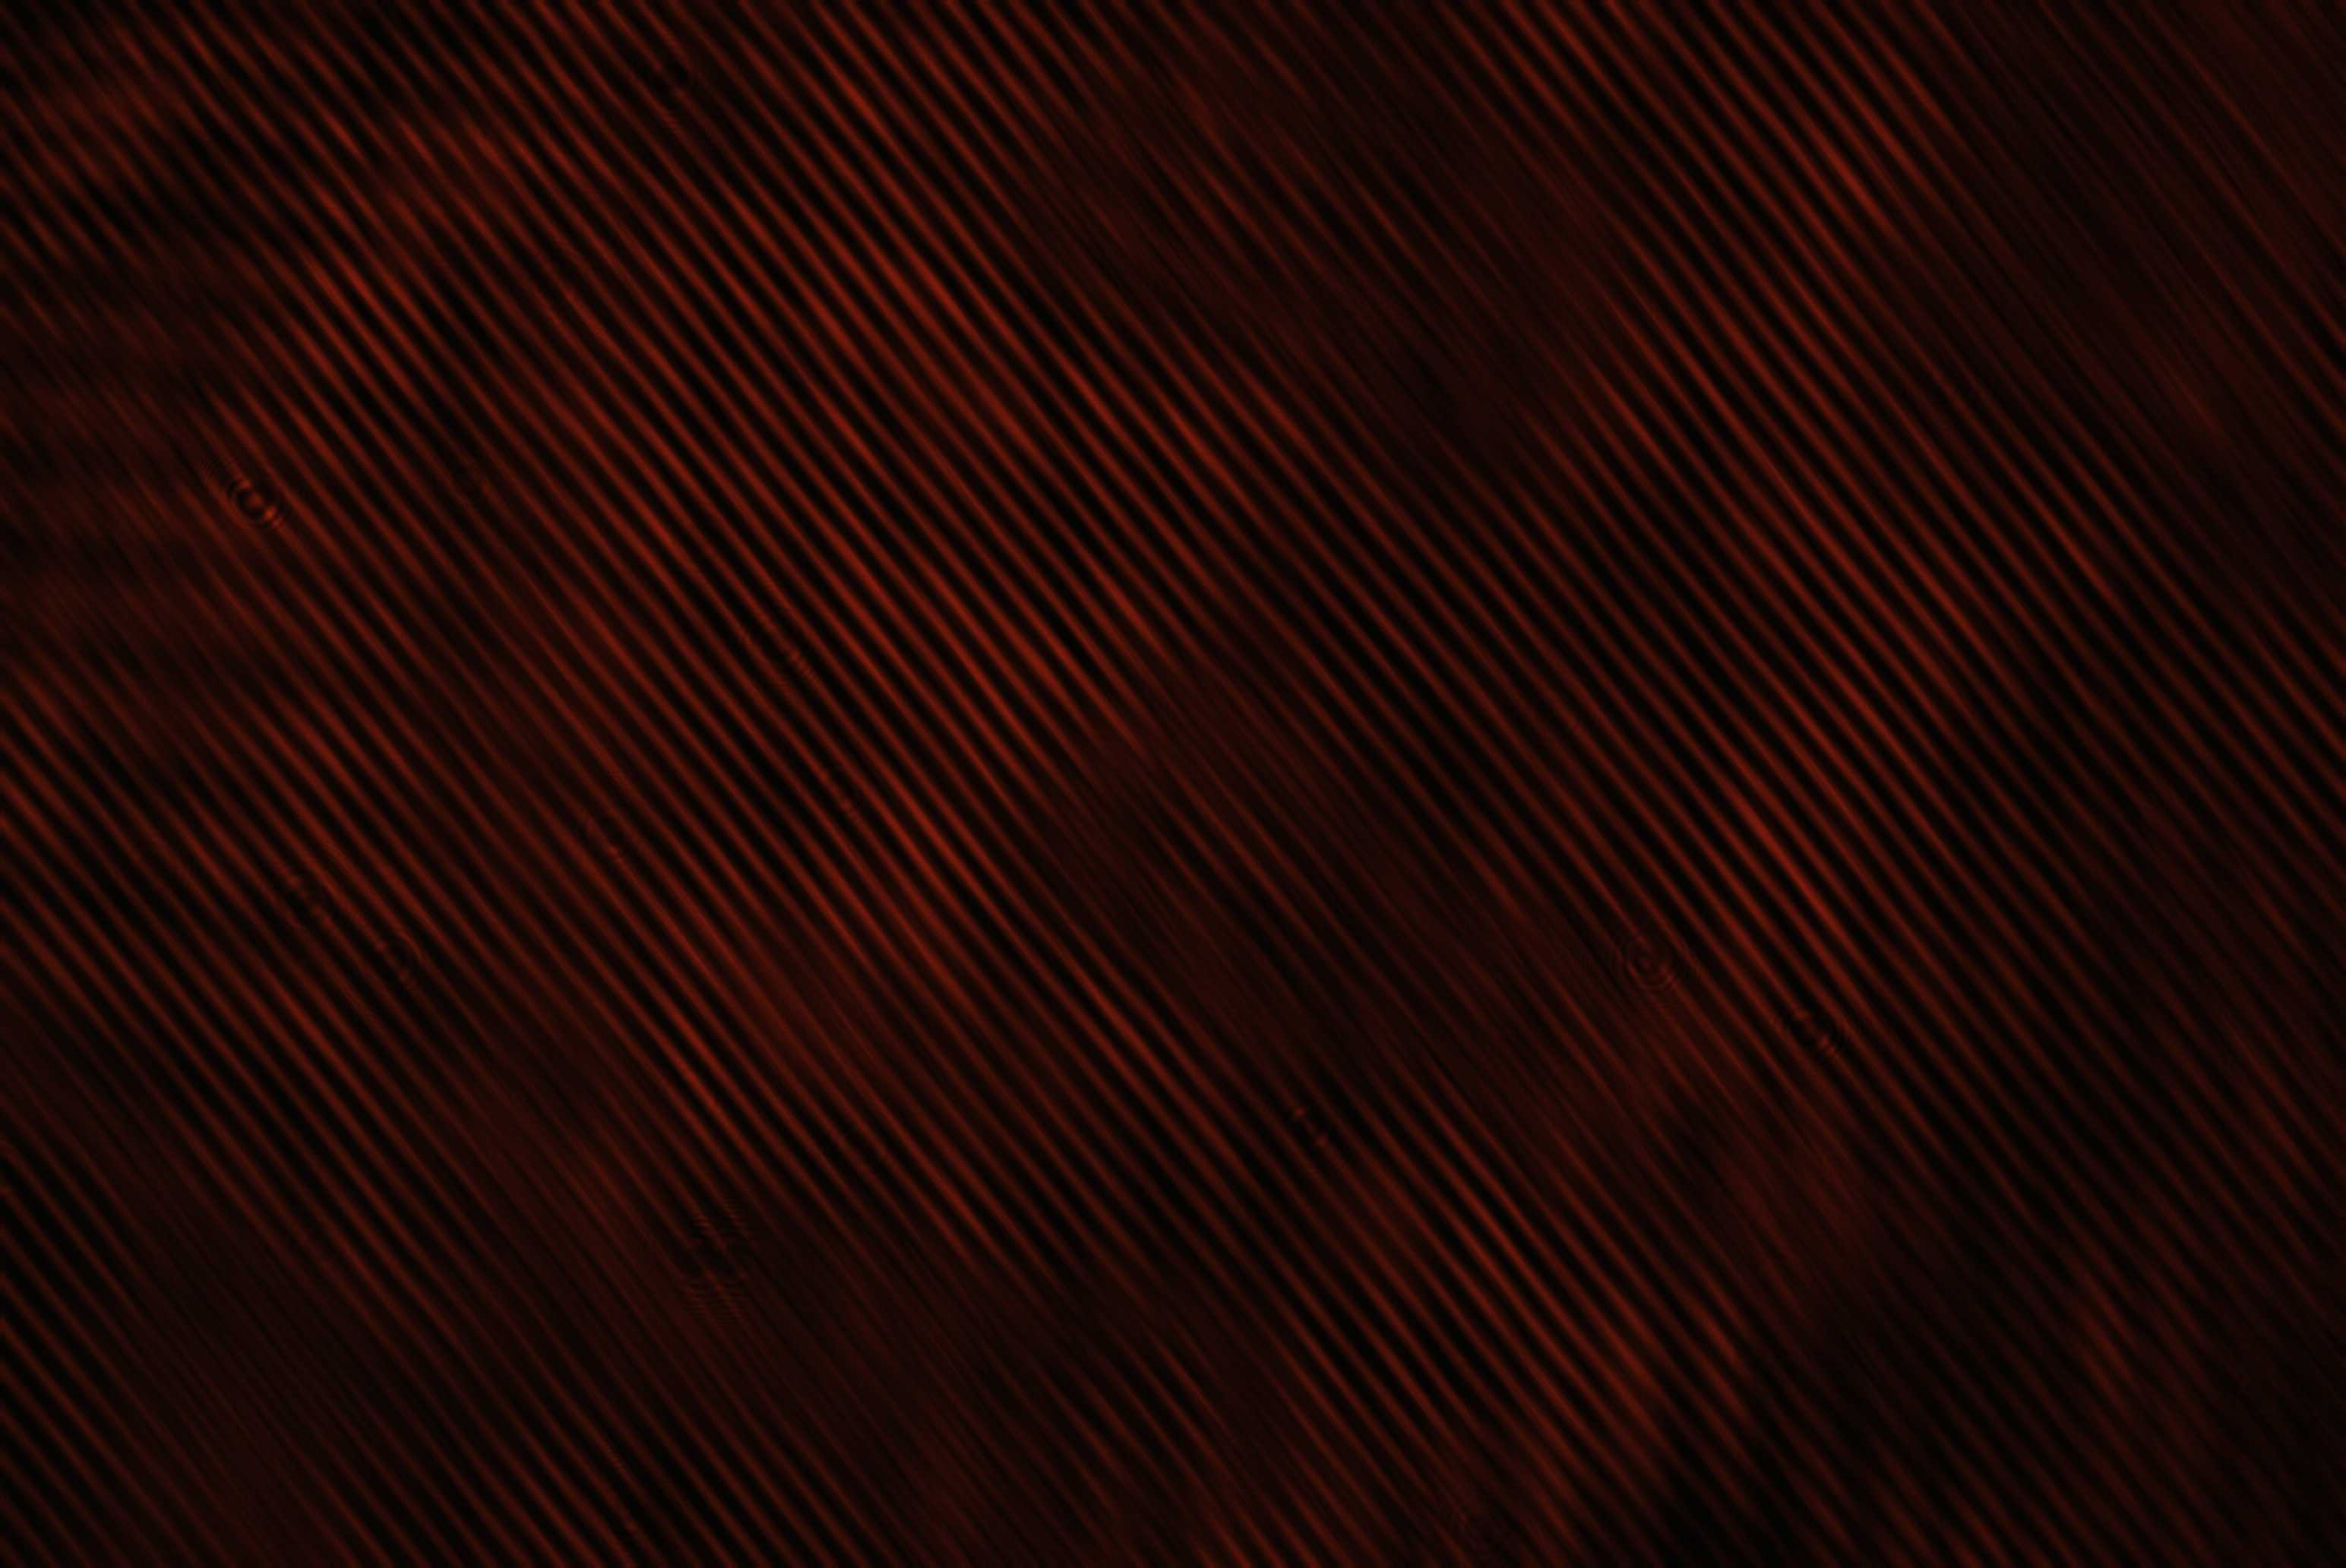
\includegraphics[width=0.24\textwidth]{attachments/fig.3.3.2.5.jpg}
			}		
			\subfloat[$180^o$]{\label{fig.3.3.2.6}
			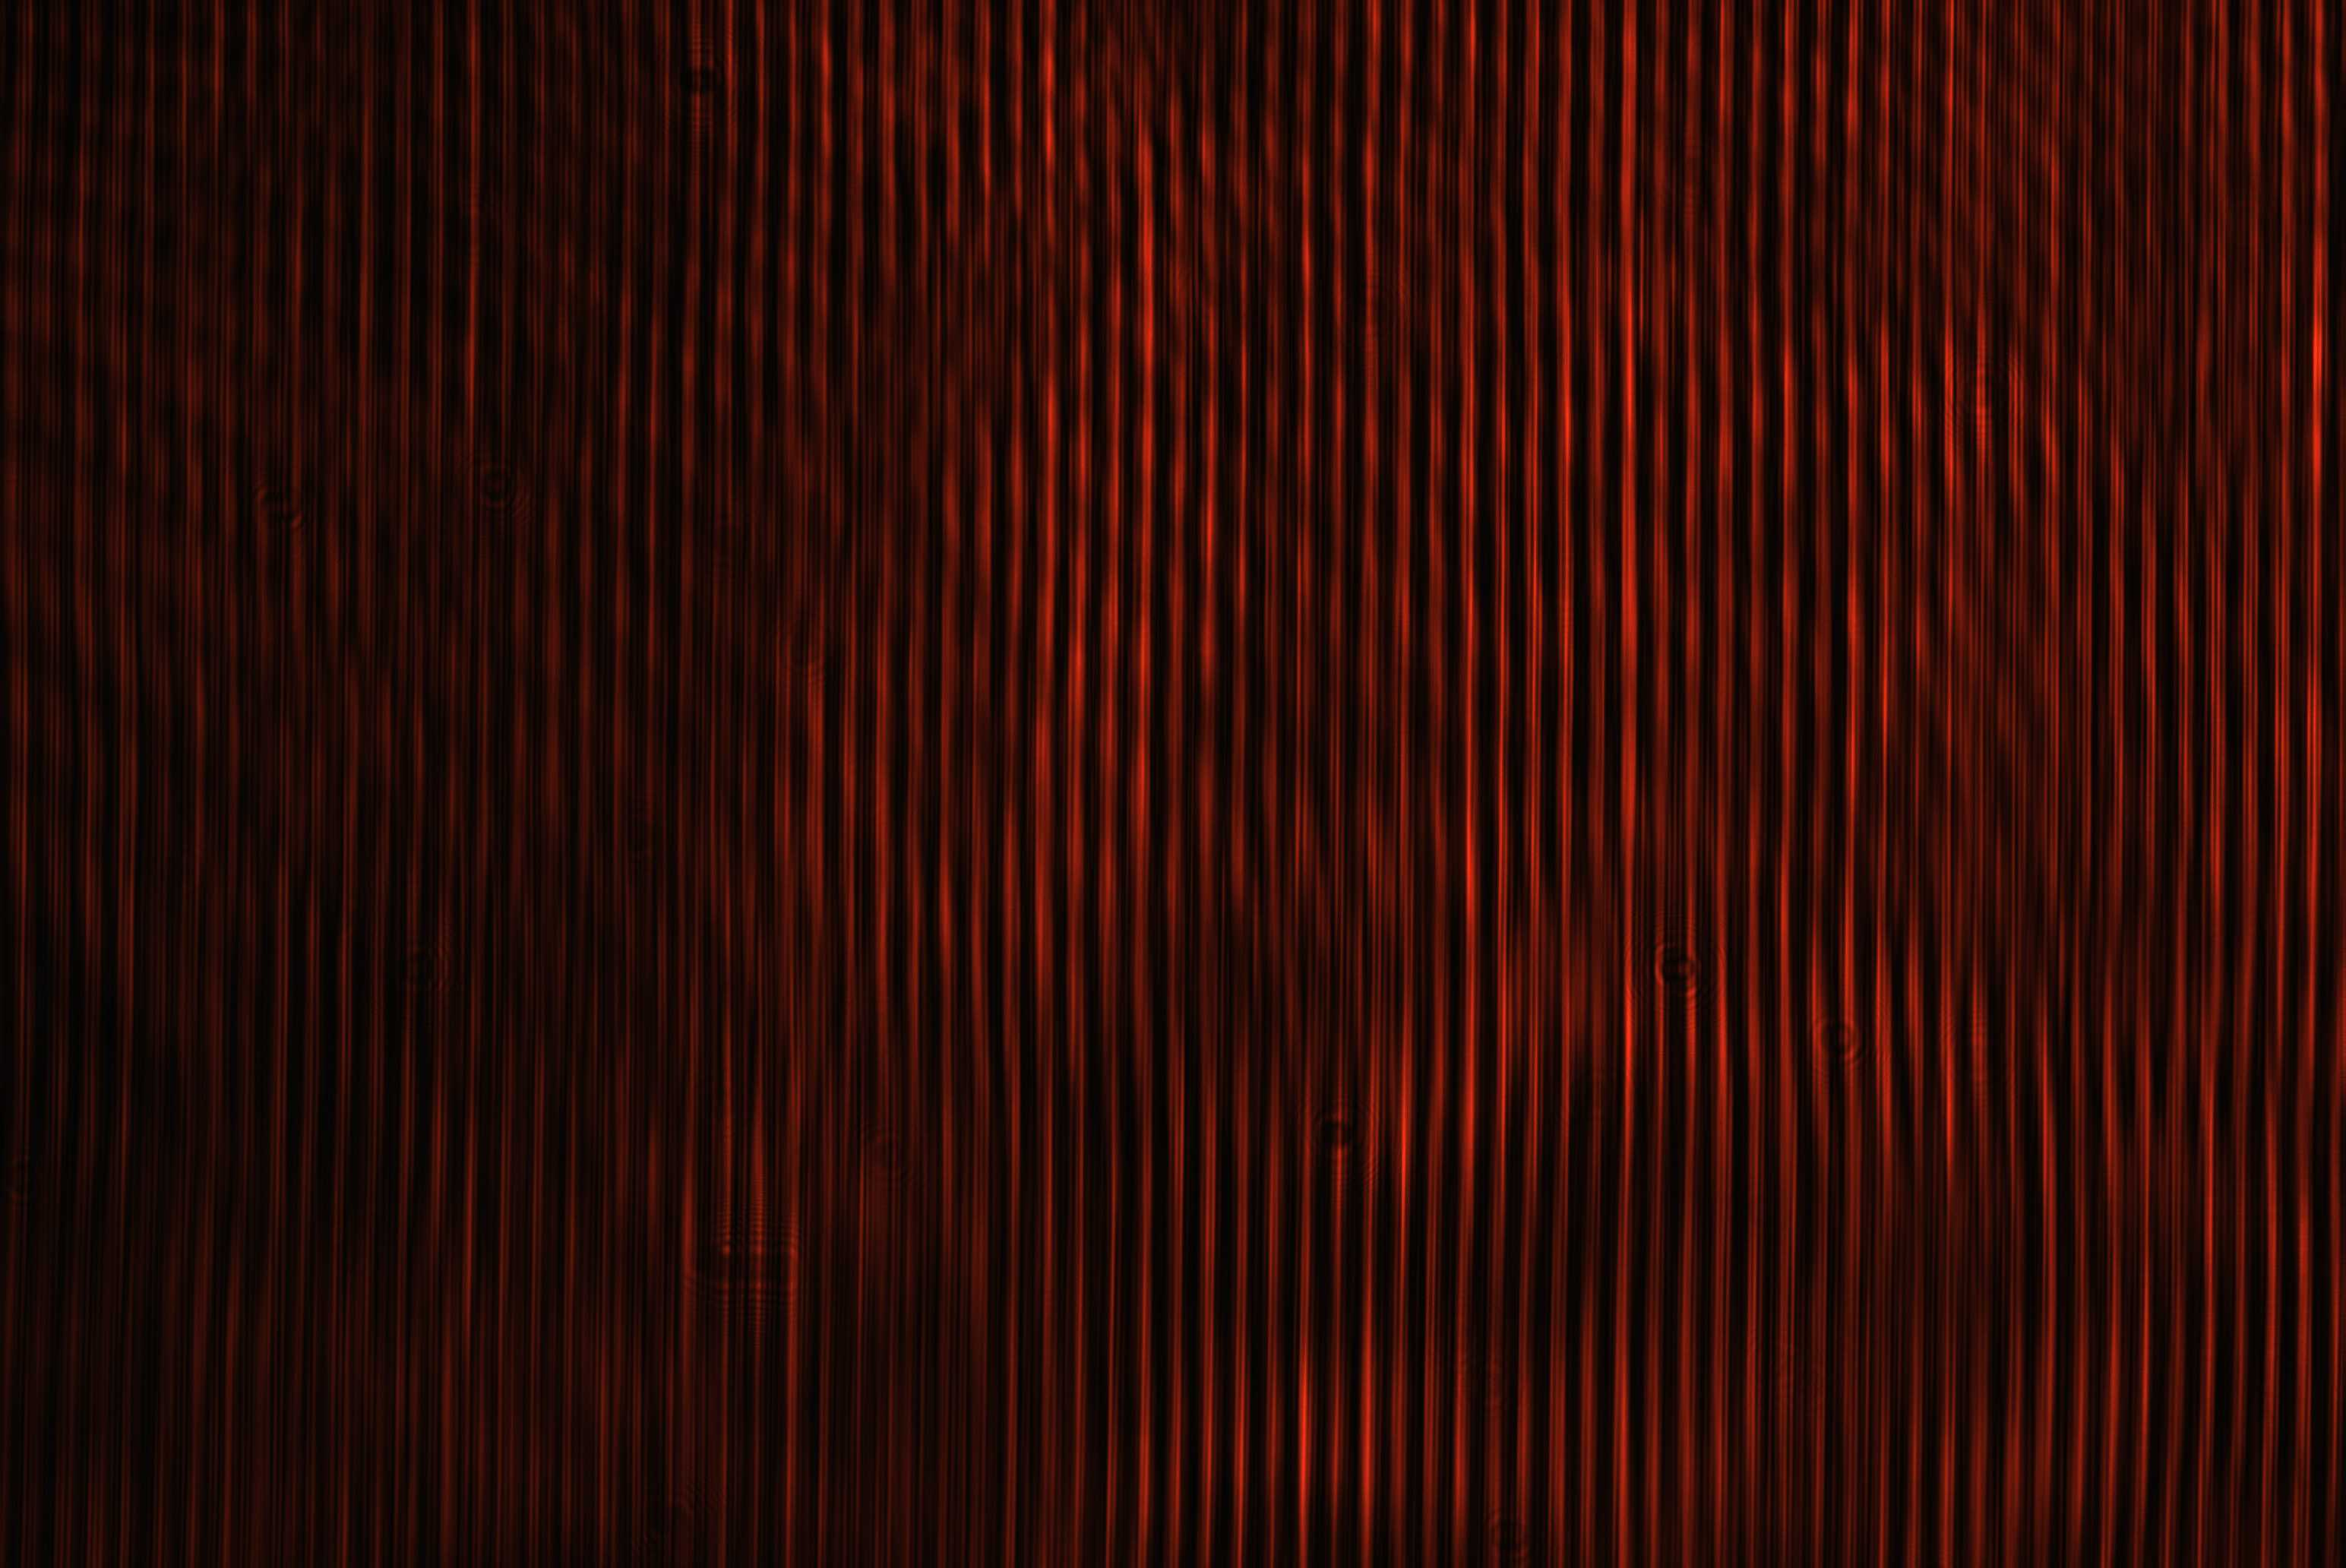
\includegraphics[width=0.24\textwidth]{attachments/fig.3.3.2.6.jpg}
			}
			\caption{\textbf{Band-pass filtering in different orientations }}
			\label{fig.3.3.2}
		\end{figure*}
		
		\begin{table*}[htbp]
			\centering
			\caption{\textbf{Band-pass filtering in different orientations}}
			\label{tab.3.1}
				\begin{tabular}{lllll}
					\toprule
					Orientation &$0^{o}$ & $45^{o}$ &$90^{o}$ & $135^{o}$ \\
					\midrule
					Pixels per 10 fringes & 446 & 325 &489 & 338 \\
					\bottomrule
				\end{tabular}
		\end{table*}

	\subsection{Holography}
		\subsubsection{Computational holography}
		Fig. \ref{fig.4.1} and Fig. \ref{fig.4.2} show the results of computational holography. 
		Computational holograms were initially generated from the original images using the Fourier transformation method.
		Then we loaded the holograms into the SLM and used the reference light to reconstruct the images.
		We found that both holograms were reconstructed correctly, which shows the effectiveness of computational holography.

		One classical computational holographic algorithm, named GS algorithm, is provided in Supplementary Information.

		\begin{figure*}[htbp]
			\centering
			\subfloat[Computational hologram]{
			
\includegraphics[width=0.4\textwidth]{attachments/fig.4.1.1.jpg}
			}
			\subfloat[Reconstructed image]{
			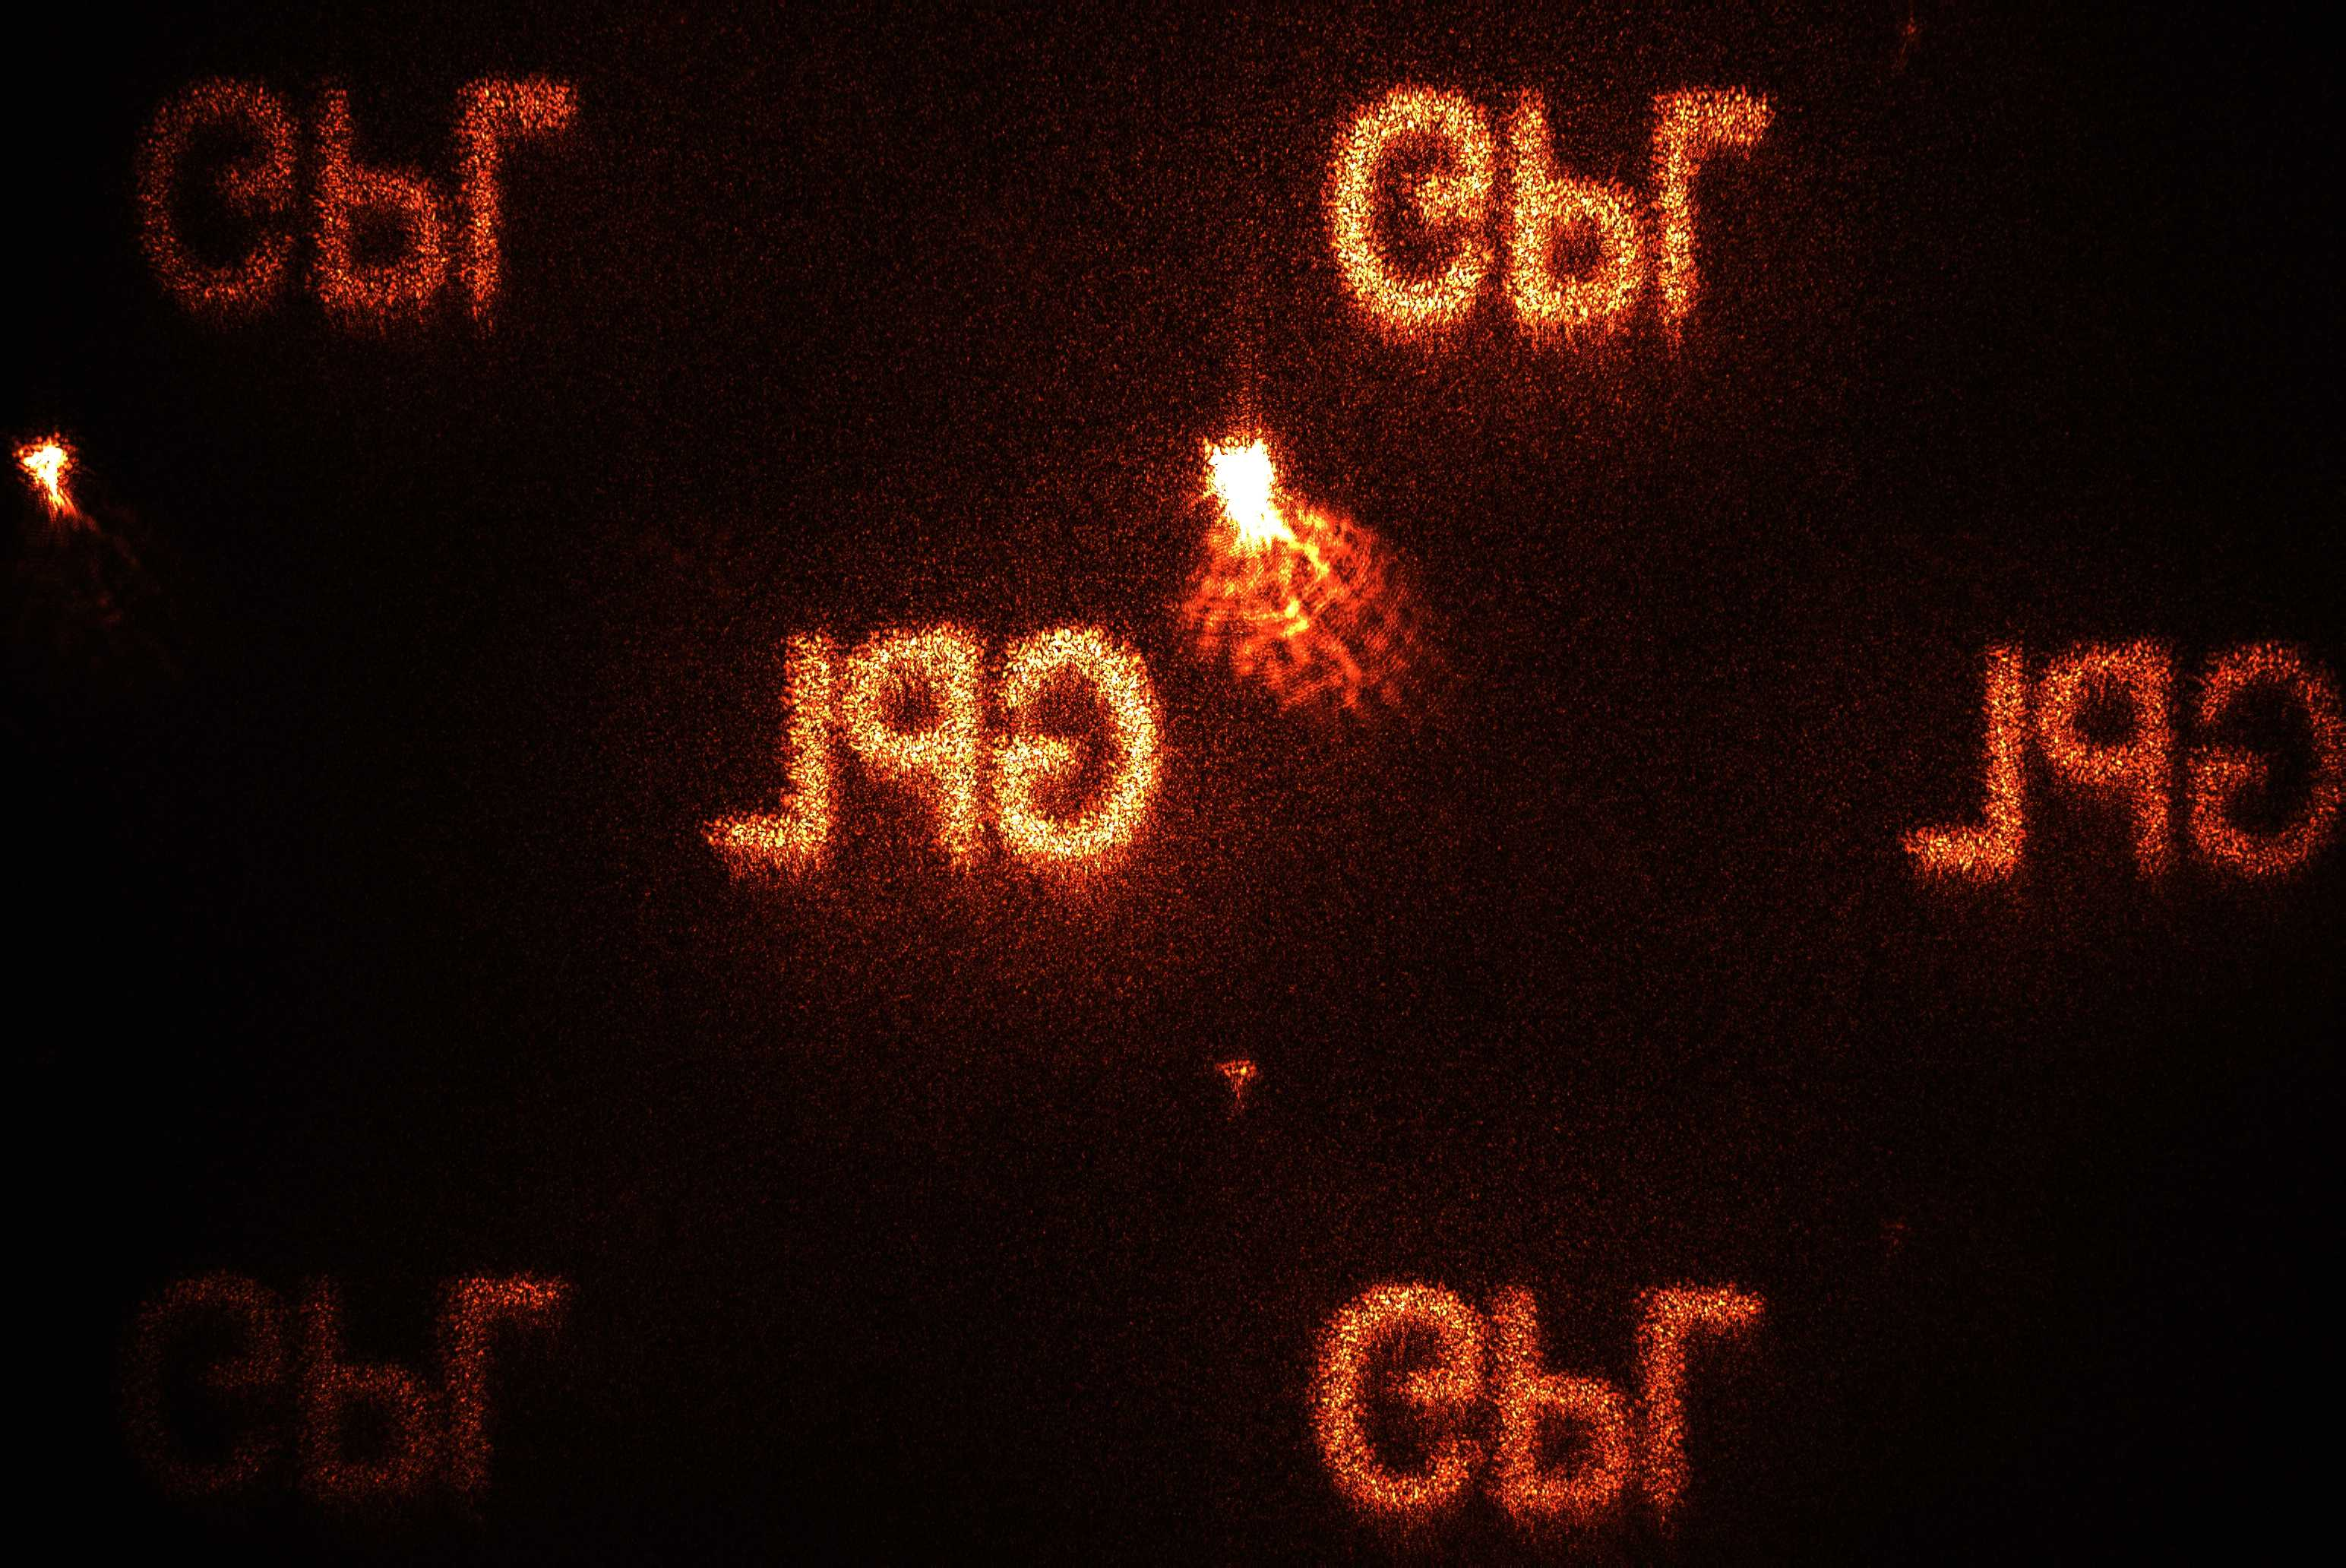
\includegraphics[width=0.4\textwidth]{attachments/fig.4.1.2.jpg}
			}
			\caption{\textbf{Computational holography: GPL image}}
			\label{fig.4.1}
		\end{figure*}

		\begin{figure*}[htbp]
			\centering
			\subfloat[Original image]{
			
\includegraphics[width=0.25\textwidth]{attachments/fig.4.2.1.jpg}
			}
			\subfloat[Computational hologram]{
			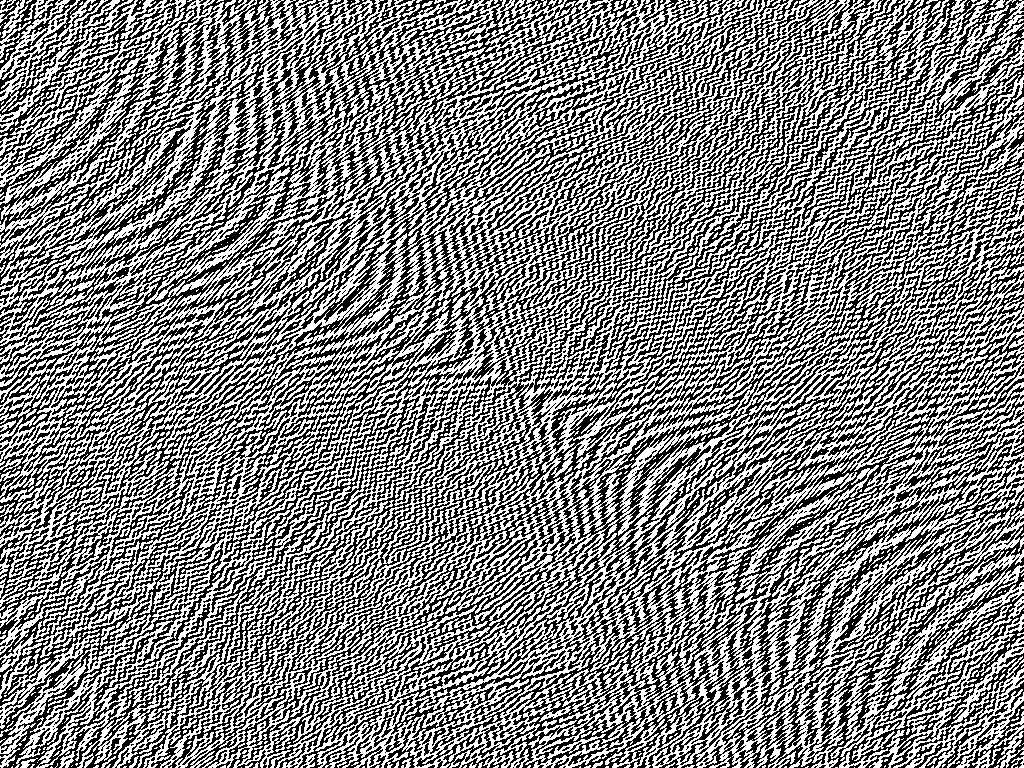
\includegraphics[width=0.25\textwidth]{attachments/fig.4.2.2.jpg}
			}
			\subfloat[Simulated Reconstructed image]{
			
\includegraphics[width=0.25\textwidth]{attachments/fig.4.2.3.jpg}
			}
			\subfloat[Reconstructed image]{
			\includegraphics[width=0.25\textwidth]{attachments/fig.4.2.4.jpg}
			}
			\caption{\textbf{Computational holography: SYSU image}}
			\label{fig.4.2}
		\end{figure*}

		\subsubsection{Digital holography}
		The reconstruction light path is illustrated in Fig. \ref{fig.illus-5.4}. 
		The hologram generated by adding a reference light onto the original object light field was recorded and reconstructed by the software.
		The results show that the image is correctly reconstructed. For comparison, the interference light field without the object was also recorded and reconstructed.
		An example algorithm is provided in Supplementary Information.

		\begin{figure*}[htbp]
			\centering
			\subfloat[Hologram]{
			\includegraphics[width=0.25\textwidth]{attachments/fig.4.3.1.jpg}
			}
			\subfloat[Reconstructed image]{
			\includegraphics[width=0.25\textwidth]{attachments/fig.4.3.2.jpg}
			}
			\subfloat[Reference hologram]{
			\includegraphics[width=0.25\textwidth]{attachments/fig.4.3.3.jpg}
			}
			\subfloat[Reference reconstructed image]{
			\includegraphics[width=0.25\textwidth]{attachments/fig.4.3.4.jpg}
			}
			\caption{\textbf{Digital holography}}
			\label{fig.4.3}
		\end{figure*}

%%end-------------------Result-----------------------%%

% %%begin-------------------Conclusion and Discussion-----------------------%%
\section{Conclusion and Discussion}
	\subsection{Conclusion}
	In this research, we investigated the properties of the spatial light modulator (SLM) and conducted a series of SLM-based optical experiments
	including detecting the distortion of the convex lens imaging system, optical information processing and holography.
	These results prove the high performance and effectiveness of SLM in optical experiments as a replacement for conventional optical elements.
	Our research may provide a new perspective for the application of SLM in optical experiments.

	\subsection{Known limitation}
		\begin{enumerate}[label=\arabic*.]
			\item In the experiment of measuring the distortion of the convex lens imaging system, actual image heights were measured manually, which might lead to great uncertainty. 
				  We have tried to use $OpenCV$ to automatically detect the edges of the check and measure height, but the performance of our codes was not satisfied.
				  The codes are accessible in our Github repository. Any improvements are welcomed and appreciated.
			\item Due to the relatively weak light power, the brightness of the image after low-pass filtering was too low to be seen clearly. Increase the light power may address this limitation.
			\item Although all images were correctly reconstructed in the holography experiment, the quality were still not quite satisfied. 
				  Precise adjustment of the light path and parameters may be required to further improve the performance.
		\end{enumerate}


%%end-------------------Conclusion and Discussion-----------------------%%

%%begin--------------------Reference------------------------%%
\printbibliography[title=Reference] 
%%end--------------------Reference------------------------%%
\end{document}